% !TEX program = xelatex
% 2026 高教社杯全国大学生数学建模竞赛 C 题：微网与外部电网电力调控策略
%
% 主控文件：只保留文档类、论文元数据与模块装配，正文内容不写入本文件。
%
% 目录结构
%   preamble/   导言区模块
%                packages.tex  本文额外需要的宏包
%                fonts.tex     编码、中文字体与字符类
%                layout.tex    版式、图形路径与全局排版参数
%   sections/   正文，文件名前缀与 \section 顺序一一对应
%                00-abstract        摘要页
%                01-restatement     一、问题重述
%                02-analysis        二、问题分析
%                03-assumptions     三、模型假设与符号说明
%                04-problem1        四、问题一：确定性日调度模型
%                05-problem2-model  五、问题二：序贯决策模型
%                06-problem2-results 六、问题二的结果分析
%                07-problem3        七、问题三：滚动合同调整模型
%                08-problem4        八、问题四（留白待补）
%                09-evaluation      九、模型评价
%   backmatter/ 参考文献与附录
%   figures/    正文配图（矢量 PDF，由 \graphicspath 统一解析）
%   code/       附录程序清单（fancyvrb 逐字输入）
%
% 标签命名规范：sec:qN-name / fig:qN-name / tab:qN-name / eq:qN-name / app:name，
% 正文一律用 \ref / \eqref / \S\ref 交叉引用，不写死编号。
%
% 配图取自 问题一/图片、问题二/图片 与 问题三/图片（矢量 PDF）；
% 附录核心程序摘自 问题一/算法 与 问题二/代码。
%
% 编译：latexmk -xelatex main.tex
% 说明：参考文献为 thebibliography 手工条目，全程不调用 bibtex / biber。
% =========================================================================

\documentclass[UTF8,a4paper,zihao=-4,fontset=windows]{ctexart}

% =========================================================================
% 宏包声明
% -------------------------------------------------------------------------
% 第一行是本模板的样式文件，随后是本文额外的宏包。
% cumcm2026.sty 已统一加载以下宏包，本文不再重复声明：
%   geometry, amsmath, amssymb, amsthm, mathtools, graphicx,
%   booktabs, tabularx, multirow, float, caption, enumitem,
%   xcolor, listings, fancyhdr, hyperref
%
% 注：本机 minted 不可用（需 -shell-escape 与 Pygments），故附录程序清单
%     统一使用 fancyvrb 的 \VerbatimInput 逐字输入，不使用 minted 环境。
% =========================================================================

% 模板样式：版式、页码、摘要环境、\mcmkeywords 与超链接设置均在此。
\usepackage{cumcm2026}

% 附录程序清单的逐字输入命令 \VerbatimInput。
\usepackage{fancyvrb}

% =========================================================================
% 编码与中文字体配置
% -------------------------------------------------------------------------
% 编码：由 \documentclass[UTF8]{ctexart} 一次性声明，源文件统一为 UTF-8（无 BOM）。
% 字体：由 \documentclass 的 fontset=windows 一次性指定，即
%       SimSun（正文）/ SimHei（标题）/ FangSong / KaiTi，
%       避免在其它平台静默换用别的中文字体而改变版面与分页。
%       中文换行、标点处理与 xeCJK 均由 ctex 宏包自动加载，无需重复声明。
% =========================================================================

% 带圈数字 ①~⑳ 与希腊字母默认被判为西文字符，而西文主字体不含这些字形，
% 会渲染成空白。显式划入 CJK 字符类，交由中文字体渲染。
% 范围：U+2460--U+2473 带圈数字；U+0370--U+03FF 希腊字母。
\xeCJKDeclareCharClass{CJK}{"2460 -> "2473, "0370 -> "03FF}

% =========================================================================
% 版式、图形路径与全局排版参数
% -------------------------------------------------------------------------
% 页面尺寸、页边距、页码位置、各级标题字号、行距、浮动体标题样式与
% 超链接颜色均由 cumcm2026.sty 统一设定，本节只补充本文档需要的项。
% =========================================================================

% 图形统一从 figures/ 解析，正文中只写文件名，不再重复目录前缀。
\graphicspath{{figures/}}

% 中文长行难免出现难以断行的段落，给 TeX 额外的伸缩余量，
% 避免产生 Overfull \hbox（默认 0pt）。
\emergencystretch=2em


\title{微网与外部电网电力调控的储能调度与购电策略优化}
\mcmkeywords{储能调度；线性规划；分位数预测；星期偏差校正；序贯决策；滚动合同调整；双向违约电价}

\begin{document}

% =========================================================================
% 摘要页（front matter）
% =========================================================================

\pagenumbering{arabic}
\begin{mcmabstract}
  本文研究微网与外部电网电力调控中的储能调度与购电策略。四问共用同一储能物理模型（容量 12000 kWh、允许储电量 $[1200,10800]$ kWh、充放电功率上限 5000 kW、双向效率 90\%），差别在于决策时可用的信息与结算规则：问题一为给定输入下的确定性日调度；问题二引入未来负载与光伏的未知性，缺口按 5 倍电价惩罚；问题三在问题二之上增加 6:00、12:00、18:00 三个预报时刻，并允许付费重定合同；问题四把电价本身变为逐区间波动的实时价。全文以``统一物理层＋各问新增信息与决策权限＋受控对照''为主线，目标为最小化购电费用。

  针对\textbf{问题一}，将一天离散为 144 个 10 分钟区间，建立以全天购电费用最小为目标的线性规划，并证明充放电互斥约束的线性松弛在最优值意义下精确，从而无需引入整数变量。以 HiGHS 求得的策略为：全天购电费 \textbf{35126.95 元}、购电量 59482.70 kWh，较无储能基准（48052.05 元）\textbf{节省 26.90\%}。

  针对\textbf{问题二}，构造``预测—计划—执行''三层滚动框架：预测层以近期净负载水平、星期偏差校正与分位裕量三项叠加给出当日预测；计划层求解带日循环边界的日前线性规划；执行层按净缺口符号即时尽限充放电，不足部分按 5 倍电价紧急购电。预测器形式、窗口长度与裕量水平均按逐月 walk-forward 协议选取，严格排除数据泄漏。评价期（2025.2.1--12.31，共 334 天）总费用 \textbf{1395.70 万元}，其中紧急费用占 5.5\%。

  针对\textbf{问题三}，在问题二框架上增设\textbf{调整层}：0:00 用附件 3 预报经分档收缩回归修正净负载预测，6:00、12:00、18:00 在实测储电量下对剩余时段重解带双向违约价（下调 $0.5p$、上调超出部分 $1.5p$）的线性规划，并证明该含分段的结算规则可由\emph{单个}线性规划精确表示。以``是否使用 0:00 预报通道 $\times$ 是否允许日内调整''构造 $2\times2$ 对照，主方案总费用 \textbf{1345.71 万元}，较问题二降费 \textbf{49.99 万元}，两项改进存在 9.62 万元的重叠。对题面所问``是否需要引入其他时刻的预报''，在本文所比较的全融合与逐点门控两种策略下，日内新增预报均未进一步降低费用（分别增费 9.59 与 6.08 万元）——双向违约价削弱了预测精度向费用节省的转化渠道。

  针对\textbf{问题四}，在附件 4 的逐区间实时价下重算问题二与问题三两条链路。价格的结构分析表明，实时电价接近``分时形状固定、日水平浮动再叠加小残差''的形式；据此可得\textbf{价格缩放不变性}，即价格的整体水平不产生决策价值，决策只依赖其归一化形状。模型层面引入两项修改：按价格形状加权的\textbf{价格加权风险裕量}，以及把优化终点延至次日 24:00 的 \textbf{48 小时滚动时域}（次日仅用持久性预测，信息严格因果）。两条分支的主方案费用分别为 \textbf{1438.23 万元}与 \textbf{1404.24 万元}；48 小时时域使两分支分别降费 \textbf{11.08 万元}与 \textbf{6.70 万元}，并在共同终端条件下保持。三个不含未来信息的在线选择器均未超过同年探索性选定的固定参数。
\end{mcmabstract}

\clearpage


% =========================================================================
% 一、问题重述
% =========================================================================

\section{问题重述}

\subsection{问题背景}

微网是为解决光伏发电等分布式能源本地消纳而发展起来的小型发用电系统。出于经济性考虑，非孤岛式微网可在外部电网（外网）电价较低或分布式能源有剩余电量时为储能设备充电，在电价较高时释放电能。储能设备最大容量 12000 kWh，允许储电量范围 1200--10800 kWh，最大充放电功率 5000 kW，充放电效率均为 90\%；2025 年 1 月 1 日 0:00 储电量为 6000 kWh。微网供电不得低于小区负载，富余供能可弃置，不向外部电网售电。附件 1 给出代表日 10 分钟间隔的电价、小区负载与光伏发电预测功率；附件 2 给出 2025 年逐日实测负载与光伏功率。

\subsection{四问对比}

题面四问共享同一物理系统，差别只在决策时可用的信息与可调整的决策。表~\ref{tab:restate} 按``可用信息—可调决策—新增难点''三条线把四问压缩对照：可用信息决定决策时能看多远，可调决策刻画各问授予的自由度，新增难点则是相对前一问必须额外处理的部分。

\begin{table}[H]
  \centering
  \caption{四问的信息条件、决策自由度与核心新增难点}
  \label{tab:restate}
  \small
  \begin{tabularx}{\textwidth}{@{}l >{\raggedright\arraybackslash}X >{\raggedright\arraybackslash}X >{\raggedright\arraybackslash}X@{}}
    \toprule
    问题 & 决策时可用信息 & 可调整的决策 & 核心新增难点 \\
    \midrule
    Q1 & 给定代表日电价、负载及光伏输入 & 0:00 购电计划、确定性储能轨迹 & 损耗与峰谷价差 \\
    \addlinespace
    Q2 & 已发生历史与已知分时电价；当日未来实测不可用（本文信息假设） & 日前计划锁定，执行按当前净负载反馈 & 预测偏差与 5 倍紧急费 \\
    \addlinespace
    Q3 & 增加附件 3 多次发布的光伏预报 & 6/12/18 时可改未来合同 & 信息价值、调整成本、实际 SOC \\
    \addlinespace
    Q4 & 增加实时波动价格；未来价格不可见（本文解释） & 分别继承 Q2/Q3 权限 & 相对价格与跨日库存配置 \\
    \bottomrule
  \end{tabularx}
\end{table}

\subsection{必答交付物}

四问均要求给出可复算的具体结果。问题一至问题三按题目表 1 格式给出指定时间段的购电量、全天购电量与购电费，按表 2 格式给出指定时间段的充放电量与 0:00、24:00 储电量；问题二、问题三另按表 3 格式给出紧急购电结果。其中问题一针对代表日，\textbf{问题二、问题三还需分别给出 2025 年 3 月 20 日、6 月 21 日、9 月 23 日、12 月 21 日四个指定日期的表 1、表 2 与表 3 结果}。问题四在实时电价下分别按``仅 0:00 计划''与``0:00 计划＋三次调整''两种决策结构重算，并按同样的表式给出结果。全部策略依次保存到 \texttt{result1.xlsx}--\texttt{result4-3.xlsx}。

% =========================================================================
% 二、问题分析
% =========================================================================

\section{问题分析}

四问共享同一物理系统与同一储能约束，差别在于\textbf{信息条件与结算规则}。因此本文的问题分析统一采用``新约束或信息变化 $\to$ 为什么原方法不足 $\to$ 本文作何修改''的三步框架，把定量结果与对照留到各问的结果分析，不在前置分析中提前宣布结论。技术路线随之从单日线性规划升级为``预测—计划—执行''三层滚动框架（\S\ref{sec:q2-frame}），再扩展为``计划—调整—执行''三层结构（\S\ref{sec:q3-frame}），最后在价格侧引入不确定性并延展优化时域（\S\ref{sec:q4-model}）。

\subsection{问题一：时段转移与富余吸收}

\textbf{信息与约束变化。}当天负载与光伏均视为已知，决策退化为确定性优化；但储能把各区间耦合起来——当前区间的充放电通过储电量影响后续所有区间。

\textbf{原方法的不足。}逐区间贪心无法处理上述跨时段耦合；而物理上储能不可同时充放电（$c_td_t=0$），直接引入该约束将使模型非线性，失去求全局最优的条件。

\textbf{本文的修改。}建立全天联合的线性规划（\S\ref{sec:q1-constraint}）；并在 \S\ref{sec:q1-relax} 证明互斥约束的线性松弛在最优值意义下精确，模型保持为可求全局最优的线性规划。

\begin{figure}[H]
  \centering
  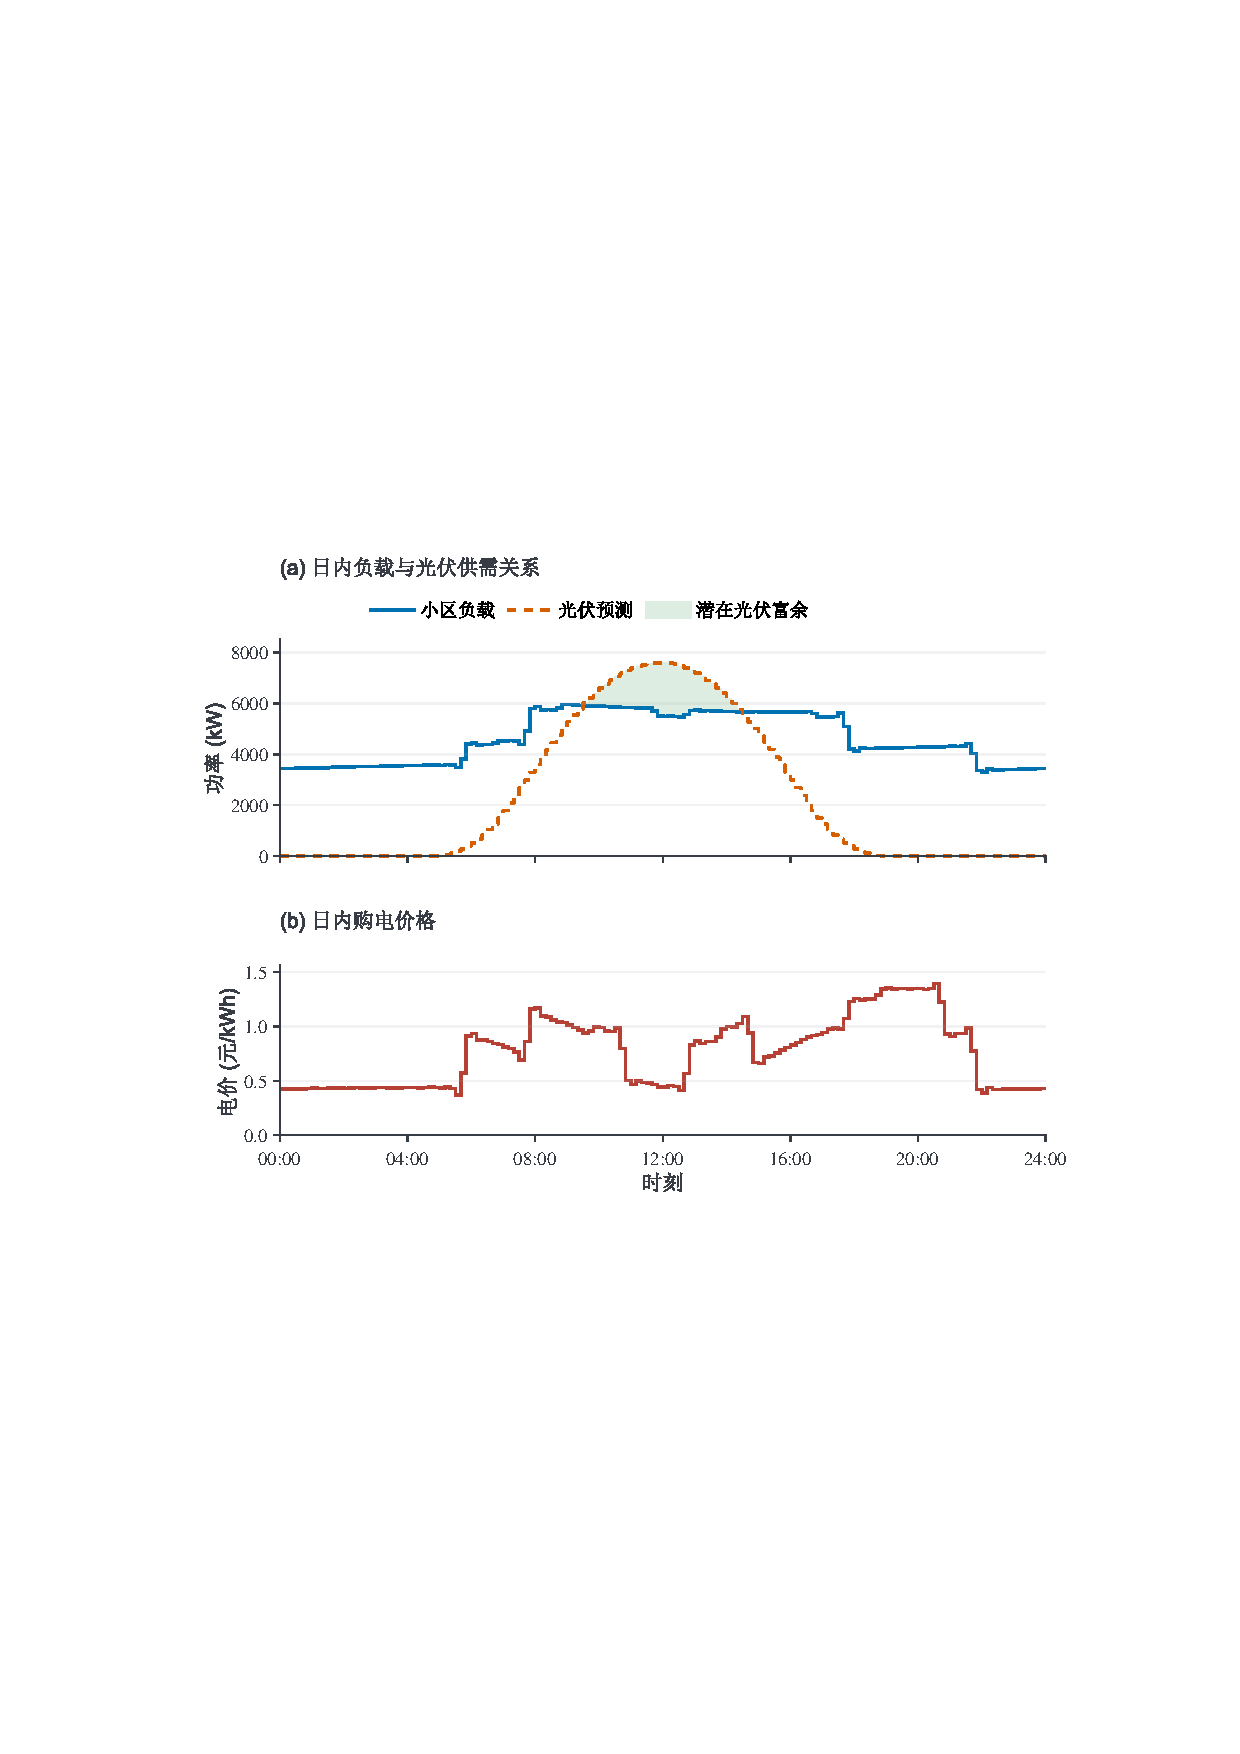
\includegraphics[width=0.82\textwidth]{p1_fig1.pdf}
  \caption{代表日输入特征：小区负载、光伏预测功率与电价曲线}
  \label{fig:q1-input}
\end{figure}

\subsection{问题二：不对称代价下的序贯决策}

\textbf{信息与约束变化。}计划只能基于预测，实测偏差必须按 5 倍电价紧急补足。这一惩罚使代价结构高度不对称：少计划 1 kWh 的期望代价远高于多计划 1 kWh 的代价。

\textbf{原方法的不足。}逐日实测净负载同时含有星期周期与随季节缓慢漂移的近期水平两层可预测结构。只用近期水平会平滑掉星期形状，只用代表日曲线又跟不上季节漂移；此外，任何用``当天实测''改善``当天计划''的做法都不可实施，需要用一条明确的信息纪律把这种泄漏排除掉。

\textbf{本文的修改。}预测层显式分解为``近期水平＋星期偏差''两层，再叠加用于吸收残余随机性的分位裕量（\S\ref{sec:q2-forecast}）；计划层保持线性规划（\S\ref{sec:q2-lp}）；执行层采用完全因果的尽限充放电规则，在净缺口出现时即时释放可用电量（\S\ref{sec:q2-exec}）；参数按逐月 walk-forward 协议选取（\S\ref{sec:q2-walkforward}）。

\subsection{问题三：信息增加与调整机会的价值辨析}
\label{sec:q3-analysis}

\textbf{信息与约束变化。}题面并未要求``利用更多预报提高预测精度''，而是要求分析\textbf{是否需要}引入其他时刻的预报。除新增 6:00、12:00、18:00 三个预报时刻外，还允许对这些时刻之后的购电量\textbf{重新约定}，代价是相对 0:00 计划的偏离要按双向违约价付费。

\textbf{原方法的不足。}问题二的一次性决策无法利用日内信息，这是明确的改进方向；但``信息更多''与``费用更低''之间不存在必然的对应关系，需要分别计量两条作用渠道：其一，调整机会本身有价值——白天若发现净负载低于预期，可下调合同并按违约价结算；其二，调整本身有摩擦——双向违约价使``偏离 0:00 计划''成为独立成本项，且该成本与预测精度直接耦合，预测越激进地偏离基准，重定合同的动作越大。此外，两项改进可能部分替代：已有第二次决策机会时，0:00 预报的边际价值会被削弱。

\textbf{本文的修改。}插入\textbf{调整层}，形成``计划—调整—执行''三层结构（\S\ref{sec:q3-frame}、\S\ref{sec:q3-adjust}）；并采用 $2\times2$ 对照（\S\ref{sec:q3-matrix}）而非简单相减来计量``信息''与``调整机会''各自的收益及其重叠。

\subsection{问题四：价格侧不确定性的来源辨析与信息边界}
\label{sec:q4-analysis}

\textbf{信息与约束变化。}问题二、问题三的不确定性全部位于负载与光伏一侧，问题四新增了价格一侧：电价由已知量变为逐区间的随机量，且按本文解释随区间推进逐步揭示。

\textbf{原方法的不足。}两处需要修改：其一，问题二的均一分位裕量对所有时段取同一分位水平，未反映``缺口发生在高价时段时单位代价更高''这一事实；其二，日循环边界限制的是\textbf{计划中的单日净库存变化}，在固定电价下这一限制尚不显著，而在实时价格下，低价夜间若不能把电量安排在更晚的时段使用，低价优势无法充分利用。同时，两张不确定性谁更重要不能凭直觉判断，需要先分解价格的统计结构，再分别标定两侧信息的经济价值。

\textbf{本文的修改。}先作价格结构分解与价格缩放不变性分析（\S\ref{sec:q4-struct}、\S\ref{sec:q4-scaling}），据此把价格预测的目标由``全曲线''压缩到``归一化形状''；模型层面引入按价格形状加权的风险裕量（式~\eqref{eq:q4-prm}），并把优化时域延展到次日 24:00（\S\ref{sec:q4-horizon}），同时在信息侧严格保持因果（次日只用持久性预测）；结果以同政策对照、终端条件一致性与放松下界参照分别检验（\S\ref{sec:q4-ablation}、\S\ref{sec:q4-regret}）。

% =========================================================================
% 三、模型假设与符号说明
% =========================================================================

\section{模型假设与符号说明}

以下把假设按\textbf{题面给定}、\textbf{解释与近似}、\textbf{算法与评价设计}三类分列。区分的意义是：第一类是题目条件，不作为本文的自设假设；第二类是可被质疑的口径，逐条给出依据与影响；第三类是实现方案的选择，不是客观事实，其取值在正文相应位置说明。

\subsection{题面给定的参数与条件}

\begin{enumerate}
  \item 储能最大容量 12000 kWh，允许储电量范围 $[1200,10800]$ kWh，最大充放电功率 5000 kW，充放电效率两向各 90\%（附录 1）；
  \item 允许供能余量（富余供能可弃置），微网不向外部电网售电、不产生售电收入；
  \item 问题一要求储能设备在 0:00 与 24:00 的储电量相同；
  \item 问题二、问题三、问题四中，供电低于负载时须按交易时刻电价的 5 倍\textbf{紧急购电}；
  \item 问题三、问题四的 Q3 分支中，计划购电量高于调整购电量的部分按交易时刻电价的 50\% 结算，调整购电量高于计划购电量的部分、其超出部分按交易时刻电价的 1.5 倍结算；
  \item 问题四的电价为附件 4 给出的逐 10 分钟区间实时电价，计划购电与调整购电均按该区间实时价结算。
\end{enumerate}

\subsection{解释与近似}

以下五条不是题面给定的事实，而是本文对题面未明示之处的读法。逐条给出依据与影响。

\begin{enumerate}
  \item \textbf{问题二的信息口径}：第 $d$ 天 0:00 决策时只可用第 $1,\dots,d-1$ 天的实测与附件 1 的曲线，当日及以后的实测值及其派生量一律不可用；决策规则超参数的选取同样受此约束。依据：题面要求``每天 0:00 制定当天计划''，计划不可能包含当日实测。影响：这是问题二与问题三全部预测逻辑的前提。
  \item \textbf{问题四的价格揭示口径}：附件 4 给出的是各区间\emph{已发生}的实时电价，故价格随区间推进逐步揭示——0:00 只知前一日及以前的价格，6:00、12:00、18:00 另知当日已过去区间的价格，任何决策均不使用尚未揭示区间的电价。影响：该口径的替代方案（日前已知全天价）在同一政策下相差 7.70 万元，其量化见 \S\ref{sec:q4-sens}。
  \item \textbf{功率数据按区间平均功率读}：附件 1、附件 2 的时间标记为区间末端，但题面未给出功率数据的定义。本文统一把附件值读作该 10 分钟\emph{区间}的平均功率，并以区间电量 $=P\,\Delta t$ 折算。影响：若实际定义为瞬时值，量纲折算需改为数值积分，本文的逐区间口径随之改变。
  \item \textbf{附件 3 预报的时间约定}：$f_\tau(h)$ 定义为\textbf{发布后第 $h$ 小时}的整点光伏功率预报，区间电量按相邻整点线性插值后在区间上积分得到（式~\eqref{eq:q3-pv}）。发布时刻 $\tau>0$ 时，首端点的功率取``上一已结束区间的平均功率''（由该区间电量除以 $\Delta t$ 换回 kW），这是对发布时刻瞬时功率的\textbf{端点近似}，不是直接观测到的瞬时值。影响：图~\ref{fig:q3-pv} 的对照表明该近似优于改用历史预报端点。
  \item \textbf{未建模的因素}：不引入题目未要求的电池退化成本、运维成本，不建模售电，也不把预测残差的时段间相关性显式写入规划模型。影响：这些因素会使实际的可行域与费用账本发生变化，故本文的全部结论限于上述口径。
\end{enumerate}

\subsection{算法与评价设计}

\begin{enumerate}
  \item \textbf{计划端的末端条件分问设定}：问题一的日循环是题面条件，直接写在模型约束中；问题二、问题三的计划层以``计划末端电量等于日初电量''作为单日规划的自洽边界，它\textbf{只约束计划轨迹，不约束实际运行}（实际日末电量可以不同于日初并结转到次日）；问题四的计划层把末端条件改为 48 小时时域末端回到起点（\S\ref{sec:q4-horizon}）。三者是不同问题的不同设计，不互相推广。
  \item \textbf{评价期与共同预热}：为消除各方案 1 月冷启动轨迹差异的干扰，所有可实施方案共用同一条 1 月预热轨迹，2 月 1 日 0:00 统一从 10800 kWh 起评，评价期为 2025.2.1--12.31 共 334 天；1 月仅用于提供历史数据与首次选参，不计入评价。
  \item \textbf{因果选参}：问题二的 $(\beta,W,\gamma,N_{\mathrm{DOW}})$ 按逐月 walk-forward 协议选取（\S\ref{sec:q2-walkforward}）；问题三的收缩系数 $\kappa_g$ 只用 $d$ 之前 30 天逐日重估。问题四的 $(\lambda_{\mathrm{p}},\delta)$ 与 48 小时时域为\textbf{同年探索性选定}——其逐时动作不读取未来信息，但候选范围的确定过程看过全年数据，两者不是一回事，本文在 \S\ref{sec:q4-selector}、\S\ref{sec:q4-limit} 如实标注，不宣称独立测试。
  \item \textbf{候选网格}：$W\in\{7,14\}$，$N_{\mathrm{DOW}}\in\{4,6,10\}$，$\gamma\in\{0,0.5,1.0\}$，$\beta\in\{0.70,0.75\}$（\S\ref{sec:q2-walkforward}）；问题四的 $\lambda_{\mathrm{p}}$、$\delta$ 按 \S\ref{sec:q4-grid} 的格点取定。网格边界处的最优性不作一般性断言。
  \item \textbf{分位裕量的独立性}：裕量按各时段单独取分位数，未建模时段之间的相关性；这将使同时段多区间同时缺口的联合概率不被显式控制。
\end{enumerate}

\subsection{时间离散口径}

附件 1/2 的时间标记为区间末端；区间 $t$ 指 $[t\Delta t,(t+1)\Delta t)$，$\Delta t = 1/6$ h，每日 $T=144$ 个区间。结合 \S 上文解释与近似中``功率数据按区间平均功率读''的口径，功率（kW）乘 $\Delta t$ 折算为电量（kWh）；电价为强度量，直接取附件值。问题一、二的结果文件均按官方模板原始行序填写，模板行标签较字面区间整体后移一个区间，核对时需注意。

\subsection{术语约定}

为保持全文用词一致，先作如下约定：

\begin{itemize}
  \item \textbf{预报}专指附件 3 给出的逐时光伏发电功率；\textbf{预测}专指本文模型给出的净负载估计；\textbf{点预测}指不含风险裕量的中心预测 $\mu$，\textbf{规划需求代理}指叠加裕量后进入规划的量 $\widetilde N$；
  \item \textbf{计划购电量}（记 $b^{0}$）指 0:00 制定的购电量；\textbf{最终合同购电量}（记 $b^{\mathrm f}$）指经调整层重定后实际执行与结算的购电量；\textbf{紧急购电量}指实测缺口超出储能释放能力后按 5 倍电价购入的电量；
  \item \textbf{供能余量}指已购或已发而未被消纳、最终弃置的电量；\textbf{光伏富余}指光伏出力高于同期负载的部分；
  \item \textbf{计划库存}（记 $\widehat E$）指线性规划轨迹上的储能电量；\textbf{实际库存}（记 $E$）指执行层按实测递推得到的储能电量；
  \item \textbf{实时电价}（仅见于问题四）指附件 4 给出的逐区间电价；\textbf{价格水平}指式~\eqref{eq:q4-decomp} 中的日水平因子 $\ell_d$；\textbf{价格形状}指归一化后的日内价格轮廓；
  \item \textbf{滚动时域}（问题四）指把计划线性规划的优化终点由当日 24:00 延至次日 24:00 的做法；\textbf{持久性预测}指以当日预测序列平铺来估计次日输入的近似方式；
  \item \textbf{方案}指一组可完整执行的配置（A、B、E、A0、A0K、B0、B1、F\_48、G\_48 等）；\textbf{策略}沿用题面含义，指逐日制定购电决策的规则。
\end{itemize}

\subsection{符号说明}

\begin{table}[htbp]
  \centering
  \caption{主要符号说明（问题一至问题三）}
  \label{tab:sym-common}
  \small
  \begin{tabularx}{0.9\textwidth}{cX}
    \toprule
    符号 & 含义 \\
    \midrule
    $t$ & 日内 10 分钟区间编号，$t=0,1,\dots,143$ \\
    $T=144$ & 每日区间数（固定）；$\Delta t=1/6$ h 为区间长度 \\
    $H$ & 单次优化问题的时域长度（区间数）：日计划 $H=T$，问题四的 48 小时计划 $H=2T$ \\
    $d$ & 日期编号，$d=0,\dots,364$（2025 年） \\
    $P^L_t,\ P^{PV}_t$ & 区间 $t$ 的负载、光伏平均功率（kW） \\
    $L_t,\ V_t$ & 区间 $t$ 的负载电量、光伏电量，$L_t=P^L_t\Delta t$，$V_t=P^{PV}_t\Delta t$（kWh） \\
    $N_t^{(d)}=L_t^{(d)}-V_t^{(d)}$ & 第 $d$ 天区间 $t$ 的\textbf{实测}净负载（kWh） \\
    $\mu_t$ & 净负载\textbf{点预测}（不含风险裕量，仅用历史信息） \\
    $\widetilde N_t$ & \textbf{规划需求代理}：点预测叠加风险裕量后进入线性规划的需求（kWh） \\
    $\widehat E_t,\ E_t$ & \textbf{计划}库存、\textbf{实际}库存（区间 $t$ 起始，kWh） \\
    $p_t$ & 区间 $t$ 的购电电价（元/kWh）；紧急电价为 $5p_t$ \\
    $b^{0}_t,\ b^{\mathrm f}_t$ & 0:00 计划购电量（日前合同）与最终合同购电量（kWh）；问题二无调整层，$b^{\mathrm f}_t=b^{0}_t$，正文简记 $b_t$ \\
    $c_t,\ d_t$ & 区间 $t$ 储能充电量、放电量（交流侧，kWh）；$\bar C=\bar D=5000/6$ kWh \\
    $e_t,\ w_t$ & 区间 $t$ 的紧急购电量、弃置供能余量（kWh） \\
    $\eta_c,\ \eta_d$ & 充电、放电效率，均为 $0.9$ \\
    $W,\ N_{\mathrm{DOW}}$ & 近期水平窗口长度（天）、同星期偏差所取的历史同星期日个数（天） \\
    $\gamma,\ \beta$ & 星期偏差校正强度、分位数裕量水平 \\
    \bottomrule
  \end{tabularx}
\end{table}

\begin{table}[htbp]
  \centering
  \caption{主要符号说明（问题三的预报通道与问题四的实时电价）}
  \label{tab:sym-q34}
  \small
  \begin{tabularx}{0.9\textwidth}{cX}
    \toprule
    符号 & 含义 \\
    \midrule
    $\tau$ & 预报发布时刻，$\tau\in\{0,6,12,18\}$（h）；对应区间 $t_\tau=6\tau$ \\
    $f_\tau(h)$ & 发布时刻 $\tau$ 对\textbf{发布后第 $h$ 小时}的整点光伏功率预报（kW）；$\widetilde V_t(\tau)$ 为其区间电量 \\
    $\kappa_g$ & 附件 3 预报通道的分档收缩系数，按预报时长分三档 \\
    $u_t,\ v_t$ & 合同相对 $b^{0}$ 的下调量、上调量（kWh），违约／加价分段 \\
    $\lambda$ & 门控实验中单决策点选用的预报融合强度，$\lambda\in\{0,\tfrac14,\tfrac12,1\}$ \\
    \midrule
    $P_{d,t}$ & 附件 4 给出的第 $d$ 天区间 $t$ 的实时电价（元/kWh）；结算时记 $p_t$ \\
    $\pi_t^{\mathrm{TOU}},\ \ell_d,\ r_{d,t}$ & 分时电价形状、日价格水平因子、价格残差（式~\eqref{eq:q4-decomp}） \\
    $\omega_t$ & 价格加权风险裕量的权重，由决策价形状按幂次生成，整日冻结 \\
    $\lambda_{\mathrm{p}},\ \delta$ & 价格加权强度（幂指数）与裕量水平偏移（式~\eqref{eq:q4-prm}） \\
    \bottomrule
  \end{tabularx}
\end{table}

% =========================================================================
% 四、问题一：确定性日调度模型
% =========================================================================

\section{问题一：确定性日调度模型的建立与求解}

\subsection{决策变量与目标函数}

将一天离散为 144 个 10 分钟区间。决策变量为各区间的计划购电量 $g_t$、储能充电量 $c_t$、放电量 $d_t$、供能余量 $w_t$（$t=0,\dots,143$）与各区间起始储电量 $E_t$（$t=0,\dots,144$），共 $4\times144+145=721$ 个变量，全篇统一采用电量口径。以全天计划购电费用最小为目标：
\begin{equation}
  \min\ J=\sum_{t=0}^{143}p_t\,g_t .
\end{equation}

\subsection{约束条件}
\label{sec:q1-constraint}

\begin{align}
  &g_t+V_t+d_t=L_t+c_t+w_t, \qquad E_{t+1}=E_t+\eta_c c_t-\frac{d_t}{\eta_d}, \label{eq:q1-balance}\\
  &1200\le E_t\le 10800, \qquad 0\le c_t,\ d_t\le \frac{5000}{6}, \label{eq:q1-bound}\\
  &g_t\ge 0,\quad w_t\ge 0,\qquad E_0=E_{144}=6000. \label{eq:q1-cycle}
\end{align}
式~\eqref{eq:q1-balance} 第一式为区间能量平衡（供＝需＋余量），第二式为储能递推（充电按 $\eta_c$ 存入、放电按 $\eta_d$ 折损）；式~\eqref{eq:q1-bound} 依次为储电量允许范围（附录 1）与充放电功率上限（5000 kW 折算为区间电量上限 $5000/6$ kWh）；式~\eqref{eq:q1-cycle} 为题目要求的日循环条件（日初日末储电量相等，取附录 1 给定的 6000 kWh）。

\subsection{充放电互斥约束的松弛精确性}
\label{sec:q1-relax}

物理上要求 $c_t d_t=0$。以下命题保证无需引入二元变量。

\begin{quote}
  \textbf{命题.} 在 \S\ref{sec:q1-constraint} 的模型中，存在一个满足充放电互斥的最优解，即线性松弛在最优值意义下精确。
\end{quote}

\textbf{证明.} 设某最优解在区间 $t$ 同时充放电，取 $\delta=\min(c_t,\ d_t/0.81)>0$，将该区间充电减少 $\delta$、放电减少 $0.81\delta$。则储能变化量不变：
\begin{equation}
  -0.9\delta+\frac{0.81\delta}{0.9}=0,
\end{equation}
$E_t,E_{t+1}$ 及全部储能约束不受影响；能量平衡式中供给减少 $0.81\delta$、用能减少 $\delta$，净余量增加 $0.19\delta\ge0$，由 $w_t$ 吸收，可行性保持；$g_t$ 与目标值不变。重复此操作即得满足互斥且目标不劣的可行解。$\blacksquare$

该约化不依赖电价非负；其条件为余量可自由增加、效率乘积 $\eta_c\eta_d\le1$，以及模型存在有限最优解。数值上，求得的最优解同时充放电重叠量为 0，与命题一致。

\subsection{求解流程与数值校验}

模型为 721 变量、290 个等式约束的线性规划，调用 SciPy 的 \texttt{linprog}（HiGHS 求解器~\cite{highs,scipy}）求解，返回最优解，共 367 次迭代。求解流程为：① 读取附件 1 并按区间末端口径折算电量；② 以稀疏矩阵装配线性规划；③ 由 HiGHS 求解；④ 独立校验——能量平衡与储能递推的最大残差 $<10^{-12}$ kWh，储电量全程位于 $[1200,10800]$，$E_0=E_{144}=6000$，充放电功率无越界，同时充放电重叠量为 0，购电费用独立复算与求解器输出一致（差 $<10^{-10}$ 元）；⑤ 按官方模板写出 \texttt{result1.xlsx}。全部结果可由 \texttt{scripts/q1\_solve.py} 一条命令复现，核心程序见附录~\ref{app:q1-code}。

\subsection{结果分析}

\subsubsection{最优购电与储能调度结果}

\begin{table}[H]
  \centering
  \caption{指定时间段的计划购电量及全天结果（对应题目表 1）}
  \label{tab:q1-t1}
  \begin{tabular}{cccc}
    \toprule
    时间段 & 购电量 (kWh) & 时间段 & 购电量 (kWh) \\
    \midrule
    10:00--10:10 & 0.0000 & 16:00--16:10 & 445.4317 \\
    12:00--12:10 & 480.4124 & 18:00--18:10 & 531.8940 \\
    14:00--14:10 & 0.0000 & 20:00--20:10 & 0.0000 \\
    \midrule
    \multicolumn{2}{l}{全天购电量} & \multicolumn{2}{l}{\textbf{59482.6990 kWh}} \\
    \multicolumn{2}{l}{全天购电费} & \multicolumn{2}{l}{\textbf{35126.9486 元}} \\
    \bottomrule
  \end{tabular}
\end{table}

\begin{table}[H]
  \centering
  \caption{储能设备在指定时间段的充放电量及 0:00、24:00 储电量（对应题目表 2）}
  \label{tab:q1-t2}
  \begin{tabular}{ccc}
    \toprule
    时间段 & 充电量 (kWh) & 放电量 (kWh) \\
    \midrule
    0:00--4:00   & 4500.0000  & 0.0000 \\
    4:00--8:00   & 833.3333   & 6365.8412 \\
    8:00--12:00  & 4787.9643  & 1702.9970 \\
    12:00--16:00 & 5286.0352  & 91.1014 \\
    16:00--20:00 & 0.0000     & 5780.1319 \\
    20:00--24:00 & 5333.3333  & 2859.8681 \\
    \midrule
    0:00 储电量 & \multicolumn{2}{c}{6000.0000 kWh} \\
    24:00 储电量 & \multicolumn{2}{c}{6000.0000 kWh} \\
    \bottomrule
  \end{tabular}
\end{table}

最优策略（图~\ref{fig:q1-strategy}）呈清晰的``三充两放''节律：\textbf{凌晨低价段}以功率上限充电，并在全日最低价区间（5:30，0.3713 元/kWh）再次满功率充电，5:40 储电量首次触及上限 10800 kWh；\textbf{早高峰（5:50--9:20）}放电替代约 0.69--1.17 元/kWh 的购电，储电量回落至约 1860 kWh；\textbf{午间（约 9:30--15:10）}再次充电，能量来自午间相对低价购电（12--16 时购电 3810.0 kWh）与光伏富余吸收（同时段约 1384.9 kWh），14:30 前后再次触及上限；\textbf{晚高峰（18:00--20:40）}二次放电，覆盖电价最高的核心时段（峰值 1.3952 元/kWh），20:40 储电量触及下限 1200 kWh 并保持至 21:50；最后于\textbf{深夜低价段}满功率回充，24:00 恢复 6000 kWh 满足日循环约束。储电量两次触及上限、一次触及下限，说明容量约束在这些时刻处于活跃状态；但扩容是否经济，仍需通过敏感性分析定量判断（\S\ref{sec:q1-sens}）。

\begin{figure}[H]
  \centering
  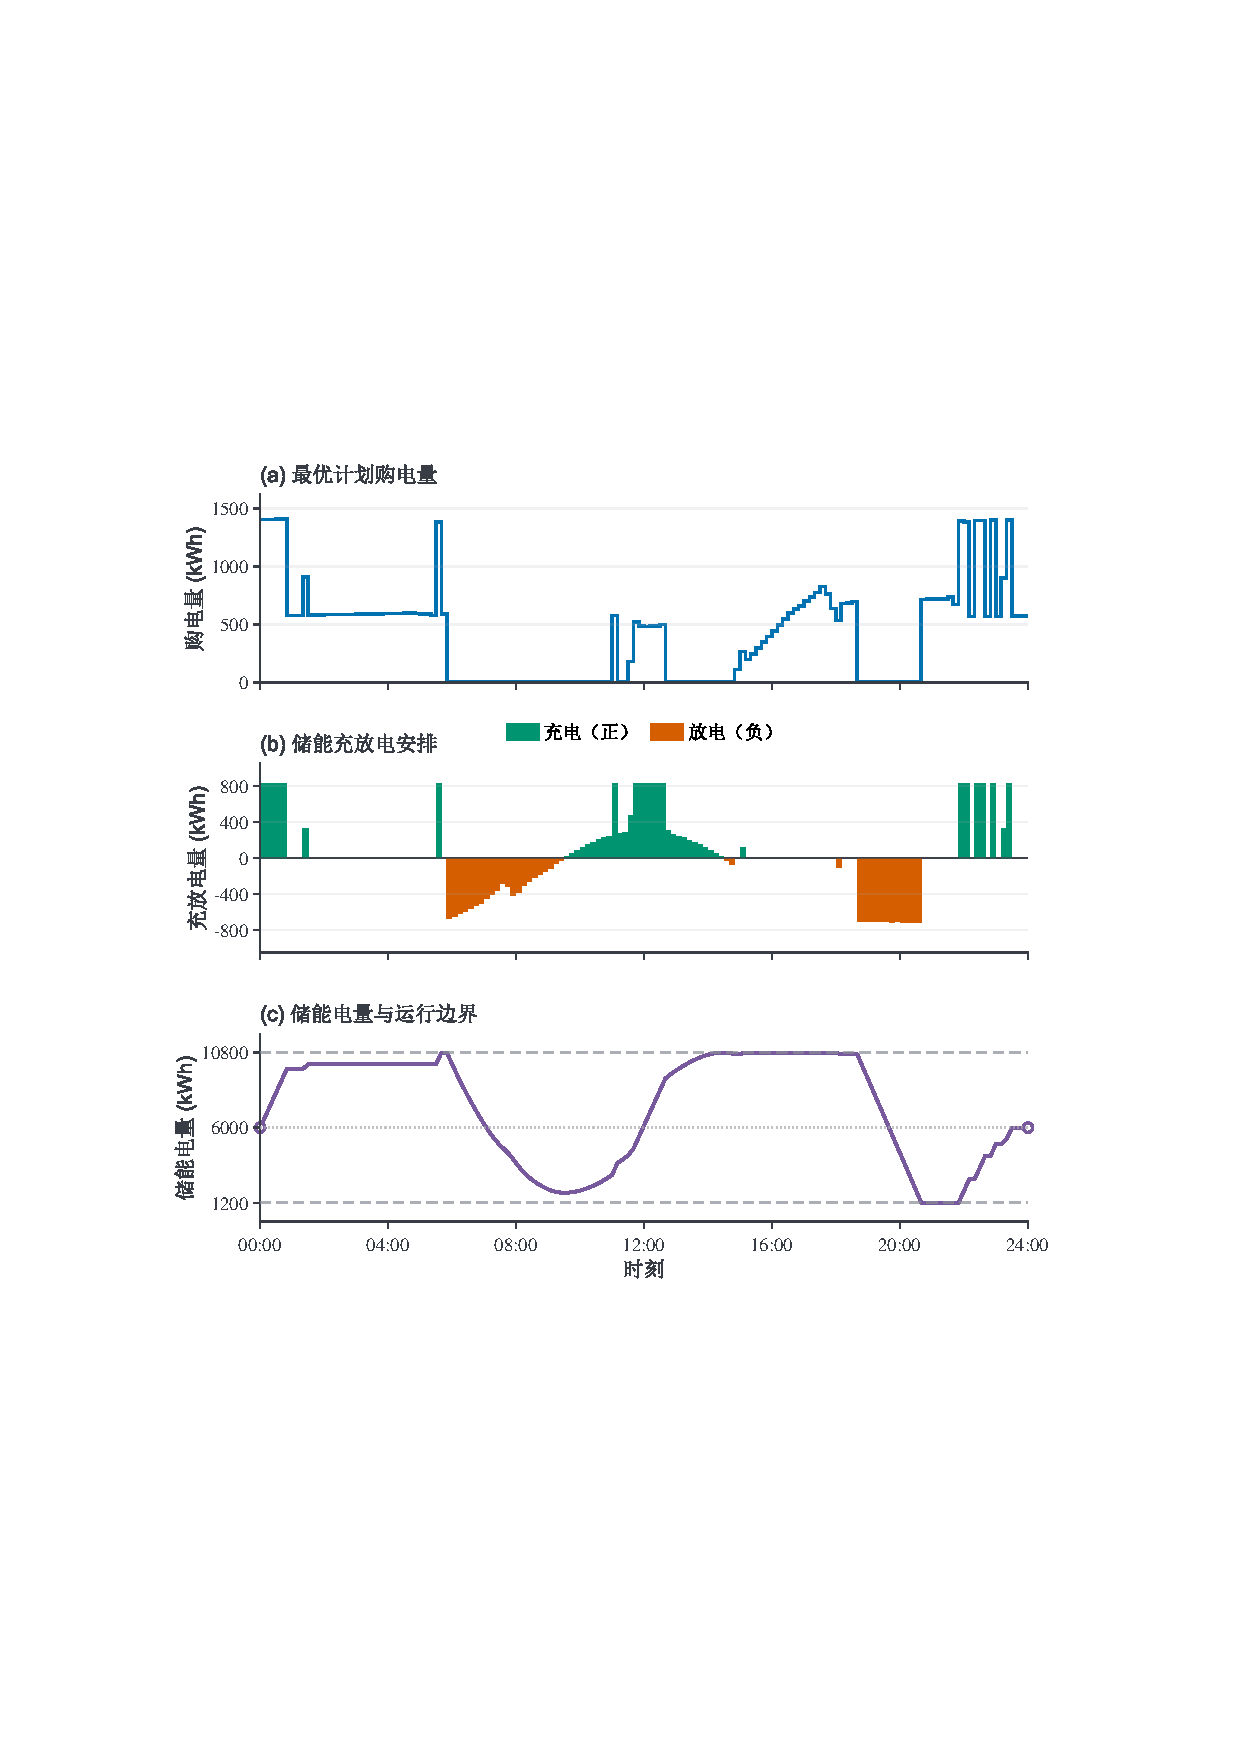
\includegraphics[width=0.78\textwidth]{p1_fig2.pdf}
  \caption{最优购电与储能运行策略：计划购电量、储能充放电动作与储电量轨迹}
  \label{fig:q1-strategy}
\end{figure}

\subsubsection{与无储能基准的经济性比较}

无储能基准为逐区间即时平衡：$g_t^{0}=\max(L_t-V_t,0)$。

\begin{table}[H]
  \centering
  \caption{有无储能的经济性比较}
  \label{tab:q1-compare}
  \begin{tabular}{lccc}
    \toprule
    指标 & 无储能 & 有储能 & 变化 \\
    \midrule
    全天购电费 (元) & 48052.0466 & 35126.9486 & $-12925.0980$（节省率 26.90\%） \\
    全天购电量 (kWh) & 61789.9354 & 59482.6990 & $-2307.2364$（$-3.73\%$） \\
    \bottomrule
  \end{tabular}
\end{table}

能量机制与价格机制需分别解释。\textbf{能量机制}：储能充入 20740.6661 kWh、放出 16799.9396 kWh，往返损耗达 3940.7266 kWh；结合购电量减少 2307.2364 kWh，全天能量平衡意味着供能余量减少约 6247.96 kWh——储能吸收的富余供能超过自身损耗，购电量因此净下降。\textbf{价格机制}：按充放电量加权，放电替代电价约 1.1376 元/kWh、充电支付电价约 0.4930 元/kWh，比值约 2.31，大于往返效率决定的盈亏平衡比 $1/(\eta_c\eta_d)=1/0.81\approx1.23$，可见时段转移在存在能量损耗的条件下仍然盈利。

\subsubsection{容量与功率的敏感性分析}
\label{sec:q1-sens}

采用固定下限 1200 kWh、抬升储能上限的放宽路径（图~\ref{fig:q1-sens}a）：扩容右侧差分 $MV_+(h)=\left[C(E_{\max})-C(E_{\max}+h)\right]/h$ 在 $h=60,120,480$ kWh 时均为 0.6550 元/(kWh·日)，$h=1200$ kWh 时为 0.6539，价值函数在该区间接近线性：可用窗口从 9600 增至 10800 kWh，单日费用下降 784.68 元，区间平均扩容收益约 \textbf{0.6539 元/(kWh·日)}。功率上限从 5000 kW 翻倍至 10000 kW，费用仅下降 \textbf{0.47\%}（图~\ref{fig:q1-sens}b）。

\begin{figure}[H]
  \centering
  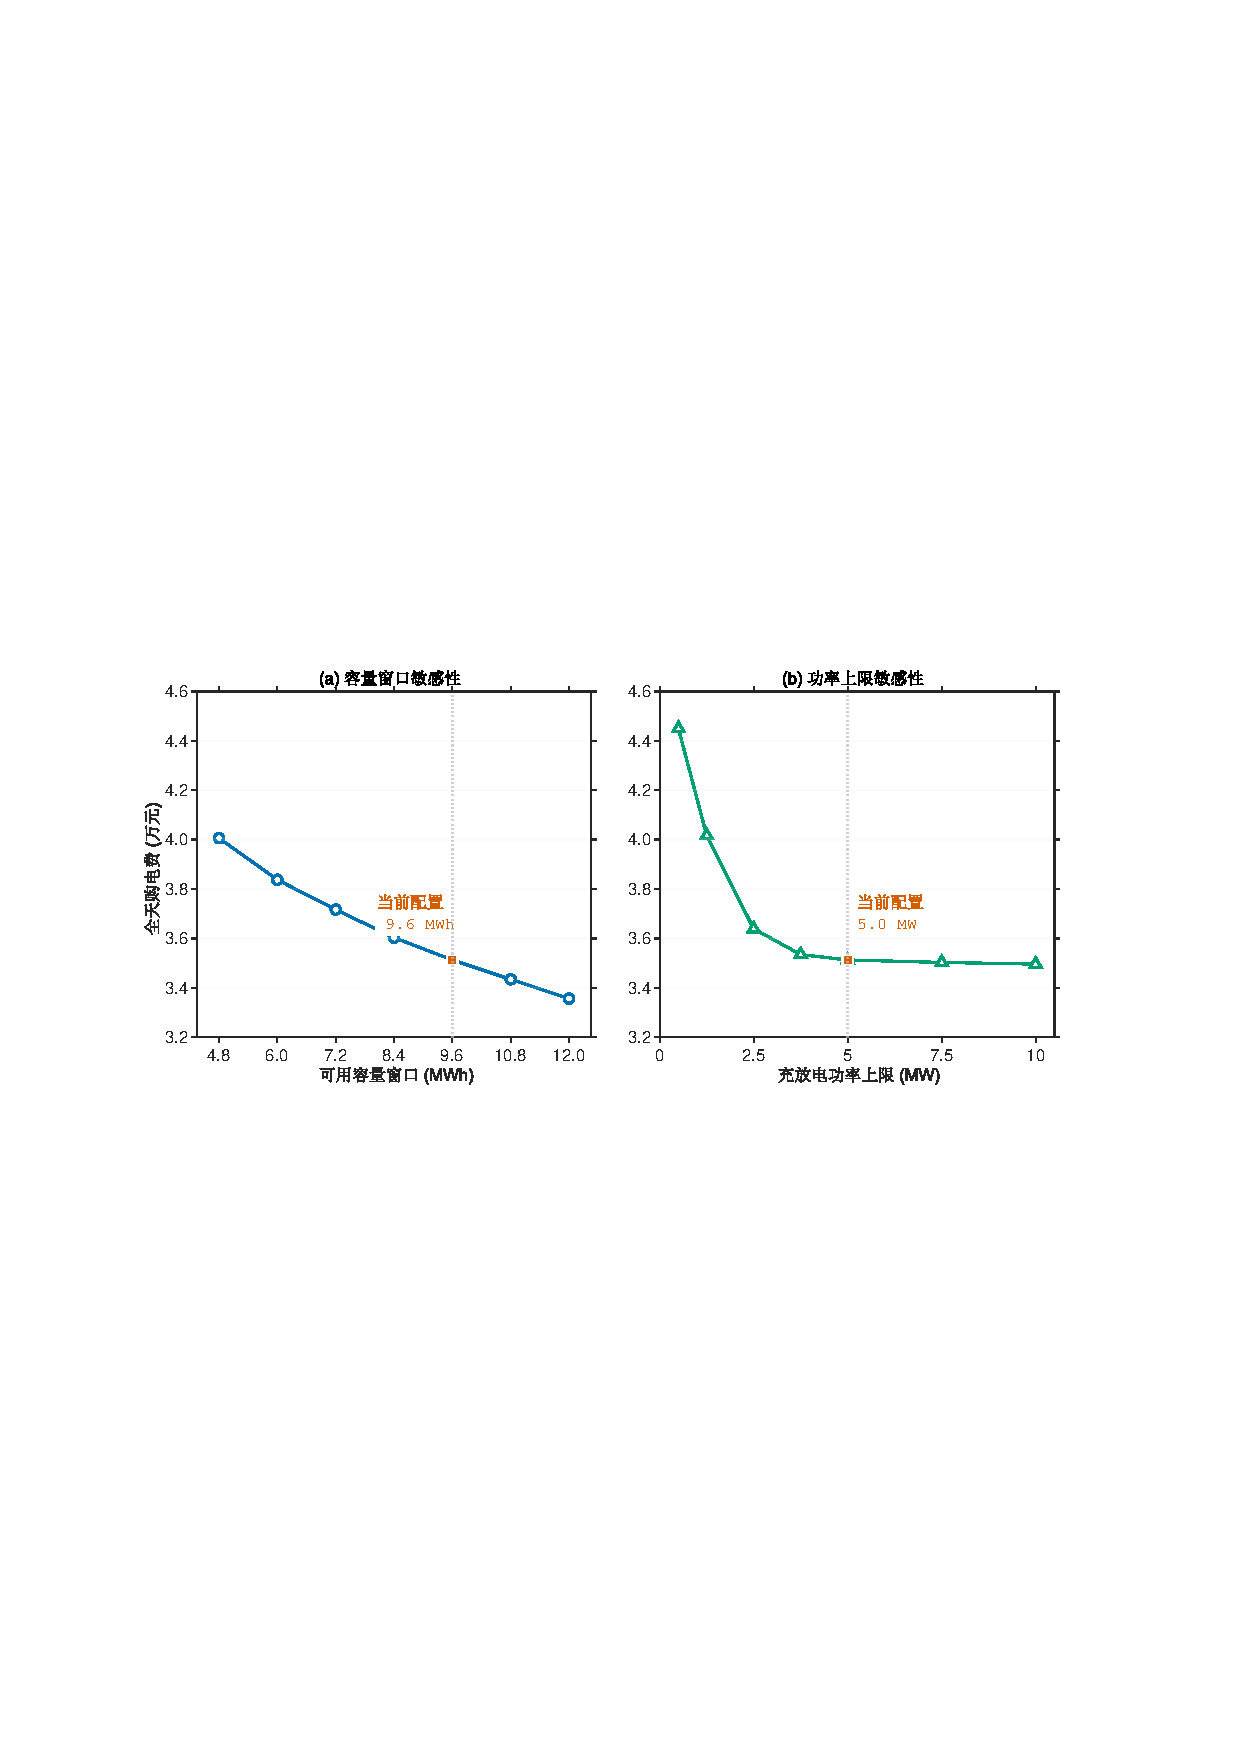
\includegraphics[width=0.88\textwidth]{p1_fig3.pdf}
  \caption{容量窗口与功率上限的敏感性（保持 $E_0=E_{144}=6000$ kWh）}
  \label{fig:q1-sens}
\end{figure}

\textbf{小结}：在本日数据与所考察的约束放宽路径下，容量窗口扩大的降费空间比继续提升充放电功率更为明显。需注意``元/kWh''与``元/kW''量纲不同，不能直接以数值大小比较两类投资的优先级；单日调度收益可为容量配置的讨论提供参考，但不足以单独证明投资合理性。

% =========================================================================
% 五、问题二：序贯决策模型
% =========================================================================

\section{问题二：不确定条件下序贯决策模型的建立与求解}

\subsection{三层滚动决策框架}
\label{sec:q2-frame}

每天 0:00 起依次完成三步（图~\ref{fig:q2-frame}）：
\begin{enumerate}
  \item \textbf{预测层}（\S\ref{sec:q2-forecast}）：由历史实测构造当天净负载预测 $\widehat N_t^{(d)}$；
  \item \textbf{计划层}（\S\ref{sec:q2-lp}）：以 $\widehat N^{(d)}$ 与日初电量 $E_0^{(d)}$ 求解日计划线性规划，输出计划购电量 $b_t$（提交结算）与计划充电意图 $c_t$（执行参考）；
  \item \textbf{执行层}（\S\ref{sec:q2-exec}）：日内按实测 $N_t^{(d)}$ 逐区间实现物理平衡，尽限充放电，不足部分紧急购电；日末电量 $E_H^{(d)}$ 成为次日日初电量 $E_0^{(d+1)}$。
\end{enumerate}
费用按 \S\ref{sec:q2-exec} 的口径逐日结算，全年评价。核心程序见附录~\ref{app:q2-code}。

\begin{figure}[H]
  \centering
  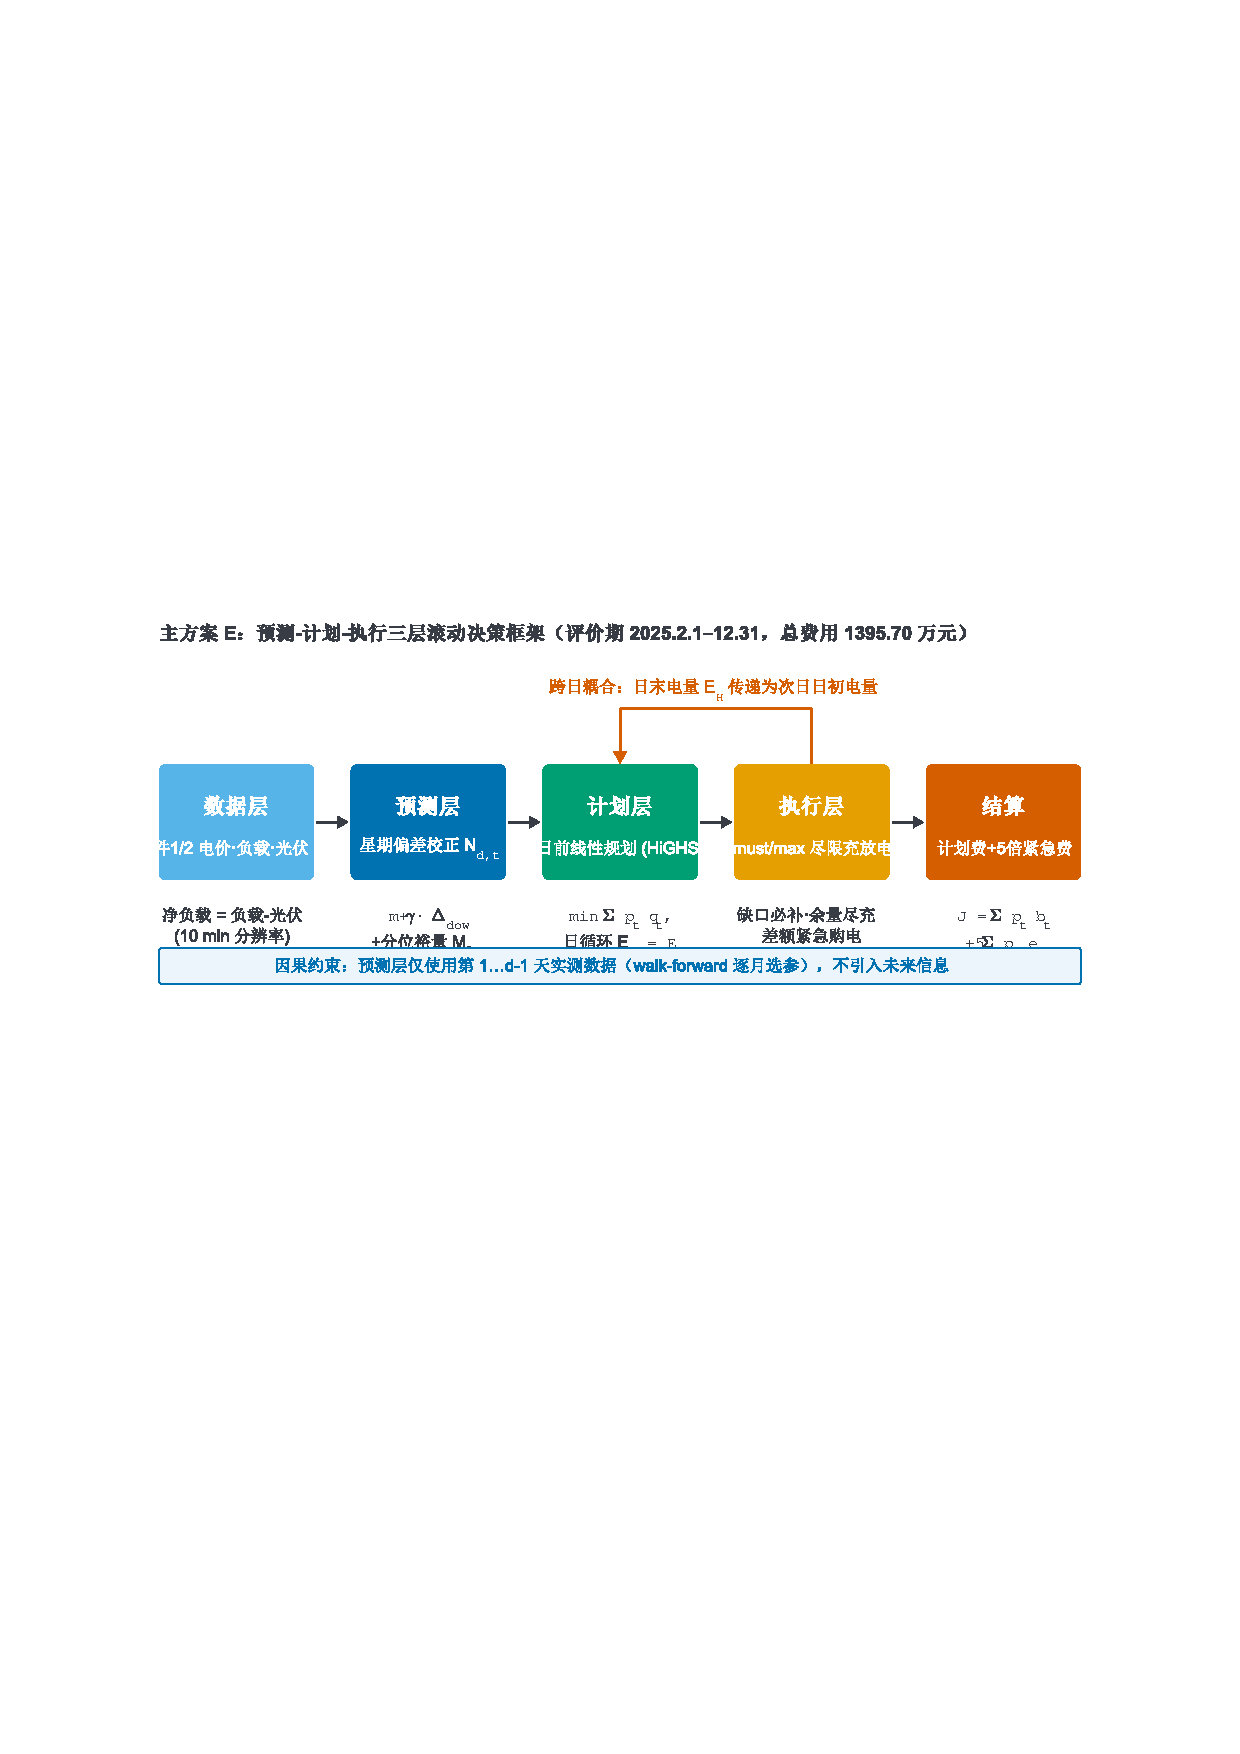
\includegraphics[width=0.9\textwidth]{p2_fig1.pdf}
  \caption{主方案 E 的``预测—计划—执行''三层滚动决策框架}
  \label{fig:q2-frame}
\end{figure}

\subsection{预测层：星期偏差校正的分布预测}
\label{sec:q2-forecast}

预测由三项相加构成：
\begin{equation}
  \widehat N_{d,t}\;=\;\underbrace{m^{\mathrm{r}}_{d,t}}_{\text{近期水平}}\;+\;\underbrace{\gamma\cdot\Delta^{\mathrm{w}}_{d,t}}_{\text{星期偏差校正}}\;+\;\underbrace{M_{\beta,t}}_{\text{分位裕量}} .
  \label{eq:q2-forecast}
\end{equation}

\textbf{（一）近期水平。}取 $d$ 之前最近 $W$ 天实测净负载在时段 $t$ 上的中位数：
\begin{equation}
  m^{\mathrm{r}}_{d,t}=\operatorname*{median}_{s\in[d-W,\;d)}\; N_t^{(s)} .
\end{equation}
用中位数而非均值，是为了对极端天气日稳健；$W$ 反映``水平记忆''的长度，过短则噪声大，过长则跟不上季节漂移。

\textbf{（二）星期偏差。}记 $w(d)\in\{0,\dots,6\}$ 为 $d$ 的星期序号，取 $d$ 之前最近的 $N_{\mathrm{DOW}}$ 个满足 $w(s)=w(d)$ 的日期，对每一天计算``当日实测减当日近期水平''，再取平均：
\begin{equation}
  \Delta^{\mathrm{w}}_{d,t}=\frac{1}{|\mathcal S_d|}\sum_{s\in\mathcal S_d}\Bigl(N_t^{(s)}-m^{\mathrm{r}}_{s,t}\Bigr),\qquad
  \mathcal S_d=\{s<d:\ w(s)=w(d)\}\ \text{中最近的 } N_{\mathrm{DOW}} \text{ 个}.
\end{equation}
这一项刻画``该星期几相对其近期水平的系统性日内形状偏移''；以``实测减该日近期水平''归一化是为了剔除季节漂移。$\gamma\in[0,1]$ 为校正强度，$\gamma=0$ 即退化为不含星期校正的纯水平预测。图~\ref{fig:q2-forecast} 以一个演示周为例展示了式~\eqref{eq:q2-forecast} 各分量的贡献与星期偏差修正项的形态。

\textbf{（三）分位裕量。}前两项只给出条件中心趋势，残余随机波动仍以 5 倍价惩罚。对每个时段 $t$ 单独取近期残差的 $\beta$ 上尾分位数：
\begin{equation}
  M_{\beta,t}=\max\Bigl\{\,Q_\beta\bigl\{N_t^{(s)}-m^{\mathrm{r}}_{s,t}-\gamma\Delta^{\mathrm{w}}_{s,t}\bigr\}_{s\in[d-W,\,d)},\ 0\Bigr\} .
\end{equation}
取 $\max\{\cdot,0\}$ 是为了避免负预留导致系统性的少计划。其经济逻辑与报童模型一致~\cite{newsvendor}：单位低估代价（$5p$ 与触发概率之积）远大于单位高估代价（$p$），最优计划量应落在需求分布的某个上分位数。单时段简化情形下临界分位数为 $5p/(5p+p)=0.83$；但储能提供跨时段物理缓冲，改变了边际代价结构，$\beta$ 不直接套用理论值，而由回放择优（\S\ref{sec:q2-walkforward}）。

\textbf{（四）冷启动回退。}当 $d<30$（1 月内）时，历史不足以估计上述三项，预测器整体回退为附件 1 的代表日净负载曲线；辅助的中位数函数在可用历史不足 7 天时返回零向量，此时预测器已由上一规则回退，不会使用该零向量。

\begin{figure}[H]
  \centering
  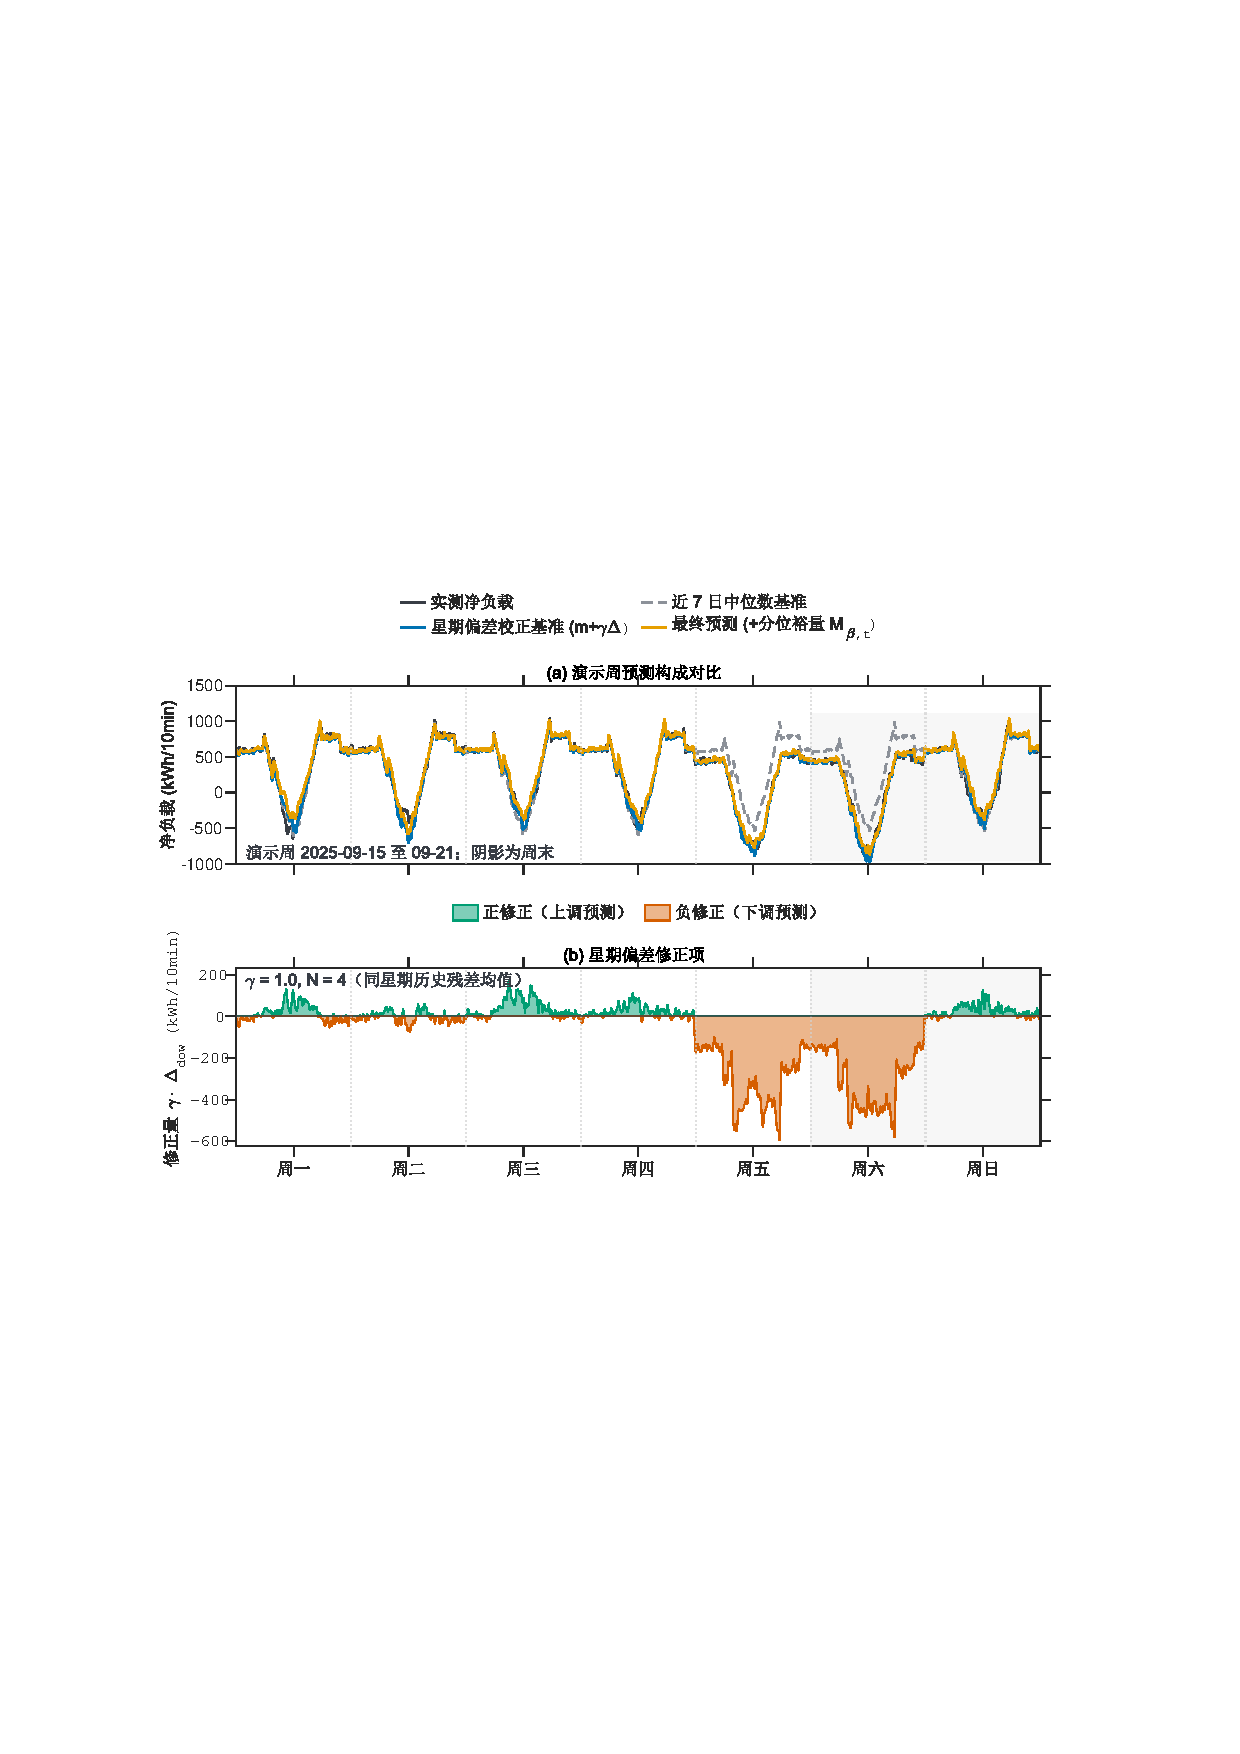
\includegraphics[width=0.85\textwidth]{p2_fig2.pdf}
  \caption{预测构成示例：(a)~演示周内预测各分量对比；(b)~星期偏差修正项}
  \label{fig:q2-forecast}
\end{figure}

\subsection{参数选取：逐月 walk-forward 协议}
\label{sec:q2-walkforward}

待选参数为四元组 $\theta=(\beta, W, \gamma, N_{\mathrm{DOW}})$。选取协议：
\begin{enumerate}
  \item 构造候选网格 $\beta\in\{0.70,0.75\}$，$W\in\{7,14\}$，$\gamma\in\{0,0.5,1.0\}$，$N_{\mathrm{DOW}}\in\{4,6,10\}$，共 36 个候选；
  \item 每个候选全年独立回放一次（从 1 月 1 日 6000 kWh 起连续滚动，得到逐日累计费用序列）；
  \item 第 $m$ 月（$m=2,\dots,12$）使用的参数，取截至 $m-1$ 月月末累计费用最小的候选：
  \begin{equation}
    \theta^{\ast}_m=\arg\min_{\theta}\; J^{(\theta)}_{\le\,\text{月末}(m-1)} .
  \end{equation}
\end{enumerate}
因此参数\textbf{逐月更新}，而非在 1 月一次选定后全年冻结。

\textbf{冷启动期的信息量限制（必须说明）。}由于 $d<30$ 时所有候选共用同一条回退预测，各候选在 1 月 1--30 日的逐日费用完全相同；2 月首次选参时，区分候选的费用信息实际上只来自 1 月 31 日单日。该局限源于算法定义本身，本文不以事后调参加以掩盖；3 月及以后各月可用历史不少于 30 天，选参信息量随之增加。

逐月选出的日程见表~\ref{tab:q2-sched}：11 个月一致地选中 $\gamma=1.0$（完全采用星期偏差校正）与 $N_{\mathrm{DOW}}=4$；$\beta$ 在 2--3 月为 0.70、4 月起为 0.75；$W$ 全程为 7。

\begin{table}[H]
  \centering
  \caption{逐月 walk-forward 选出的参数日程}
  \label{tab:q2-sched}
  \begin{tabular}{lccccccccccc}
    \toprule
    月份 & 2 & 3 & 4 & 5 & 6 & 7 & 8 & 9 & 10 & 11 & 12 \\
    \midrule
    $\beta^\ast$ & 0.70 & 0.70 & 0.75 & 0.75 & 0.75 & 0.75 & 0.75 & 0.75 & 0.75 & 0.75 & 0.75 \\
    $W^\ast$ & 7 & 7 & 7 & 7 & 7 & 7 & 7 & 7 & 7 & 7 & 7 \\
    $\gamma^\ast$ & 1.0 & 1.0 & 1.0 & 1.0 & 1.0 & 1.0 & 1.0 & 1.0 & 1.0 & 1.0 & 1.0 \\
    $N_{\mathrm{DOW}}^\ast$ & 4 & 4 & 4 & 4 & 4 & 4 & 4 & 4 & 4 & 4 & 4 \\
    \bottomrule
  \end{tabular}
\end{table}

\textbf{关于网格边界}：$\gamma=1.0$ 与 $N_{\mathrm{DOW}}=4$ 均位于本文网格边界上。对 $\gamma$，另设置上界扩展至 1.5 的网格（147 个候选），未改变选择结果；对 $N_{\mathrm{DOW}}$，另设置加密网格（28 个候选），所得费用略高 0.79 万元。这些结果只表明``在本文所考察的网格上未发现更优点''，\textbf{不构成全局最优性的证明}。

\subsection{计划层：日循环线性规划}
\label{sec:q2-lp}

给定预测 $\widehat N_t$ 与日初电量 $E_0^{(d)}$，计划层求解：
\begin{align}
  \min\ & \sum_{t=0}^{H-1} p_t\, b_t \\
  \text{s.t.}\quad
  & b_t+d_t=\widehat N_t+c_t+w_t,\qquad E_{t+1}=E_t+\eta_c c_t-\frac{d_t}{\eta_d}, \\
  & E_{\min}\le E_t\le E_{\max},\qquad 0\le c_t,d_t\le \tfrac{5000}{6},\qquad b_t,w_t\ge 0,\qquad \widehat E_H=E_0^{(d)} .
\end{align}
末式为\textbf{日循环约束}：计划轨迹的末端电量等于当日日初电量。两点说明：
\begin{enumerate}
  \item 计划层不含紧急购电项，因为计划必须自足；紧急购电只发生在执行层；
  \item \textbf{日循环仅为计划层的边界条件，不构成对实际运行的约束。}实际 $E_H^{(d)}$ 由执行层按实测决定，可以高于或低于 $E_0^{(d)}$，并自然结转至次日。本文计划层不设任何期末下限。
\end{enumerate}
问题一关于充放电互斥松弛精确性的命题在此同样成立（目标系数非负结构不变），无需引入二元变量。

\subsection{执行层：尽限充放电与结算}
\label{sec:q2-exec}

\textbf{尽限充放电规则。}逐区间比较计划供能 $b_t$ 与实测 $N_t^{(d)}$，令 $\mathrm{net}=b_t-N_t^{(d)}$：
\begin{itemize}
  \item $\mathrm{net}\ge0$（有盈余）：在储能可充空间、功率上限与计划充电意图之内\textbf{尽可能充入}，余量为弃置 $w_t$；
  \item $\mathrm{net}<0$（有缺口）：在储能可放空间与功率上限之内\textbf{尽可能放出}，仍不足的部分即为紧急购电 $e_t$。
\end{itemize}
该规则在有缺口时即时释放可用电量，可直接降低 5 倍电价的紧急购电量；且完全因果，仅使用当前区间的实测值与当前储电量。执行层不允许以普通电价补购未计划电量，与题意的结算口径一致。

\textbf{跨日衔接。}日末电量 $E_H^{(d)}$ 直接成为次日日初电量 $E_0^{(d+1)}$，全年连续；评价期 2 月 1 日统一从 10800 kWh 起评。

\textbf{结算。}第 $d$ 天费用为
\begin{equation}
  J^{(d)}=\sum_{t}p_t\,b_t^{(d)}\;+\;\sum_{t}5p_t\,e_t^{(d)} ,
  \label{eq:q2-cost}
\end{equation}
第一项为计划费（按计划购电量全额结算，无论是否消纳），第二项为紧急费（按交易时刻电价的 5 倍）。两项\textbf{分别核算}：$b_t$ 与 $e_t$ 是物理上不同的两笔电量，不可合并计算。全年指标为评价期 334 天费用之和。

\subsection{完美信息参照方案（不可实施）}

为标定``信息约束''这一项的价值，设一个\textbf{不可实施}的参照方案：物理模型、结算规则、计划层日循环、执行层尽限充放电、起评电量 10800 kWh、评价期 334 天全部与主方案相同，唯一差别是把计划层的 $\widehat N$ 换成当天实测净负载（即日内先知）。其评价期费用为 \textbf{1229.10 万元}（紧急费用为 0）。该参照并非主方案费用的下界（它同样受日循环约束，且预测器不同），仅用于表明``在本文的物理与结算口径下，信息完全时的费用水平''。

\subsection{求解流程与数值校验}

主方案全部结果由 \texttt{scripts/q2\_finalize\_E.py} 一条命令复现：① 读取附件 1/2 并折算电量口径；② 按 \S\ref{sec:q2-walkforward} 逐月取参数 $\to$ \S\ref{sec:q2-forecast} 预测 $\to$ \S\ref{sec:q2-lp} 计划层线性规划 $\to$ \S\ref{sec:q2-exec} 执行层仿真；③ 逐日记录 $b,c,d,e,w,E$；④ 写出 \texttt{result2.xlsx} 与指定日期的三张表。

\textbf{执行器自洽性检查}：将``实测净负载''设为计划所用预测序列时，执行器应精确复现线性规划给出的计划。实测紧急购电总量 $1.1\times10^{-13}$ kWh、充/放电偏差 $<5\times10^{-13}$ kWh、末端储电量偏差为 0，说明计划—执行衔接无结构性损失。

\textbf{全程校验}（评价期）：能量平衡最大残差 $\le1.2\times10^{-13}$ kWh；储电量全程位于 $[1200,10800]$；跨日储电量断裂为 0（次日日初严格等于上一日日末）；计划费与紧急费独立复算一致。主方案评价期总费用 1395.6995 万元由选参、风险档案、提交表三条独立路径各自复算，\textbf{逐位一致}。

% =========================================================================
% 六、问题二的结果分析
% =========================================================================

\section{问题二的结果分析}

结果分析按``总体—分日—风险—对照''四个层次展开：先给出评价期总体结果（\S\ref{sec:q2-total}），再分析指定日期的调度细节（\S\ref{sec:q2-days}），继而讨论全年运行形态与逐月费用（\S\ref{sec:q2-year}）以及紧急购电与风险结构（\S\ref{sec:q2-risk}），最后通过对照方案与消融实验定位各项机制的价值（\S\ref{sec:q2-ablation}）。

\subsection{评价期总费用与构成}
\label{sec:q2-total}

\begin{table}[H]
  \centering
  \caption{主方案评价期结果（2025.2.1--12.31，334 天，起评 10800 kWh）}
  \label{tab:q2-total}
  \begin{tabular}{lc}
    \toprule
    项目 & 数值 \\
    \midrule
    \textbf{总费用} & \textbf{1395.6995 万元} \\
    计划费用 & 1318.2416 万元（94.5\%） \\
    紧急费用 & 77.4578 万元（5.5\%） \\
    计划购电量 & 2165.26 万 kWh \\
    紧急购电量 & 12.44 万 kWh \\
    发生紧急购电的天数 & 163 / 334（48.8\%） \\
    弃置供能余量 & 252.63 万 kWh \\
    \bottomrule
  \end{tabular}
\end{table}

紧急费用只占总费用的 5.5\%，紧急电量仅占计划购电量的 0.57\%。这说明星期偏差校正已修正预测的中心趋势，分位裕量（$\beta=0.75$）足以吸收绝大部分残余波动，5 倍电价惩罚仅在少数时段被触发。

\subsection{指定日期的调度结果}
\label{sec:q2-days}

\begin{figure}[H]
  \centering
  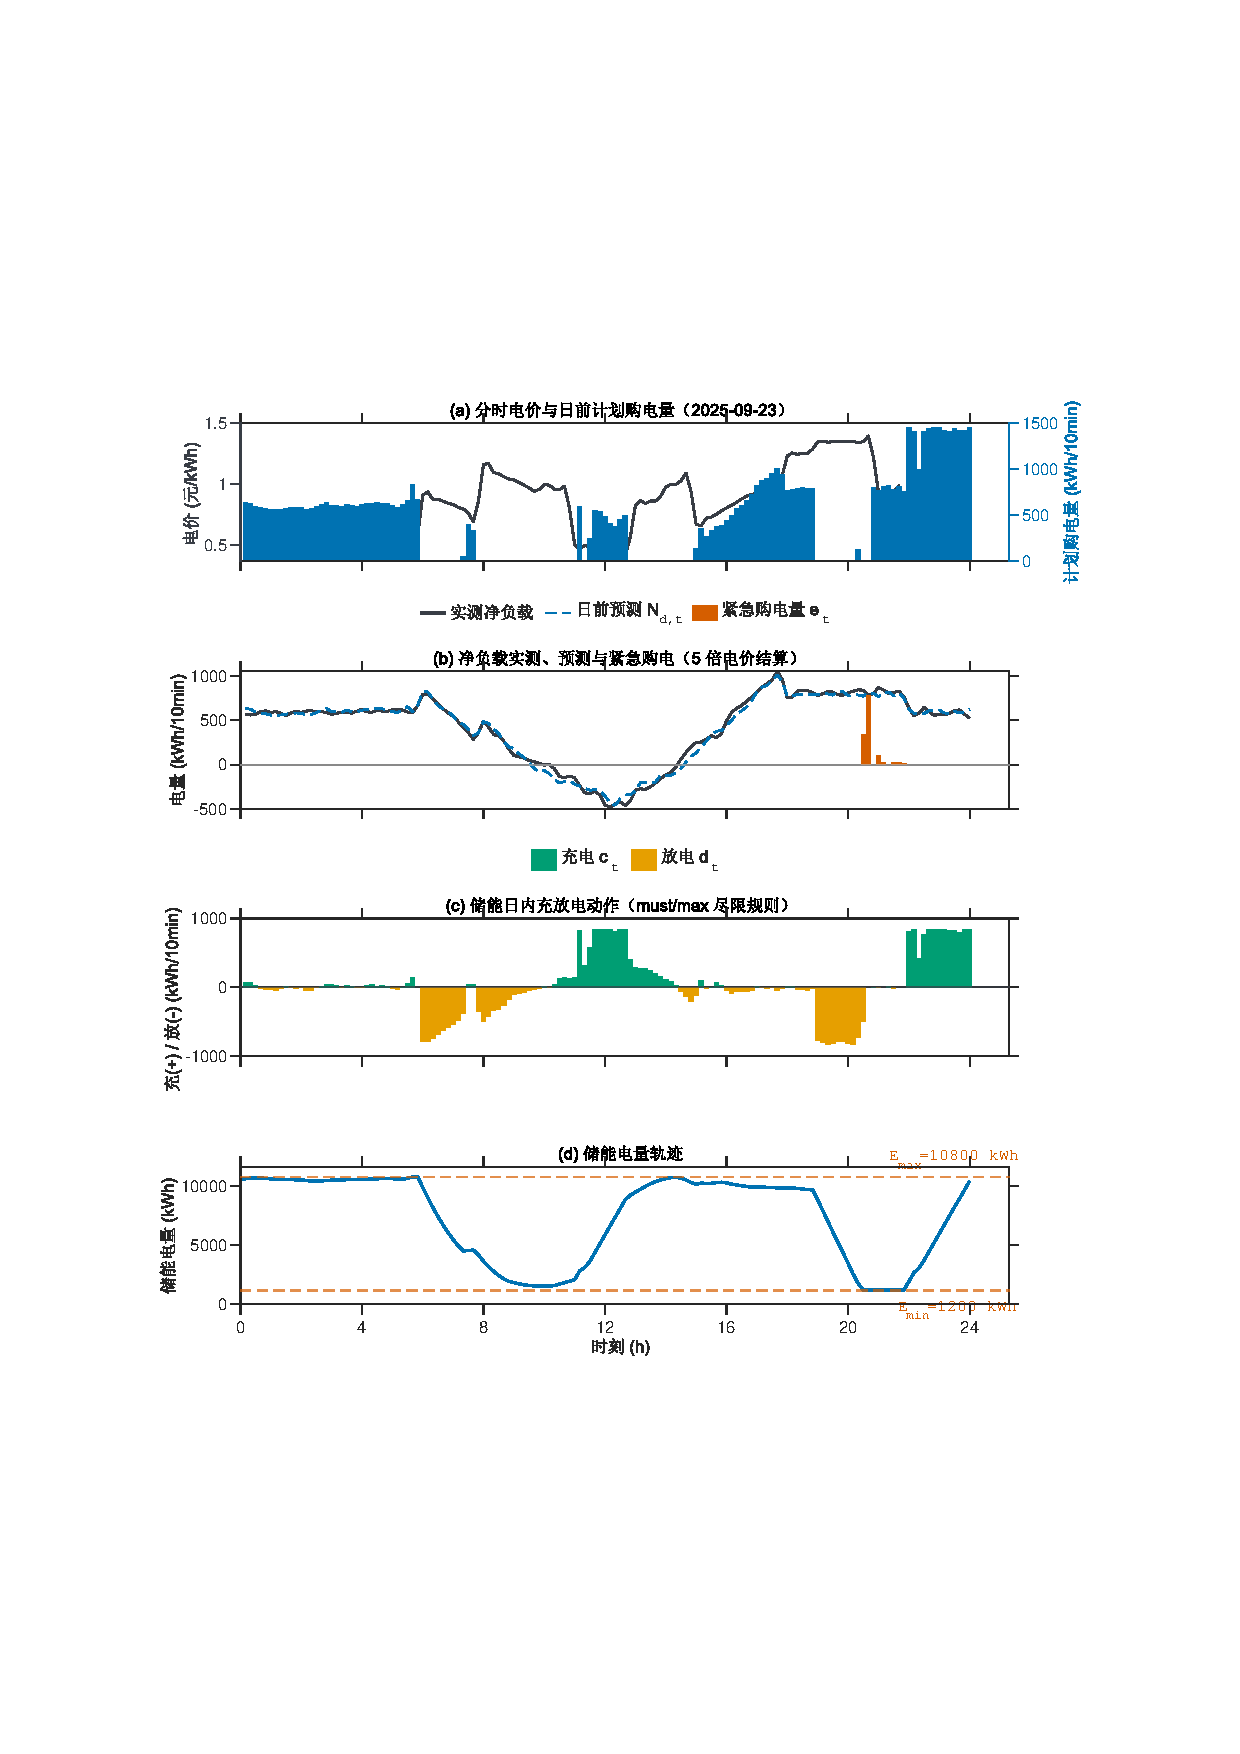
\includegraphics[width=0.86\textwidth]{p2_fig3.pdf}
  \caption{指定日期的调度细节：(a)~分时电价与日前计划购电量；(b)~净负载实测、预测与紧急购电；(c)~储能日内充放电动作；(d)~储能电量轨迹}
  \label{fig:q2-days}
\end{figure}

下列数值按字面时钟区间报告；\texttt{result2.xlsx} 按官方模板原始行序逐行填写、未改动模板标签（模板行标签较字面区间整体后移一个区间），两口径相差一个 10 分钟区间，核对时需注意。

\begin{table}[H]
  \centering
  \caption{指定日期的计划购电量（对应题目表 1 的指定时间段，kWh）}
  \label{tab:q2-t1}
  \small
  \setlength{\tabcolsep}{5pt}
  \begin{tabular}{|c|c|c|c|c|}
    \hline
    时间段 & 2025-03-20 & 2025-06-21 & 2025-09-23 & 2025-12-21 \\ \hline
    10:00--10:10 & 0.0000 & 0.0000 & 0.0000 & 0.0000 \\ \hline
    12:00--12:10 & 545.0194 & 0.0000 & 406.6138 & 1042.1389 \\ \hline
    14:00--14:10 & 0.0000 & 0.0000 & 0.0000 & 0.0000 \\ \hline
    16:00--16:10 & 512.0462 & 224.7427 & 499.3924 & 852.9497 \\ \hline
    18:00--18:10 & 701.8570 & 0.0000 & 772.4848 & 735.2130 \\ \hline
    20:00--20:10 & 0.0000 & 0.0000 & 0.0000 & 0.0000 \\ \hline
  \end{tabular}
\end{table}

\begin{table}[H]
  \centering
  \caption{指定日期的全天购电量（kWh）与费用汇总（对应题目表 1 的汇总行）}
  \label{tab:q2-daysum}
  \small
  \setlength{\tabcolsep}{5pt}
  \begin{tabular}{|c|r|r|r|r|}
    \hline
    日期 & 计划购电量 & 紧急购电量 & 合计购电量 & 费用 (元) \\ \hline
    2025-03-20 & 67872.0855 & 293.0319 & 68165.1174 & 43077.5075 \\ \hline
    2025-06-21 & 36887.8821 & 0.0000 & 36887.8821 & 20795.3006 \\ \hline
    2025-09-23 & 65531.4200 & 1317.0219 & 66848.4419 & 49169.8748 \\ \hline
    2025-12-21 & 98705.7213 & 0.0000 & 98705.7213 & 63439.8523 \\ \hline
  \end{tabular}
\end{table}

表中``全天计划购电量''为 $b_t$ 全天之和，\textbf{不含}紧急购电量；``合计购电量''为两者之和；全天费用＝计划费＋紧急费（式~\eqref{eq:q2-cost}）。

\begin{table}[H]
  \centering
  \caption{指定日期储能设备充放电量（kWh）与日初日末储电量（对应题目表 2）}
  \label{tab:q2-t2}
  \small
  \setlength{\tabcolsep}{4pt}
  \begin{tabular}{|c|c|c|c|c|c|}
    \hline
    时间段 & 充电量 & 放电量 & 时间段 & 充电量 & 放电量 \\ \hline
    \multicolumn{6}{|c|}{2025-03-20} \\ \hline
    0:00--4:00   & 133.3  & 189.8   & 4:00--8:00   & 300.1   & 5166.4 \\ \hline
    8:00--12:00  & 6059.0 & 2777.4  & 12:00--16:00 & 3905.3  & 543.2 \\ \hline
    16:00--20:00 & 234.1  & 5937.8  & 20:00--24:00 & 10717.5 & 2692.8 \\ \hline
    \multicolumn{2}{|c|}{0:00 储电量} & 10800.0000
      & \multicolumn{2}{c|}{24:00 储电量} & 10783.9968 \\ \hline
    \multicolumn{6}{|c|}{2025-06-21} \\ \hline
    0:00--4:00   & 169.8   & 3413.0  & 4:00--8:00   & 384.1   & 4836.6 \\ \hline
    8:00--12:00  & 9630.8  & 0.0000  & 12:00--16:00 & 0.0000  & 0.0000 \\ \hline
    16:00--20:00 & 115.0   & 5727.6  & 20:00--24:00 & 10025.0 & 2485.9 \\ \hline
    \multicolumn{2}{|c|}{0:00 储电量} & 10800.0000
      & \multicolumn{2}{c|}{24:00 储电量} & 10800.0000 \\ \hline
    \multicolumn{6}{|c|}{2025-09-23} \\ \hline
    0:00--4:00   & 330.5  & 288.5   & 4:00--8:00   & 411.2   & 6550.3 \\ \hline
    8:00--12:00  & 4827.1 & 1896.6  & 12:00--16:00 & 5621.7  & 596.0 \\ \hline
    16:00--20:00 & 35.0   & 6159.9  & 20:00--24:00 & 10298.8 & 2061.4 \\ \hline
    \multicolumn{2}{|c|}{0:00 储电量} & 10585.6180
      & \multicolumn{2}{c|}{24:00 储电量} & 10454.3513 \\ \hline
    \multicolumn{6}{|c|}{2025-12-21} \\ \hline
    0:00--4:00   & 94.5   & 172.0   & 4:00--8:00   & 989.4   & 1528.6 \\ \hline
    8:00--12:00  & 6188.6 & 6906.2  & 12:00--16:00 & 6116.1  & 2237.9 \\ \hline
    16:00--20:00 & 0.0000 & 5712.0  & 20:00--24:00 & 10561.2 & 2842.5 \\ \hline
    \multicolumn{2}{|c|}{0:00 储电量} & 10800.0000
      & \multicolumn{2}{c|}{24:00 储电量} & 10800.0000 \\ \hline
  \end{tabular}
\end{table}

四日都呈现``白天光伏充沛时充电、晚峰放电、深夜低谷再充满''的典型日循环形态（图~\ref{fig:q2-days}c、d）；日末与日初电量并不相等（如 09-23 日初 10585.62 $\to$ 日末 10454.35 kWh），体现了实际储电量的跨日连续衔接。

\begin{table}[H]
  \centering
  \caption{指定日期紧急购电结果（对应题目表 3，合并连续区间）}
  \label{tab:q2-t3}
  \small
  \setlength{\tabcolsep}{6pt}
  \begin{tabular}{|c|c|r|}
    \hline
    日期 & 紧急购电时间段 & 紧急购电量 (kWh) \\ \hline
    2025-03-20 & 20:30--20:40 & 293.03 \\ \hline
    2025-06-21 & （无紧急购电） & 0.00 \\ \hline
    2025-09-23 & 20:20--20:40 & 1126.01 \\ \hline
               & 20:50--21:10 & 129.61 \\ \hline
               & 21:20--21:50 & 61.40 \\ \hline
    2025-12-21 & （无紧急购电） & 0.00 \\ \hline
  \end{tabular}
\end{table}

紧急购电集中在晚间光伏退出后的时段（09-23 共 1317.02 kWh，见图~\ref{fig:q2-days}b），与净负载的日内形态一致；06-21 为光伏旺季，计划自足；12-21 为冬季大负载日，计划量充裕。

\subsection{全年运行形态与逐月费用}
\label{sec:q2-year}

\begin{figure}[H]
  \centering
  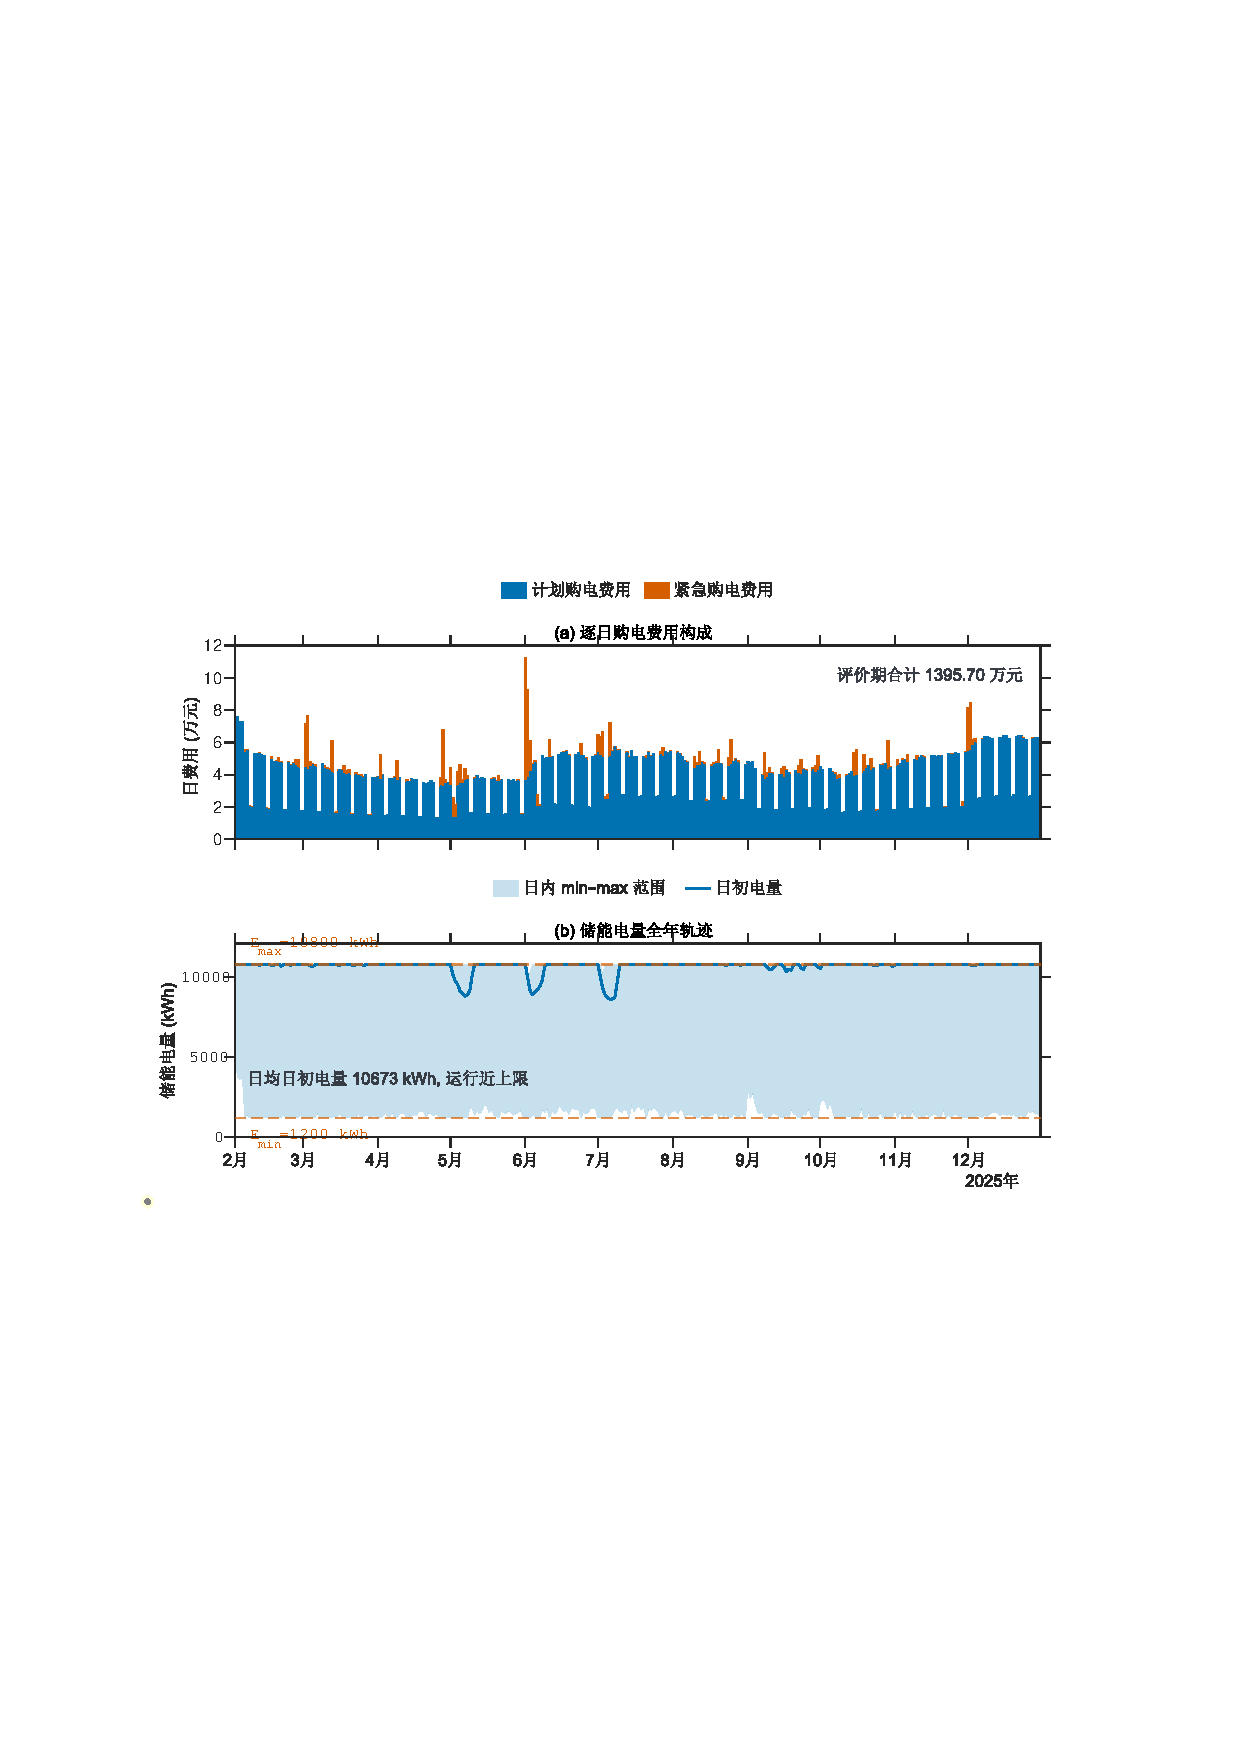
\includegraphics[width=0.9\textwidth]{p2_fig4.pdf}
  \caption{逐日购电费用构成与储能电量全年轨迹}
  \label{fig:q2-year}
\end{figure}

\begin{figure}[H]
  \centering
  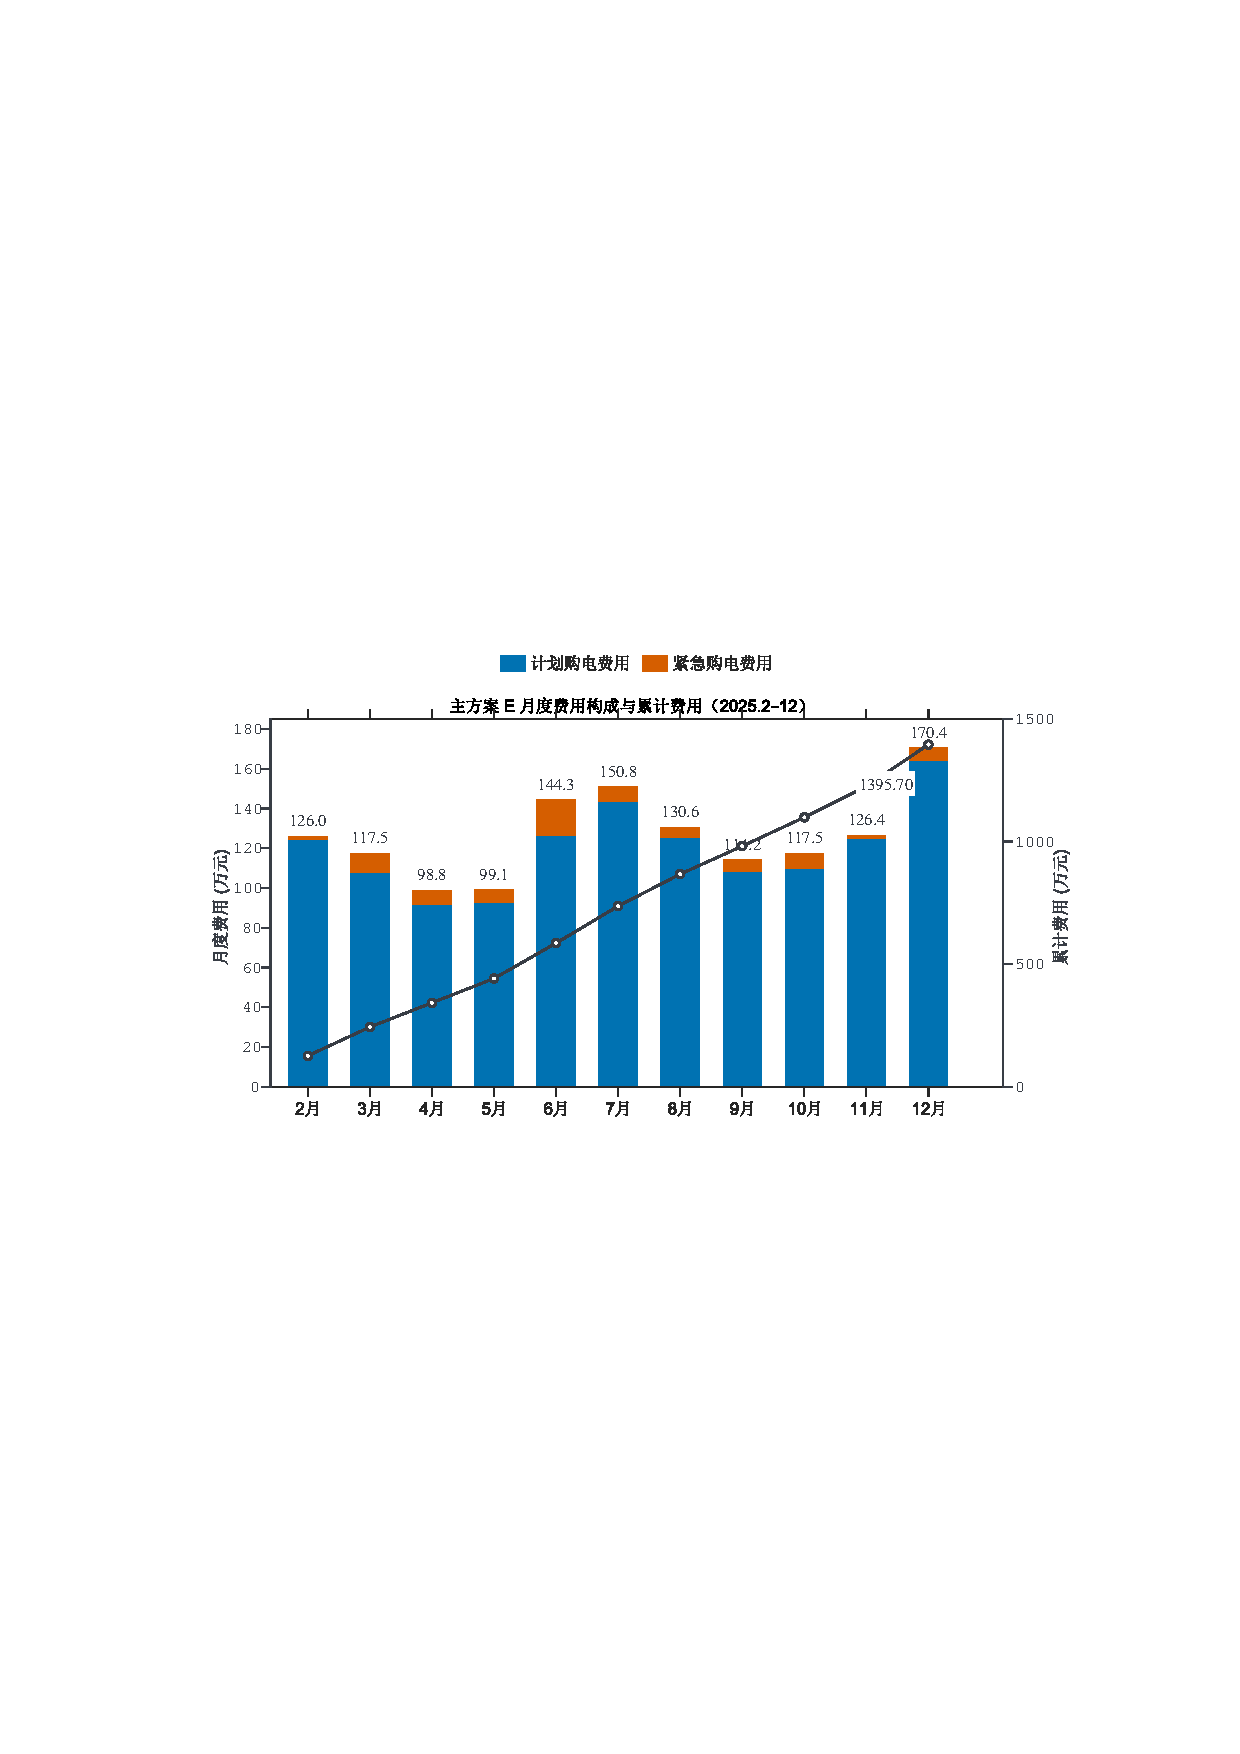
\includegraphics[width=0.88\textwidth]{p2_fig5.pdf}
  \caption{月度费用构成与累计费用}
  \label{fig:q2-month}
\end{figure}

\begin{table}[H]
  \centering
  \caption{主方案月度费用（万元）与风险概况}
  \label{tab:q2-month}
  \begin{tabular}{crcrrr}
    \toprule
    月份 & 总费用 & 计划 & 紧急 & 大紧急天数$^{*}$ & 触顶天数 \\
    \midrule
    2  & 125.96 & 124.23 & 1.74 & 0 & 28 \\
    3  & 117.46 & 107.58 & 9.88 & 3 & 31 \\
    \textbf{4}  & \textbf{98.84}（最低） & 91.75 & 7.09 & 3 & 30 \\
    5  & 99.13 & 92.45 & 6.68 & 6 & 31 \\
    6  & 144.34 & 126.52 & 17.83 & 5 & 28 \\
    7  & 150.79 & 143.39 & 7.40 & 4 & 30 \\
    8  & 130.64 & 125.27 & 5.37 & 4 & 31 \\
    9  & 114.24 & 108.07 & 6.16 & 4 & 28 \\
    10 & 117.45 & 109.96 & 7.49 & 5 & 31 \\
    11 & 126.43 & 124.86 & 1.57 & 0 & 30 \\
    \textbf{12} & \textbf{170.42}（最高） & 164.16 & 6.26 & 2 & 29 \\
    \bottomrule
  \end{tabular}
\end{table}

$^{*}$\ 大紧急天数＝当日紧急购电量超过 1000 kWh 的天数。

12 月费用最高（170.42 万元，冬季大负载、光伏弱，计划购电量最多）；4 月最低（98.84 万元，春季温和、光伏进入旺季）；6 月紧急费用最高（17.83 万元，5 个大紧急日），对应初夏光伏出力波动叠加晚峰缺口，是全年风险最集中的月份（图~\ref{fig:q2-month}）。

\subsection{紧急购电与风险结构}
\label{sec:q2-risk}

\begin{figure}[H]
  \centering
  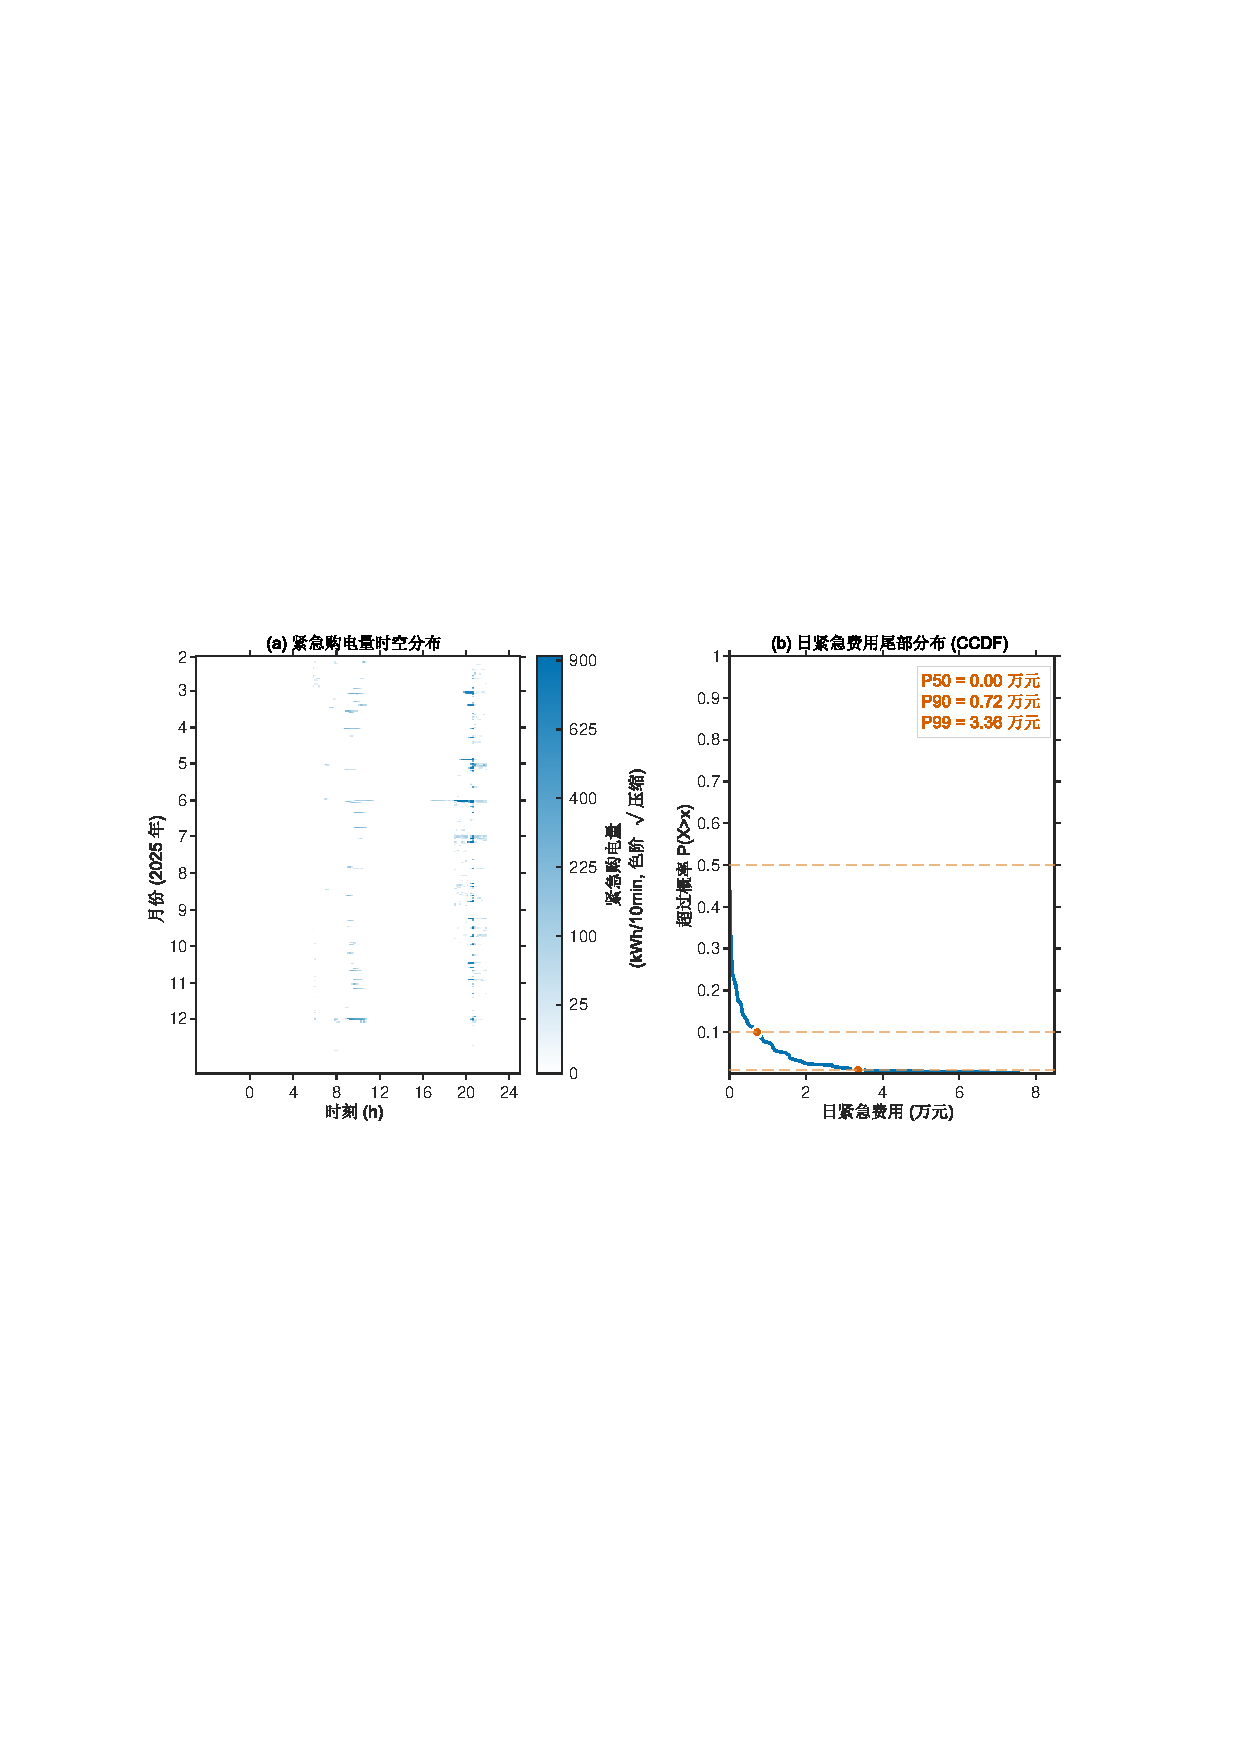
\includegraphics[width=0.9\textwidth]{p2_fig6.pdf}
  \caption{紧急购电特征：(a)~紧急购电量时空分布；(b)~日紧急购电费用分布}
  \label{fig:q2-emerg}
\end{figure}

\begin{table}[H]
  \centering
  \caption{主方案风险指标（评价期 334 天）}
  \label{tab:q2-risk}
  \begin{tabular}{lc}
    \toprule
    指标 & 数值 \\
    \midrule
    紧急费用分位数 P50 / P90 / P95 / P99 & 0.00 / 0.71 / 1.33 / 3.20 万元 \\
    单日最坏紧急费用 & 7.58 万元 \\
    大紧急天数（$>1000$ kWh） & 36 / 334（10.8\%） \\
    触底天数（日内有 $E_t\le E_{\min}$） & 113 / 334（33.8\%） \\
    触顶天数（日内有 $E_t=E_{\max}$） & 327 / 334（97.9\%） \\
    日均起始／日内最低／日内最高储电量 & 10673 / \textbf{1444} / \textbf{10793} kWh \\
    年末储电量（12.31 日末） & 10667 kWh \\
    \bottomrule
  \end{tabular}
\end{table}

\textbf{储备结构的准确表述}：过半数日期（P50＝0）不发生任何紧急购电，尾部风险可控（P99＝3.20 万元，图~\ref{fig:q2-emerg}）。触顶天数 327/334 仅表示这些天日内\textbf{至少一次}达到上限，不等于全天维持满电：日内最低储电量平均 1444 kWh，接近下限 1200 kWh，说明储能每天仍经历一次幅度较大的充放电循环（日均最高 10793 $\to$ 日均最低 1444 kWh）。因此主方案的运行形态是``低谷充满—晚峰放空—再充满''的日循环（图~\ref{fig:q2-year}），而非``长期保持满电''。

\subsection{方案对照与条件消融}
\label{sec:q2-ablation}

本文在建模过程中先后构造了一组递进方案，用于对照不同的预测器与执行规则。它们与主方案共用评价口径（2/1 起评 10800 kWh），但分属不同的模型族，故\textbf{仅作水平对照，不将差额归因于某一单项机制}（图~\ref{fig:q2-ladder}a）。

\begin{table}[H]
  \centering
  \caption{对照方案与主方案的水平比较（评价口径统一）}
  \label{tab:q2-ladder}
  \small
  \begin{tabular}{llcc}
    \toprule
    方案 & 预测方式／执行方式 & 总费用 (万元) & 相对 A \\
    \midrule
    A & 固定代表日曲线／贪心 & 2825.28 & — \\
    B & 代表日＋残差中位数校准／贪心 & 2035.24 & $-28.0\%$ \\
    B48 & B＋48 小时计划窗口／贪心 & 2024.98 & $-28.3\%$ \\
    C & B＋分位裕量（$\beta=0.7$）／贪心 & 1775.91 & $-37.1\%$ \\
    D & C／每 4 小时重优化 & 1739.64 & $-38.4\%$ \\
    \textbf{E（主方案）} & \textbf{近期水平＋星期偏差＋分位裕量}／\textbf{尽限充放电} & \textbf{1395.70} & \textbf{$-50.6\%$} \\
    完美信息参照 & 当天实测（不可实施）／尽限充放电 & 1229.10 & $-56.5\%$ \\
    \bottomrule
  \end{tabular}
\end{table}

\begin{figure}[H]
  \centering
  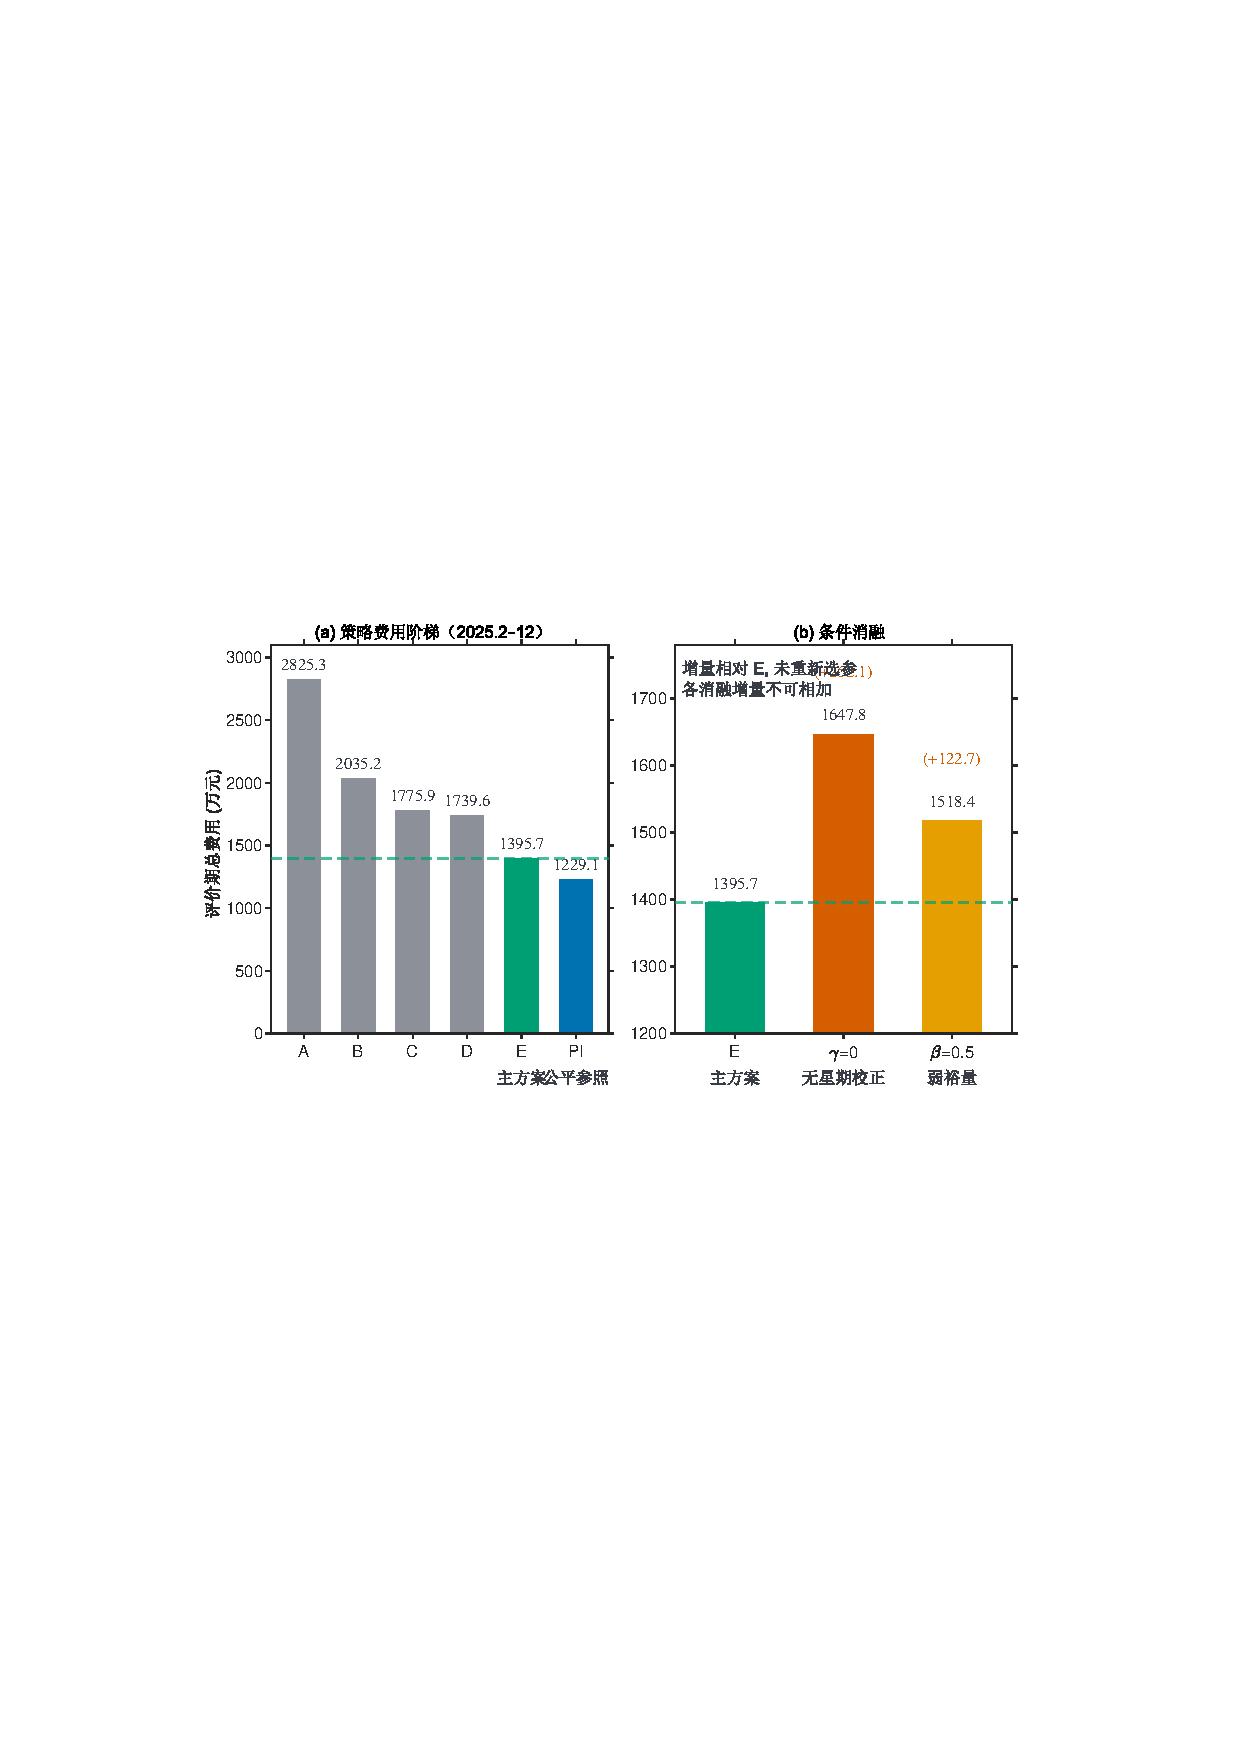
\includegraphics[width=0.9\textwidth]{p2_fig7.pdf}
  \caption{(a)~各方案的评价期总费用阶梯；(b)~条件消融实验}
  \label{fig:q2-ladder}
\end{figure}

\textbf{同链路的单项消融。}为单独识别星期偏差校正的作用，另做``关闭星期偏差''的同链路对照（图~\ref{fig:q2-ladder}b）：保持计划层、执行层、起评电量、$\beta=0.70$、$W=14$ 全部不变，仅令 $\gamma=0$，得 1719.71 万元。与同一链路下 $N_{\mathrm{DOW}}=4$ 的主方案相比，星期偏差校正与逐月联合选参合计带来 \textbf{324.01 万元（$-18.84\%$）}的降幅。该对照中各项设置一致，差额可归因于预测器与选参方式；但两项各自的贡献尚未单独分离。

\textbf{与完美信息参照的差距。}主方案 1395.70 万元，完美信息参照 1229.10 万元，相差 166.60 万元。这一差距不应整体解读为``可改进空间''：① 参照方案同样受日循环约束，若取消该约束其费用只会更低，故 166.60 万元不是严格意义上的信息缺口成本；② 差距中包含天气等不可预测的随机成分，任何因果策略都必须承担这部分代价；③ 5 倍电价的损失不对称使``保险溢价''不可避免——即使预测无偏，最优计划水平也应高于条件中位数。

% =========================================================================
% 七、问题三：滚动合同调整模型
% =========================================================================

\section{问题三：多时刻预报下滚动合同调整模型的建立与求解}

\subsection{信息结构与结算规则}
\label{sec:q3-frame}

问题二只有``计划—执行''两层：0:00 计划一经制定即为结算依据，实测缺口只能按 5 倍价紧急补足。问题三在两点上改变了这一结构：

\begin{enumerate}
  \item \textbf{信息增加}：除 0:00 外，6:00、12:00、18:00 还可获得未来 24 小时整点光伏预报（附件 3），因而日内可以滚动更新对剩余时段光伏出力（进而净负载）的认识；
  \item \textbf{结算增加}：允许在预报时刻\textbf{重新约定}剩余时段的购电量，但双向偏离 0:00 计划都要付费——\textbf{计划高于调整}的差额按 $0.5p_t$ 的违约电价结算，\textbf{调整高于计划}的差额按 $1.5p_t$ 结算；紧急购电仍为 $5p_t$。
\end{enumerate}

由此形成``计划—调整—执行''三层结构：在问题二框架（图~\ref{fig:q2-frame}）的``计划层''与``执行层''之间，插入一个在每个预报时刻重复触发的\textbf{调整层}。此时需定量回答两个问题：\textbf{(i)} 日内调整机会本身的价值；\textbf{(ii)} 在 6:00、12:00、18:00 三个时刻使用预报（而非仅在 0:00 使用一次）是否经济。后者是题面明确要求分析的问题。

\subsection{预报通道与净负载预测}
\label{sec:q3-forecast}

\textbf{（一）整点预报转区间电量。}附件 3 只给出逐日四个发布时刻对未来 24 小时\textbf{整点}的光伏功率预报。记发布时刻为 $\tau\in\{0,6,12,18\}$、其预报曲线为 $f_\tau(h)$，将其在相邻整点间线性插值、再在 10 分钟区间上积分，得区间电量
\begin{equation}
  \widetilde V_t(\tau)=\tfrac12\bigl[f_\tau(\tau_t)+f_\tau(\tau_{t+1})\bigr]\Delta t ,
  \label{eq:q3-pv}
\end{equation}
其中 $\tau_t=t\Delta t$ 为区间起点时刻。$\tau>0$ 时曲线端点以\textbf{当日已实测光伏功率的水平}锚定（而非初值或瞬时值），以削弱插值端点的噪声；$\tau=0$ 通道该时刻尚无实测，端点取零。

\textbf{（二）0:00 通道的预报融合。}问题二预测器所用的光伏分量来自历史经验形状，而附件 3 提供了当日的光伏预报，故可对预测作一步收缩修正：
\begin{equation}
  \widehat N_t \;=\; \underbrace{\bigl(m^{\mathrm{r}}+\gamma\Delta^{\mathrm{w}}+M_\beta\bigr)_t}_{\text{问题二预测器（式~\eqref{eq:q2-forecast}）}}\;-\;\kappa_g\Bigl[\widetilde V_t(0)-\widehat V_t^{\mathrm{hist}}\Bigr],
  \label{eq:q3-fuse}
\end{equation}
$\widehat V_t^{\mathrm{hist}}$ 为问题二预测器隐含的光伏分量，$\kappa_g\in[0,1]$ 为\textbf{分档收缩系数}，按预报时长 $h$ 分三档 $g\in\{[0,6),[6,12),[12,24)\}$。$\kappa_g$ 由\textbf{过去 $K=30$ 天}的因果滚动回归估计：
\begin{equation}
  \kappa_g=\mathrm{clip}\!\left(-\frac{\sum_s r_s x_s}{\sum_s x_s^{2}},\,0,\,1\right),\qquad
  r_s=N^{(s)}-\widehat N^{(s)}_{\text{基准}},\quad x_s=\widetilde V^{(s)}(0)-\widehat V^{(s)}_{\mathrm{hist}} ,
  \label{eq:q3-kappa}
\end{equation}
即用``实测净负载残差''对``两条预报通道的差值''回归；取负号是因为光伏预报上调（$x>0$）意味着净负载下调，截断在 $[0,1]$ 以避免过度修正。样本不足 7 天时取 $\kappa_g=0$，退回问题二预测器。$\kappa_g$ 每日仅用 $d-K,\dots,d-1$ 的数据重估，保持与问题二一致的因果口径。

\subsection{调整层：带双向违约价的剩余时段线性规划}
\label{sec:q3-adjust}

在 $\tau\in\{6,12,18\}$，先按\textbf{当前生效合同}执行完上一段区间，得到该时刻的实测储电量 $E_\tau$；再对剩余区间 $t\ge t_\tau$ 重新求解合同 $b'_t$：
\begin{equation}
\begin{aligned}
  \min\;\; & \sum_{t\ge t_\tau} p_t b'_t \;+\; \tfrac12\!\!\sum_{t\ge t_\tau}\! p_t\,(u_t+v_t) \\
  \text{s.t.}\;\;
  & u_t\ \ge\ b_t^{\mathrm{plan}}-b'_t,\qquad v_t\ \ge\ b'_t-b_t^{\mathrm{plan}},\qquad u_t,\,v_t\ge 0, \\
  & b'_t+d_t\ \ge\ \widehat N_t(\tau)+c_t,\qquad E_{t+1}=E_t+\eta_c c_t-\frac{d_t}{\eta_d},\\
  & E_{\min}\le E_t\le E_{\max},\qquad 0\le c_t,\,d_t\le \tfrac{5000}{6},\qquad b'_t\ge0,\\
  & E_{t_\tau}=E_\tau\ (\text{实测}),\qquad E_H=E_0^{(d)} ,
\end{aligned}
  \label{eq:q3-adjust}
\end{equation}
其中偏差始终对\textbf{0:00 计划} $b^{\mathrm{plan}}$ 计量（而非对上一次合同），故连续两次调整不产生重复计费。末式为计划层的日循环边界，同 \S\ref{sec:q2-lp}。

\textbf{目标函数与题面结算规则的等价性。}式~\eqref{eq:q3-adjust} 只需一次线性规划即可同时表示下调的违约费和上调的加价，无需引入分段逻辑：
\begin{itemize}
  \item 当 $b'_t\le b_t^{\mathrm{plan}}$ 时，题面结算为 $p_tb'_t+\tfrac12p_t\bigl(b_t^{\mathrm{plan}}-b'_t\bigr)$，而 $\tfrac12p_t(u_t+v_t)$ 在该情形下恰取 $u_t=b_t^{\mathrm{plan}}-b'_t$、$v_t=0$，二者完全一致；
  \item 当 $b'_t\ge b_t^{\mathrm{plan}}$ 时，$p_tb'_t+\tfrac12p_t\bigl(b'_t-b_t^{\mathrm{plan}}\bigr)=\tfrac32p_tb'_t-\tfrac12p_tb_t^{\mathrm{plan}}$，正是``超出部分按 1.5 倍、未超出部分按 1 倍''的结果。
\end{itemize}
\textbf{调整层必须自足，不含紧急购电项。}供给约束要求合同与储能放电覆盖预测需求（$b'_t+d_t\ge\widehat N_t(\tau)+c_t$），超出部分弃置。若在调整层中引入紧急购电并按其 5 倍价计入目标，线性规划会把缺口``计划''给紧急购电，从而低估所需的合同量、把风险推给执行层；因此本文的调整层不把紧急购电当作可计划的资源。紧急购电只在执行层按实测缺口发生，费用按 \S\ref{sec:q2-exec} 以 $5p_t$ 单独核算。

\textbf{执行层。}仍采用 \S\ref{sec:q2-exec} 的尽限充放电规则，但以\textbf{最新生效合同}为交付基准；段与段之间实测储电量连续传递，日末电量结转为次日日初电量。评价期、起评储电量（10800 kWh）与问题二完全一致，便于横向比较。

\subsection{两维对照：调整机会与 0:00 预报通道}
\label{sec:q3-matrix}

为把``信息''与``调整机会''两项改进分开计量，构造 $2\times2$ 方案矩阵（图~\ref{fig:q3-matrix}）：是否使用附件 3 的 0:00 预报通道（式~\eqref{eq:q3-fuse}）$\times$ 是否允许日内三次调整。

\begin{table}[H]
  \centering
  \caption{0:00 预报通道 $\times$ 日内调整机会的费用矩阵（评价期 2025.2.1--12.31，334 天，万元）}
  \label{tab:q3-matrix}
  \begin{tabularx}{\textwidth}{lXcc}
    \toprule
    方案 & 设定 & 总费用 & 相对 A0 \\
    \midrule
    A0 & 不用 0:00 预报通道，不允许日内调整（$=$ 问题二主方案 E） & 1395.70 & — \\
    A0K & 用 0:00 预报通道，不允许日内调整 & 1376.20 & $-19.50$ \\
    B0 & 不用 0:00 预报通道，允许日内调整 & 1355.58 & $-40.12$ \\
    \textbf{B1（主方案）} & \textbf{用 0:00 预报通道，允许日内调整} & \textbf{1345.71} & $\mathbf{-49.99}$ \\
    \bottomrule
  \end{tabularx}
\end{table}

\begin{figure}[htbp]
  \centering
  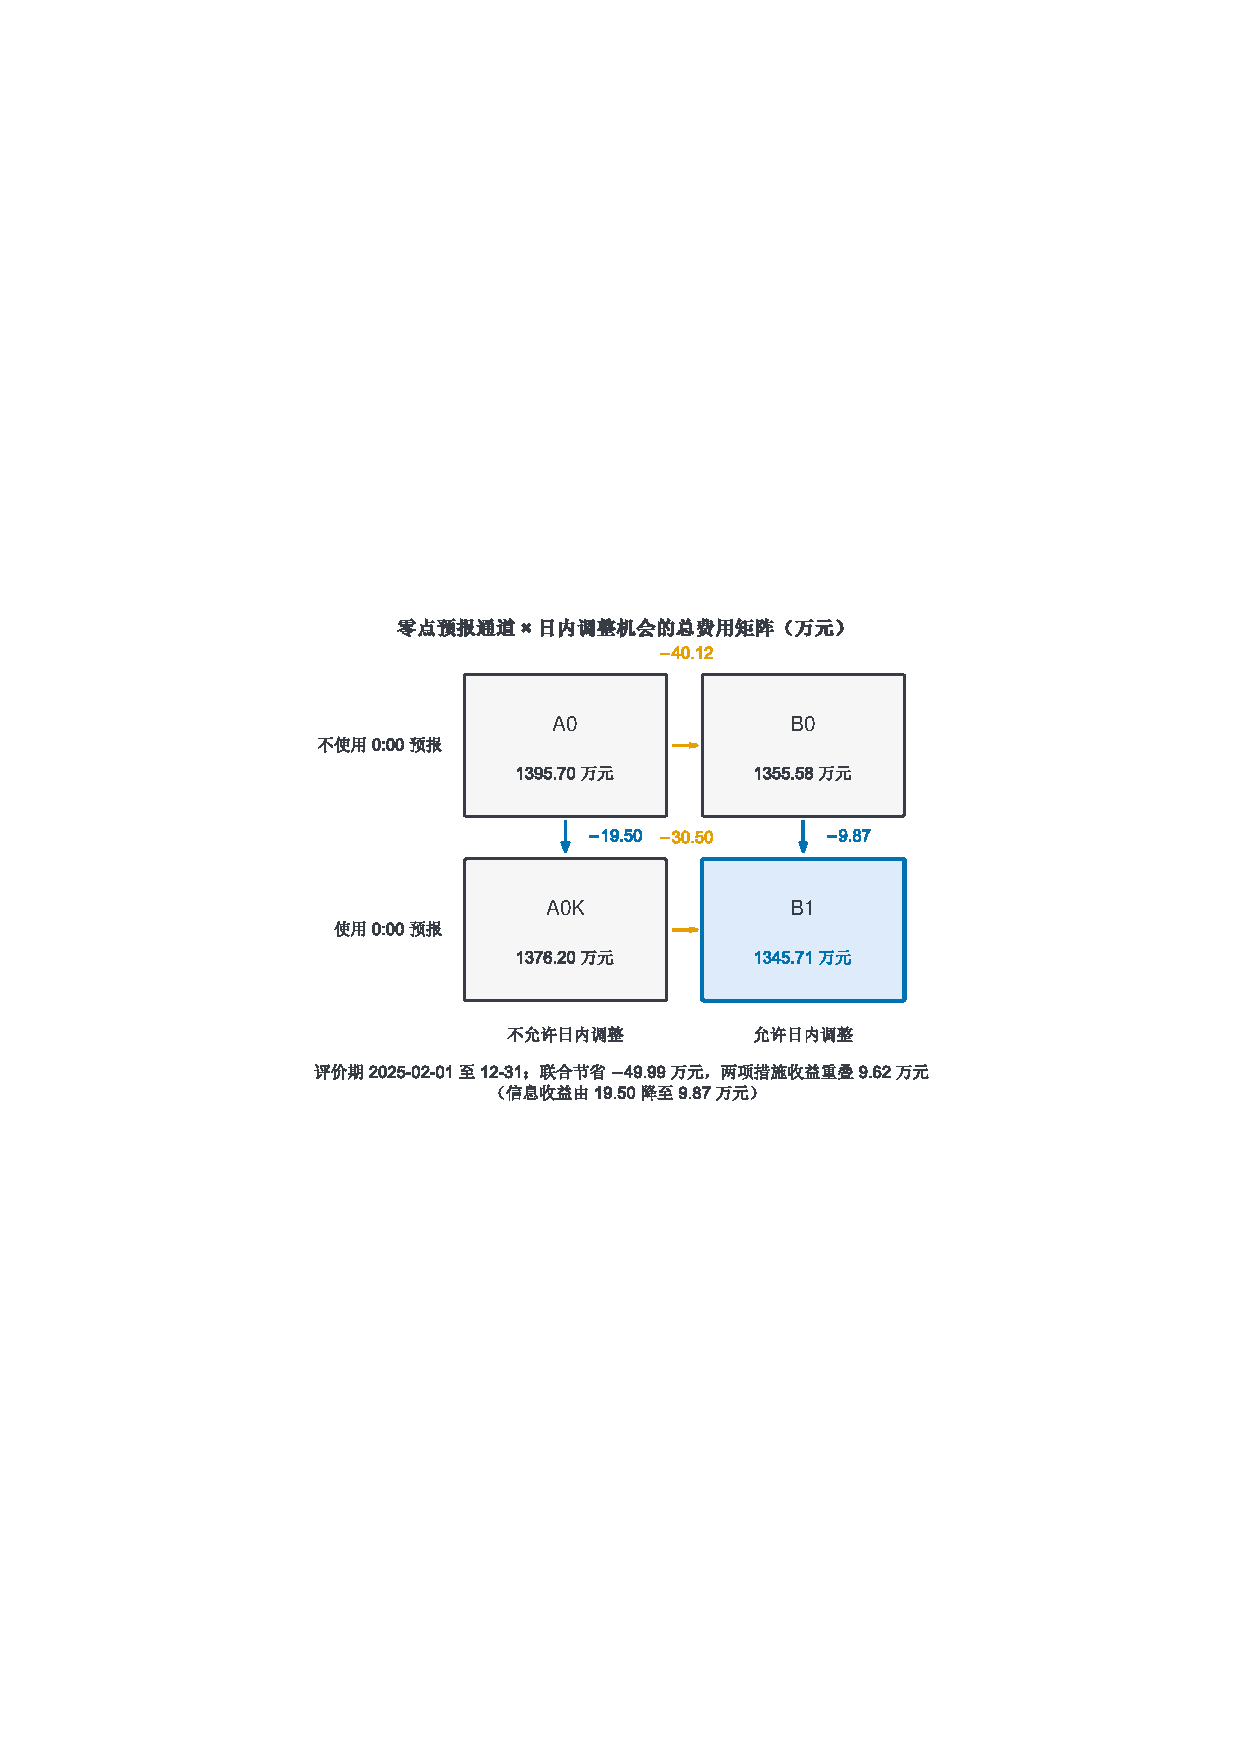
\includegraphics[width=0.8\textwidth]{p3_fig1.pdf}
  \caption{0:00 预报通道与日内调整机会的总费用矩阵（万元）}
  \label{fig:q3-matrix}
\end{figure}

由表~\ref{tab:q3-matrix} 与图~\ref{fig:q3-matrix} 可得三点结论：

\begin{enumerate}
  \item \textbf{A0 与问题二主方案完全重合}（1395.70 万元），说明问题二、问题三两条链路在同一评价口径下自洽——问题三的``不用预报通道、不允许调整''退化为问题二模型；
  \item 单独引入日内调整降费 \textbf{40.12 万元}，单独引入 0:00 预报通道降费 \textbf{19.50 万元}；在本文的数据上，\textbf{调整机会的价值约为预报通道的两倍}；
  \item 两项单独收益之和为 59.62 万元，而联合收益为 \textbf{49.99 万元}，\textbf{重叠 9.62 万元}。这说明两类改进\textbf{部分替代}：手中已有第二次决策机会时，0:00 预报的边际价值下降。因此两个数字不能简单相加，这正是必须做 $2\times2$ 对照而非单项消融的原因。
\end{enumerate}

B1 即本文问题三主方案，全年费用 \textbf{1345.71 万元}，相对问题二主方案节省 49.99 万元（$-3.58\%$）。

\subsection{指定日期的表 1、表 2、表 3 结果}
\label{sec:q3-tables}

按题目表 1、表 2、表 3 的格式，表~\ref{tab:q3-t1}--表~\ref{tab:q3-t3} 给出四个指定日期（2025 年 3 月 20 日、6 月 21 日、9 月 23 日、12 月 21 日）的完整结果，主方案为 B1。四个日期分别对应春分、夏至、秋分、冬至，覆盖评价期内负载与光伏的季节差异。

\textbf{表 1：指定时间段购电量。}表~\ref{tab:q3-t1} 给出题目指定的六个 10 分钟时段（10:00、12:00、14:00、16:00、18:00、20:00 起点）的购电量，以及全天计划购电量、调整后购电量与全日购电费（含调整附加费与紧急购电费）。可以看到：\textbf{六个指定时段的调整后购电量与 0:00 计划一致}——调整主要发生在非指定时段，故指定时段两列数值相同；全天口径下两者出现差异（例如 12 月 21 日为计划 98349.89 kWh、调整后 96906.82 kWh）。夏季（6 月 21 日）调整后全天购电量略高于计划（36911.13 对 36864.37 kWh）：该日光伏充沛、缺口少，调整的作用是把购电在时段间微调，上调部分按 1.5 倍计价，故购电量略增而附加费仅 29.28 元。

\begin{table}[htbp]
  \centering
  \caption{四个指定日期的购电量：六个指定时段（计划值与调整后值一致）与全天口径（kWh），以及全日购电费（元）}
  \label{tab:q3-t1}
  \footnotesize
  \setlength{\tabcolsep}{3.6pt}
  \begin{tabular}{lcccccccccc}
    \toprule
    日期 & 10:00 & 12:00 & 14:00 & 16:00 & 18:00 & 20:00
         & 全天计划 & 全天调整后 & 全日购电费 \\
    \midrule
    2025-03-20 & 0.00 & 554.52 & 0.00 & 567.05 & 701.86 & 0.00
               & 68944.02 & 68455.43 & 42081.89 \\
    2025-06-21 & 0.00 & 0.00 & 0.00 & 212.16 & 0.00 & 0.00
               & 36864.37 & 36911.13 & 20752.42 \\
    2025-09-23 & 0.00 & 411.45 & 0.00 & 512.77 & 770.17 & 0.00
               & 67064.04 & 66896.01 & 45106.35 \\
    2025-12-21 & 0.00 & 1039.77 & 0.00 & 845.05 & 735.21 & 0.00
               & 98349.89 & 96906.82 & 62694.46 \\
    \bottomrule
  \end{tabular}
\end{table}

计入紧急购电后，四日的合计购电量依次为 68525.56、36911.13、67365.51、96906.82 kWh；其中 3 月 20 日与 9 月 23 日发生紧急购电（表~\ref{tab:q3-t3}），6 月 21 日与 12 月 21 日为零。费用构成的差异同样清晰：3 月 20 日合同费 41441.26 元、调整附加费 151.45 元、紧急购电费 489.19 元；9 月 23 日紧急购电费升至 2825.21 元（晚峰缺口最重）；12 月 21 日合同费 62202.88 元，为四日最高，反映冬季高负载。

\textbf{表 2：指定时间段充放电量与 0:00、24:00 储电量。}表~\ref{tab:q3-t2} 给出六个 4 小时区间的充电量与放电量，以及 0:00、24:00 的储电量。四日都呈``凌晨与午间充电、早晚峰放电、深夜回充''的形态；储电量在日间两次触及上限附近、晚峰后回落，0:00 与 24:00 的差异反映实际储电量的跨日连续衔接（如 9 月 23 日 10585.62 $\to$ 10454.35 kWh，与 \S\ref{sec:q2-days} 中问题二同日的实测轨迹一致，说明该日的合同调整未改变执行层的物理动作）。

\begin{table}[htbp]
  \centering
  \caption{四个指定日期的六段 4 小时充放电量（kWh）与 0:00、24:00 储电量（kWh）}
  \label{tab:q3-t2}
  \footnotesize
  \setlength{\tabcolsep}{3.4pt}
  \begin{tabular}{llcccccccc}
    \toprule
    日期 & 项 & 0:00--4:00 & 4:00--8:00 & 8:00--12:00 & 12:00--16:00
         & 16:00--20:00 & 20:00--24:00 & 0:00 & 24:00 \\
    \midrule
    \multirow{2}{*}{03-20} & 充 & 133.27 & 325.08 & 6061.85 & 4210.58 & 46.14 & 10717.51 & \multirow{2}{*}{10800.00} & \multirow{2}{*}{10784.00} \\
                           & 放 & 189.75 & 5470.08 & 2777.38 & 268.95 & 5803.05 & 2915.68 & & \\
    \midrule
    \multirow{2}{*}{06-21} & 充 & 169.79 & 454.45 & 9377.58 & 0.00 & 105.32 & 10048.72 & \multirow{2}{*}{10800.00} & \multirow{2}{*}{10800.00} \\
                           & 放 & 3264.87 & 4836.61 & 0.00 & 0.00 & 5738.88 & 2485.90 & & \\
    \midrule
    \multirow{2}{*}{09-23} & 充 & 330.48 & 418.77 & 5595.42 & 4850.22 & 40.07 & 10298.83 & \multirow{2}{*}{10585.62} & \multirow{2}{*}{10454.35} \\
                           & 放 & 288.54 & 6361.61 & 1896.62 & 517.88 & 6099.83 & 2396.04 & & \\
    \midrule
    \multirow{2}{*}{12-21} & 充 & 94.48 & 974.65 & 6193.26 & 6327.44 & 9.61 & 10561.20 & \multirow{2}{*}{10800.00} & \multirow{2}{*}{10800.00} \\
                           & 放 & 172.00 & 1515.29 & 6891.61 & 2428.86 & 5719.83 & 2842.53 & & \\
    \bottomrule
  \end{tabular}
\end{table}

\textbf{表 3：紧急购电结果。}表~\ref{tab:q3-t3} 按题目表 3 格式给出紧急购电的购电时间段与购电量（连续区间已合并）。四日中仅 3 月 20 日与 9 月 23 日发生紧急购电，且全部集中在晚峰时段（20:20--21:50）：此时光伏退出、净负载抬升，若合同上调幅度不足或储能已接近下限，缺口便只能按 5 倍电价补足。9 月 23 日的三个事件（共 469.50 kWh）是四日中紧急购电最重的时段。

\begin{table}[htbp]
  \centering
  \caption{四个指定日期的紧急购电结果（合并连续区间）}
  \label{tab:q3-t3}
  \small
  \begin{tabular}{llcc}
    \toprule
    日期 & 购电时间段 & 购电量/kWh & 当日合计/kWh \\
    \midrule
    2025-03-20 & 20:30--20:40 & 70.12 & 70.12 \\
    \midrule
    2025-06-21 & 无 & 0 & 0 \\
    \midrule
    \multirow{3}{*}{2025-09-23} & 20:20--20:40 & 278.48 & \multirow{3}{*}{469.50} \\
                                & 20:50--21:10 & 129.61 & \\
                                & 21:20--21:50 & 61.40 & \\
    \midrule
    2025-12-21 & 无 & 0 & 0 \\
    \bottomrule
  \end{tabular}
\end{table}

上述四个日期的结果与全年 334 天的汇总口径一致；全部逐区间策略已按题目要求写入 \texttt{result3.xlsx}（含``计划购电量''``调整购电量''``充放电量''``紧急购电量''四张表）。

\subsection{主方案的日内形态与逐月费用}
\label{sec:q3-day}

\begin{figure}[htbp]
  \centering
  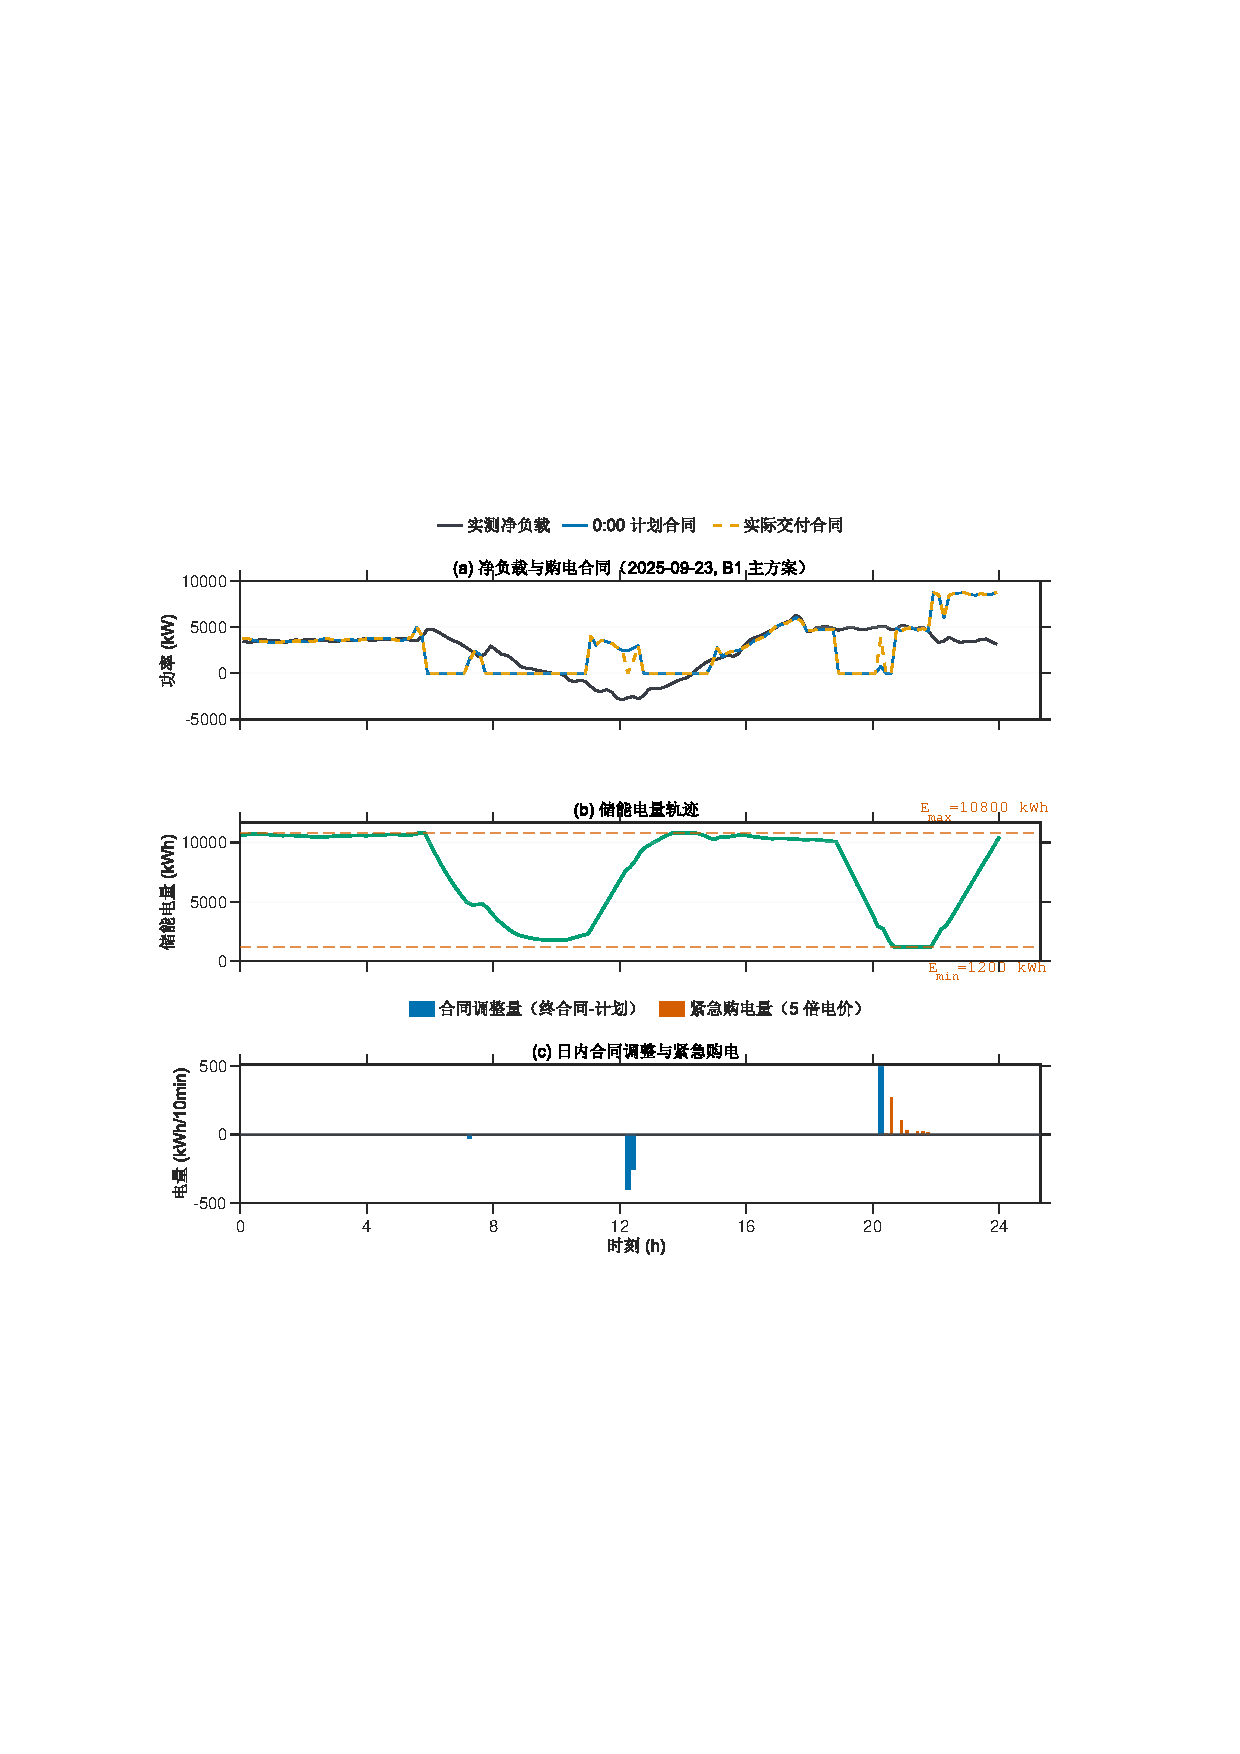
\includegraphics[width=0.86\textwidth]{p3_fig3.pdf}
  \caption{2025-09-23 主方案 B1 的日内调度：(a)~实测净负载、0:00 计划合同与实际交付合同；(b)~储能电量轨迹；(c)~日内合同调整量与紧急购电量}
  \label{fig:q3-day}
\end{figure}

以 2025-09-23 为例（图~\ref{fig:q3-day}）：0:00 计划的合同 $b^{\mathrm{plan}}$（图中浅色实线）与实际交付合同 $b$（虚线）在夜间与清晨几乎重合，主要调整发生在 12:00 时刻——该次求解把午后部分区间的合同\textbf{下调}（图~\ref{fig:q3-day}c 中 12 时附近的负向柱），下调部分只需按 $0.5p$ 支付违约费；20:00 前后晚峰光伏退出、净负载抬升，合同被\textbf{上调}并伴生紧急购电（图中橙色柱）。储能轨迹仍保持``白天光伏充沛时充电、晚峰放电''的日循环，日末储电量与日初衔接，与问题二同期的运行形态一致。

\subsection{其他时刻预报的引入必要性}
\label{sec:q3-other}

这是题面明确要求回答的问题。本节考察两种``把 6:00/12:00/18:00 预报真正用起来''的做法：

\begin{itemize}
  \item \textbf{全融合（B3）}：每个调整时刻 $\tau$ 都用当期附件 3 预报重估剩余时段的净负载，即把式~\eqref{eq:q3-fuse} 从``仅 0:00 通道''推广到``当期通道''；
  \item \textbf{门控（G）}：承认``用不用''本身是一个决策，在每个决策点用纯因果的历史回放，从融合强度 $\lambda\in\{0,\tfrac14,\tfrac12,1\}$ 中择一（$\lambda=0$ 即退回 B1）。
\end{itemize}

\subsubsection{预报精度的改善}

\begin{figure}[htbp]
  \centering
  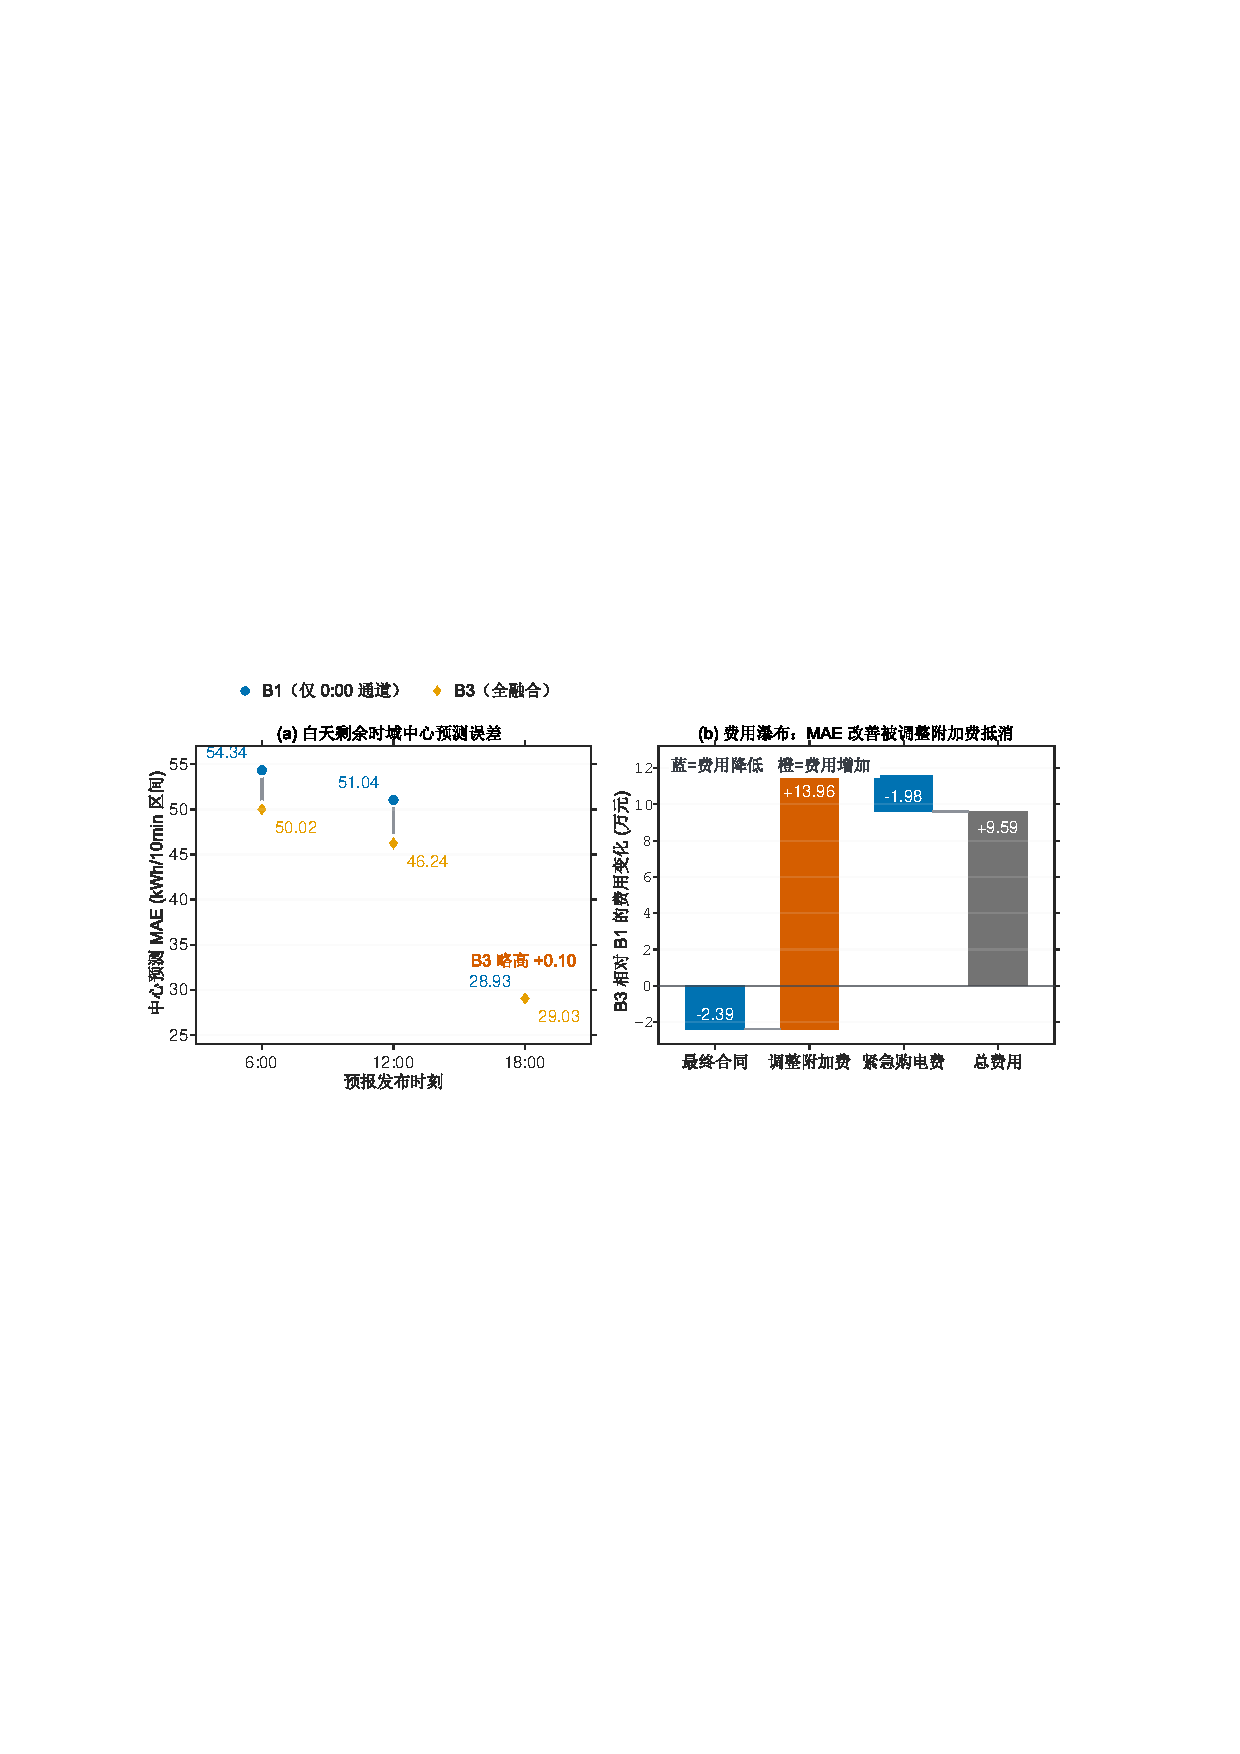
\includegraphics[width=0.95\textwidth]{p3_fig2.pdf}
  \caption{(a)~白天剩余时域中心预测 MAE（kWh/10\,min 区间）；(b)~全融合 B3 相对 B1 的费用瀑布}
  \label{fig:q3-mae}
\end{figure}

图~\ref{fig:q3-mae}a 给出白天剩余时域的中心预测平均绝对误差：全融合 B3 在 6:00 与 12:00 两个发布时刻将 MAE 由 54.34、51.04 降至 50.02、46.24，降幅分别为 4.32 与 4.80；18:00 时刻略升 0.10（28.93 $\to$ 29.03），原因是该时刻距当日光伏结束已近，可改进的时域很短。

\begin{figure}[htbp]
  \centering
  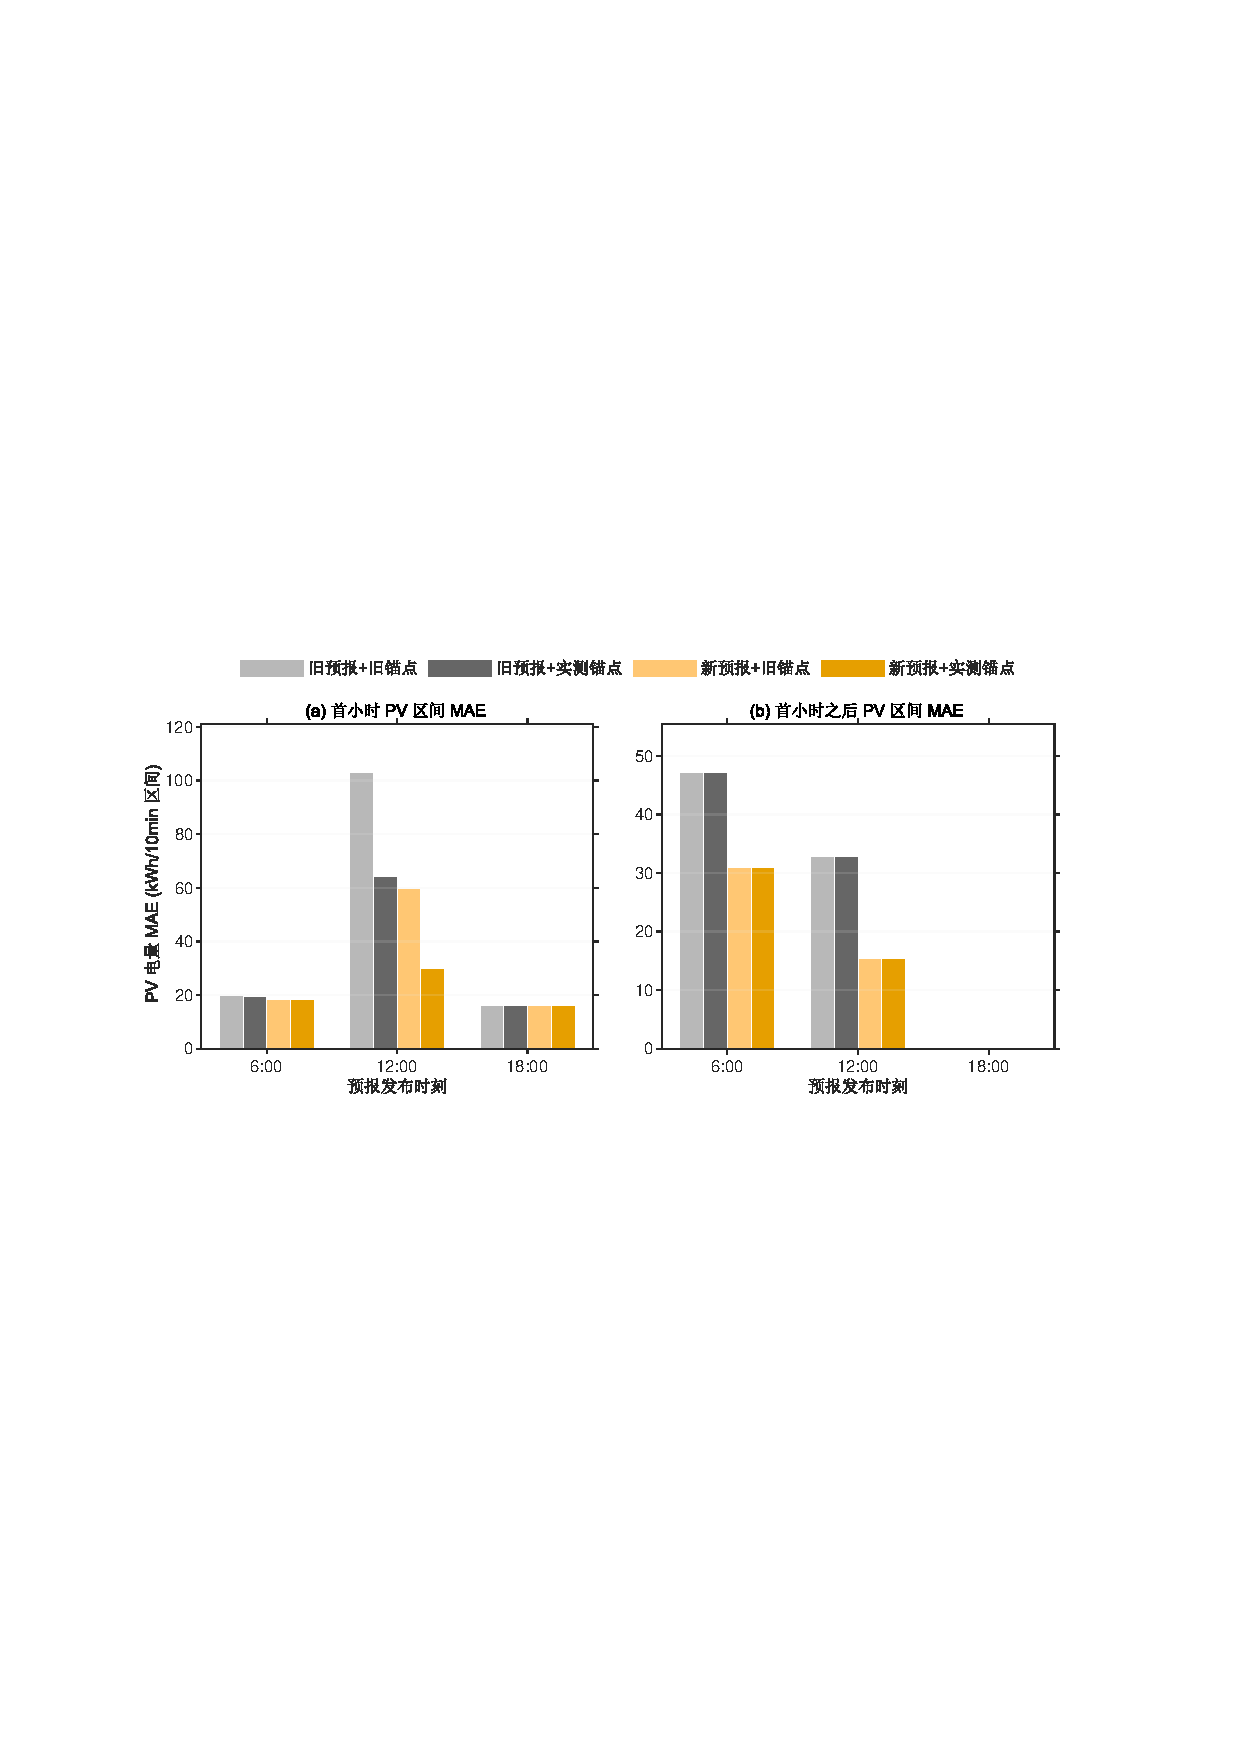
\includegraphics[width=0.95\textwidth]{p3_fig5.pdf}
  \caption{光伏区间电量 MAE：预报来源（历史预报／附件 3 预报）与端点锚定方式（历史锚点／实测锚点）的四种组合，(a)~发布后首小时；(b)~首小时之后}
  \label{fig:q3-pv}
\end{figure}

图~\ref{fig:q3-pv} 进一步在光伏区间电量本身上作四项对照。附件 3 预报叠加实测锚点的组合在两个时段上整体误差最低，且改进集中在\textbf{发布后首小时}（图~\ref{fig:q3-pv}a）——12:00 时刻的四种组合差异最大，说明当日上午实测量已经足以校正当日的光伏形状。这为式~\eqref{eq:q3-pv} 中用实测水平锚定端点的做法提供了直接依据。

\subsubsection{总费用的上升}

图~\ref{fig:q3-mae}b 给出 B3 相对 B1 的费用瀑布（表~\ref{tab:q3-b3}）：最终合同费用与紧急购电费用均略有下降，但\textbf{调整附加费大幅上升}，合计总费用上升。

\begin{table}[H]
  \centering
  \caption{全融合 B3 相对主方案 B1 的费用变化（评价期 334 天，万元）}
  \label{tab:q3-b3}
  \begin{tabular}{lcc}
    \toprule
    费用项 & 变化量 & 方向 \\
    \midrule
    最终合同费用 & $-2.39$ & 略降（更准的预测选中了更便宜的合同） \\
    调整附加费 & $+13.96$ & \textbf{显著上升（主导项）} \\
    紧急购电费 & $-1.98$ & 略降 \\
    \midrule
    合计 & $+9.59$ & \textbf{总费用上升} \\
    \bottomrule
  \end{tabular}
\end{table}

机制是明确的：精度更高的点预测使线性规划\textbf{更倾向于}偏离 0:00 计划而转向低价时段，而每一次偏离都需按 $0.5p$／$1.5p$ 付费；附加费的增量（13.96 万元）远大于合同费用与紧急费用节省之和（4.37 万元）。即\textbf{双向违约价将``精度更高的日前预测''转化为``更频繁的合同偏离''}。

\subsubsection{逐决策点自适应门控的结果}

\begin{figure}[htbp]
  \centering
  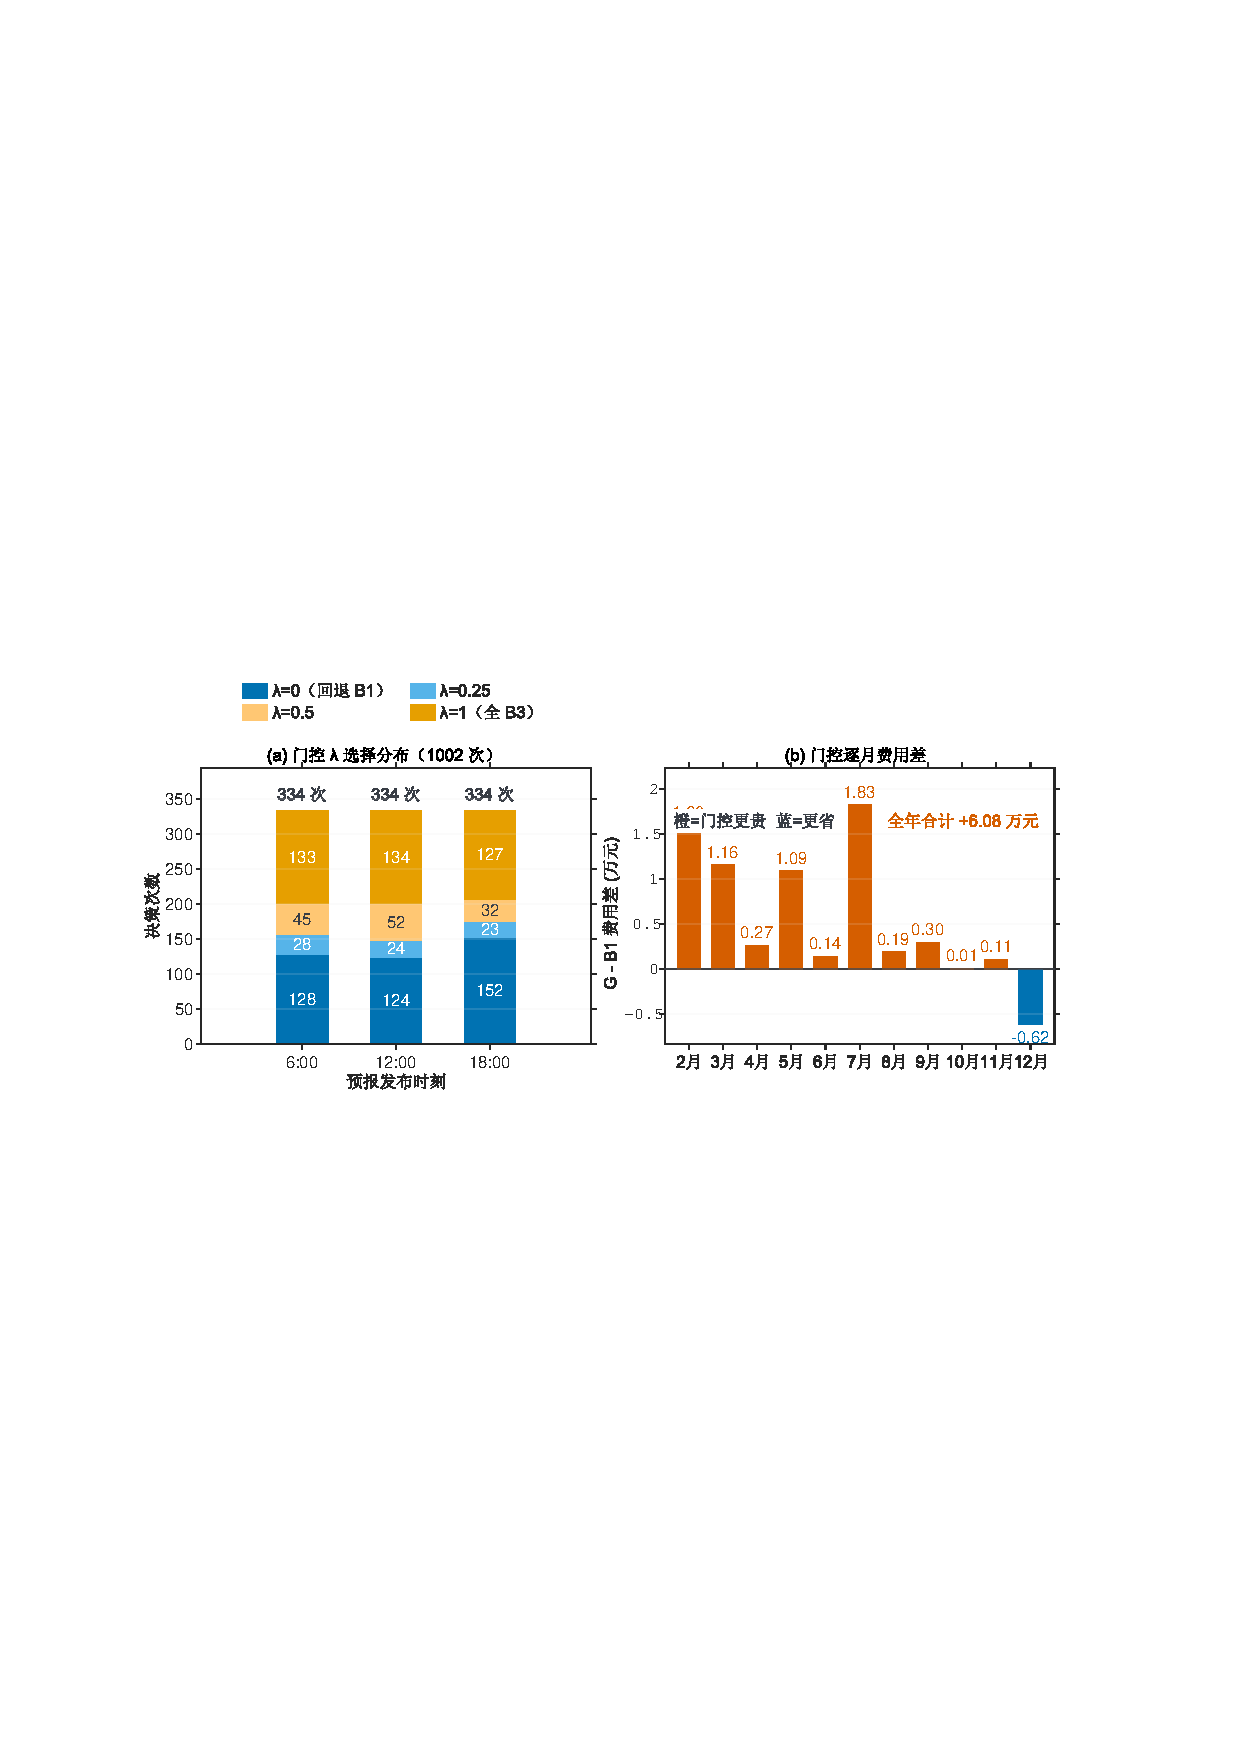
\includegraphics[width=0.96\textwidth]{p3_fig6.pdf}
  \caption{(a)~门控 $\lambda$ 在 1002 个决策点上的选择分布；(b)~门控方案 G 相对 B1 的逐月费用差（橙色表示门控方案费用更高，蓝色表示更低）}
  \label{fig:q3-gate}
\end{figure}

图~\ref{fig:q3-gate}a 给出门控 G 在全部 1002 个决策点（334 天 $\times$ 3 个调整时刻）上的选择分布：6:00 时刻 $\lambda=0$ 与 $\lambda=1$ 分别为 128 与 133 次，12:00 时刻为 124 与 134 次，18:00 时刻为 152 与 127 次，两个端点档位合计均占约七至八成，中间档位（$\lambda=0.25,0.5$）合计不足三成。这本身即表明：\textbf{在单一决策点层面难以判断融合是否有利}，预测精度与结算费用之间的方向并不总是一致，因此门控退化为在两个端点之间选择。

其结果是门控方案全年比 B1 高 \textbf{6.08 万元}（图~\ref{fig:q3-gate}b）：11 个月中仅 12 月为负（$-0.62$ 万元），2 月与 7 月增量最大（分别为 1.60 与 1.83 万元）。

\begin{figure}[htbp]
  \centering
  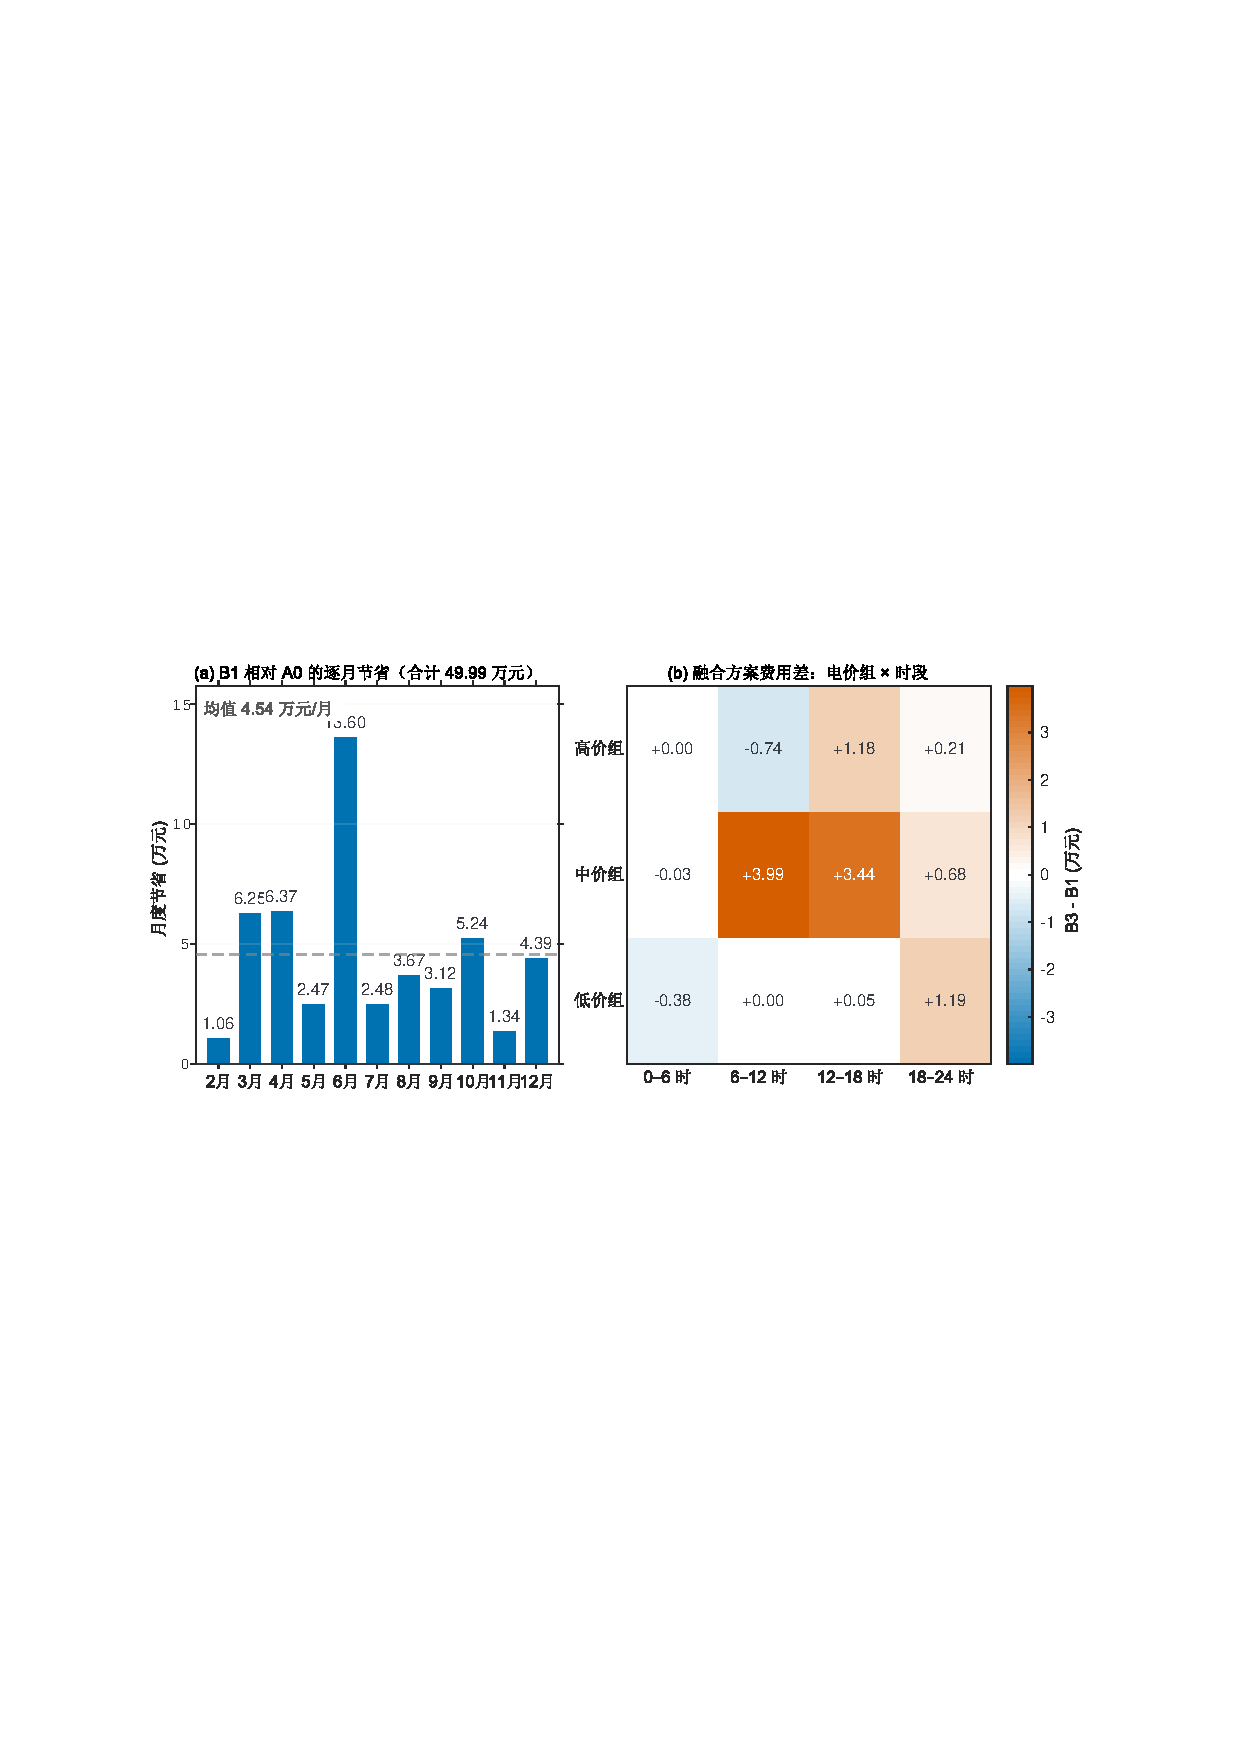
\includegraphics[width=0.96\textwidth]{p3_fig4.pdf}
  \caption{(a)~B1 相对 A0 的逐月节省（合计 49.99 万元，均值 4.54 万元/月）；(b)~全融合方案费用差的分组热力图（B3 $-$ B1）}
  \label{fig:q3-month}
\end{figure}

图~\ref{fig:q3-month}a 给出主方案 B1 相对基准 A0 的逐月节省：11 个月\textbf{全部为正}，合计 49.99 万元、均值 4.54 万元/月，其中 6 月最高（13.60 万元），与 \S\ref{sec:q2-year} 中 6 月紧急费用最集中相呼应——夏季晚峰缺口最需要日内的第二次决策。图~\ref{fig:q3-month}b 进一步按``电价组 $\times$ 时段''分解 B3 与 B1 的费用差：正值集中在 6--18 时的\textbf{中价组}（$+3.99$、$+3.44$），正是合同最可能被反复调整、违约附加费最易触发的时段；低价组与高价组多数取值接近零或为负，说明融合的代价并非均匀分布，而是集中在中间价位区间。

\subsubsection{小结}

在本文的结算口径与所考察的网格范围内，\textbf{不需要引入其他时刻的预报来制定调整购电策略}。附件 3 的信息\textbf{在 0:00 通道使用一次}（方案 B1，1345.71 万元）即已足够；6:00、12:00、18:00 的预报只需用于``按实测重新校正剩余时段合同''这一项工作，不必再作为新的预测输入反复重建预测。其原因不在于预报精度——附件 3 的逐时预报精度更高（图~\ref{fig:q3-mae}a、图~\ref{fig:q3-pv}）——而在于本题的双向违约价显著削弱了``预测更准''向``费用更低''的转化渠道：预测精度提高带来的合同费用与紧急费用节省（4.37 万元）不足以补偿由此增加的违约附加费（13.96 万元）。

\textbf{适用范围说明。}该结论是在``偏差对 0:00 计划计量、附加费 $0.5p$/$1.5p$、紧急价 $5p$''这套结算口径下，以及本文所考察的全融合与门控两种形式下成立的。若结算口径改变（例如允许无成本无限次调整，或偏差改为对上一次合同计量），结论需要重新核验；本文不据此断言``其他时刻预报无信息价值''。

% =========================================================================
% 八、问题四（留白待补）
% =========================================================================

\section{问题四：波动电价下的模型建立与求解（待补充）}

% 题面要点备忘：
% 1. 外网电价实时波动（附件 4 提供 2025 年逐日逐时段电价）；
% 2. 针对波动电价建立微网当天购电策略的数学模型；
% 3. 在波动电价下重新计算问题 2 与问题 3；
% 4. 结果分别保存至 result4-2.xlsx（对应问题 2）与 result4-3.xlsx（对应问题 3）。
（本部分留白，待后续补充。）

% =========================================================================
% 九、模型评价
% =========================================================================

\section{模型评价与改进（问题一至问题四）}

本节只陈述有证据支持的具体性质。评价分两层：先说清``好在哪、由什么证据支持、在什么范围内成立''，再说``局限对应哪一项实质性改进''。

\subsection{模型的具体优势及其证据}

\begin{enumerate}
  \item \textbf{子问题可求全局最优且计算量小。}问题一至问题四的计划层与调整层都是线性规划，规模为百至千量级变量，用 HiGHS 求解在秒级完成；问题一的充放电互斥约束经命题保证线性松弛在最优值意义下精确（\S\ref{sec:q1-relax}），问题三的含分段结算规则也被化归为\emph{单个}线性规划（式~\eqref{eq:q3-adjust}），无需二元变量。相应地，{\bfseries 主方案给出的最优性是针对给定输入、给定约束的确定性子问题的最优性}，不是对整条滚动策略的整体最优性。
  \item \textbf{执行规则完全因果、可行域明确。}式~\eqref{eq:q2-exec} 的尽限充放电规则只依赖当前区间的实测净负载与当前实际库存，充放互斥由净缺口符号自动决定，实际库存始终落在 $[1200,10800]$ kWh 内；把实测净负载设为计划所用序列时，执行器逐位复现线性规划的解（\S\ref{sec:q2-exec}）。
  \item \textbf{实际库存跨日连续。}$E_H^{(d)}$ 直接结转成为 $E_0^{(d+1)}$，评价期 334 天内跨日衔接误差为 0，不存在人为重置库存带来的虚假收益。
  \item \textbf{账单可独立复算。}Q1 的购电费、Q2 的计划费与紧急费、Q4 两分支的合同费与附加费，均由不调用调度代码的独立路径重算并逐位吻合（\S\ref{sec:q1-constraint}、\S\ref{sec:q2-exec}、\S\ref{sec:q4-check}）。
  \item \textbf{$2\times2$ 对照能区分``信息''与``调整机会''。}问题三用``是否用 0:00 预报通道 $\times$ 是否允许日内调整''的四格设计，把两类改进的贡献与二者 9.62 万元的重叠分开计量（\S\ref{sec:q3-matrix}），避免了单项消融无法处理的相互替代问题。
  \item \textbf{预测器形式与参数取值受因果协议约束。}问题二的 $(\beta,W,\gamma,N_{\mathrm{DOW}})$ 按逐月 walk-forward 选取，问题三的 $\kappa_g$ 只用 $d$ 之前 30 天逐日重估，问题四的日内价格通道经``扰动未来电价、预测不变''的检验。问题三、问题四的固定配置为同年探索性选定，本文如实标注而不宣称独立测试（\S\ref{sec:q4-limit}）。
  \item \textbf{结论的边界被显式写出。}问题三``日内新增预报未进一步降低费用''限于所比较的全融合与门控两种策略、以及本文的结算口径（\S\ref{sec:q3-other}）；问题四的价格侧差额限于 24 小时固定策略（\S\ref{sec:q4-ablation}）；容量边际价值限于``固定下限、抬升上限''的扰动路径（\S\ref{sec:q1-sens}）。
\end{enumerate}

\subsection{局限与对应的实质性改进}

\begin{table}[htbp]
  \centering
  \caption{主要局限与对应的实质性改进方向}
  \label{tab:limits}
  \small
  \begin{tabularx}{\textwidth}{XX}
    \toprule
    当前的局限 & 对应的实质改进 \\
    \midrule
    预测精度指标（MAE）与实际结算费用方向不一致：问题三、问题四都出现``预测更准但费用未降'' & 在历史滚动验证中\textbf{直接用真实结算费用}为目标，去校准风险裕量水平与预报融合权重，而不是先优化 MAE 再检验费用 \\
    日前规划没有把未来的调整机会内生化：计划层按点预测求解，未考虑 6/12/18 时仍可重定合同 & 研究受非预见性约束的多阶段决策，或保持同一因果执行器、以回放费用重评各候选计划 \\
    48 小时时域的次日输入为``当日预测平铺''的持久性预测 & 加入只依赖当时历史的星期与季节条件预测，并在同一窗口下作对照 \\
    固定策略按同年结果探索性选择（问题三的 $\kappa_g$ 网格、问题四的 $(\lambda_{\mathrm{p}},\delta)$ 与时域） & 在后续独立年份上验证，或按本文方式如实保留``探索性、未做外部测试''的定位 \\
    未计电池退化、未建模售电与逆变器限制 & 在推广模型中加入循环成本、售电价与逆变器约束，并重新检验互斥松弛的精确性条件 \\
    风险裕量按各时段独立取分位数，未建模时段相关性 & 引入时段间相关结构（如情景集合或分层分位），并检验其对紧急费用的影响 \\
    \bottomrule
  \end{tabularx}
\end{table}

\subsection{关于创新点的表述}

本文的创新应表述为\textbf{针对本题所作的结构设计及其验证}，而不宣称算法本身原创：其一是把含双向违约价的调整决策化归为单个线性规划（式~\eqref{eq:q3-adjust}），使合同重定仍可求子问题最优；其二是用 $2\times2$ 对照分离``新增信息''与``调整机会''的贡献并量化二者重叠；其三是在波动电价下先厘清价格缩放不变性的适用边界，再以加权裕量与 48 小时时域分别处理价格结构与库存配置，并用同政策对照与放松下界界定各结论的范围。本文的主方案是线性规划与尽限反馈的组合，故不以动态规划的状态价值函数或深度学习方法作为全篇核心贡献；建模过程中测试过但未取得优势的做法（如逐情景回放择优的在线选择器）只作为负结果如实报告，不与主模型并列。


\clearpage
% =========================================================================
% 参考文献
% =========================================================================

% 参考文献单独存放在此文件。
% 在正文中使用 \cite{条目标签} 引用；每个 \bibitem 的标签应唯一。
% 每条文献都对应正文中确实使用的概念、公式或算法，不列入仅讨论过而未采用的方法。
\begin{thebibliography}{9}

  \bibitem{highs}
  Huangfu, Q., and Hall, J. A. J. Parallelizing the dual revised simplex method.
  \textit{Mathematical Programming Computation}, 10(1): 119--142, 2018.
  DOI: 10.1007/s12532-017-0130-5.

  \bibitem{scipy}
  Virtanen, P., Gommers, R., Oliphant, T. E., et al.
  SciPy 1.0: fundamental algorithms for scientific computing in Python.
  \textit{Nature Methods}, 17: 261--272, 2020.

  \bibitem{newsvendor}
  Arrow, K. J., Harris, T., and Marschak, J. Optimal inventory policy.
  \textit{Econometrica}, 19(3): 250--272, 1951.

  \bibitem{hyndman}
  Hyndman, R. J., and Athanasopoulos, G.
  \textit{Forecasting: Principles and Practice}, 3rd ed.
  OTexts, 2021. \S5.10 Time series cross-validation.
  \url{https://otexts.com/fpp3/tscv.html}

  \bibitem{mpc}
  Mayne, D. Q., Rawlings, J. B., Rao, C. V., and Scokaert, P. O. M.
  Constrained model predictive control: Stability and optimality.
  \textit{Automatica}, 36(6): 789--814, 2000.

\end{thebibliography}


\appendix
% =========================================================================
% 附录：支撑材料清单、软件环境、图表对应关系与核心程序
% =========================================================================

\section{支撑材料文件列表}

\subsection{输入数据（题面附件）}

\begin{itemize}
  \item \texttt{data/附件1.xlsx}：代表日逐 10 分钟的电价、小区负载与光伏预测功率（题面附件 1）；
  \item \texttt{data/附件2.xlsx}：2025 年逐日实测负载（工作表 1）与光伏功率（工作表 2）（题面附件 2）；
  \item \texttt{data/附件3.xlsx}：0:00、6:00、12:00、18:00 发布的未来 24 小时整点光伏功率预报（题面附件 3）；
  \item \texttt{data/附件4.xlsx}：2025 年逐日逐 10 分钟区间的实时电价（题面附件 4）；
  \item \texttt{data/附件5/}：官方提交模板（\texttt{result1.xlsx}、\texttt{result2.xlsx}、\texttt{result3.xlsx}、\texttt{result4-2.xlsx}、\texttt{result4-3.xlsx}），用于核对各工作簿的工作表名与原始行序。原始数据与模板均按题目要求随支撑材料提交，不在压缩包内重复打包。
\end{itemize}

\subsection{提交结果工作簿}

\begin{table}[H]
  \centering
  \caption{提交结果工作簿、工作表与生成入口}
  \label{tab:app-workbooks}
  \small
  \setlength{\tabcolsep}{4pt}
  \begin{tabularx}{\textwidth}{l>{\raggedright\arraybackslash}Xl}
    \toprule
    文件 & 工作表 & 生成入口 \\
    \midrule
    \texttt{results/result1.xlsx} & 计划购电量、充放电量 & \texttt{scripts/q1\_solve.py} \\
    \texttt{results/result2.xlsx} & 计划购电量、充放电量、紧急购电量 & \texttt{scripts/q2\_finalize\_E.py} \\
    \texttt{问题三/result3.xlsx} & 计划购电量、调整购电量、充放电量、紧急购电量 & \texttt{问题三/代码/} \\
    \texttt{问题四/result4-2.xlsx} & 计划购电量、充放电量、紧急购电量 & 问题四链路 \\
    \texttt{问题四/result4-3.xlsx} & 计划购电量、调整购电量、充放电量、紧急购电量 & 问题四链路 \\
    \bottomrule
  \end{tabularx}
\end{table}

五个工作簿的工作表名与官方模板逐一对应，其中前四个已按模板行序核对；问题三的 \texttt{result3.xlsx} 由问题三链路生成，未纳入本文的核验清单（见 \S\ref{app:audit}）。

\subsection{计算脚本}

以下脚本按问题分组；\textbf{每问只有一个复现入口}，其余脚本为该问的分析、配图或档案工具。

\begin{itemize}
  \sloppy \footnotesize
  \item \textbf{问题一}：主程序 \texttt{scripts/q1\_solve.py} 是本问的唯一入口，完成线性规划装配、求解、独立校验并写出 \texttt{result1.xlsx}；敏感性分析由 \texttt{scripts/q1\_analysis.py} 完成，涵盖无储能基准、容量与功率敏感性以及边际价值；配图由 \texttt{scripts/q1\_figures.py} 与 \texttt{scripts/q1\_analysis\_figures.py} 生成，前者绘制代表日输入与最优策略，后者绘制敏感性与边际价值曲线。
  \item \textbf{问题二入口}：主程序 \texttt{scripts/q2\_finalize\_E.py} 是本问的唯一入口，复现评价期总费用、生成三张指定日期结果表并写出 \texttt{result2.xlsx}。
  \item \textbf{问题二辅助}：选参由 \texttt{scripts/q2\_dow\_N\_joint.py} 完成，回放 36 个候选并给出逐月 walk-forward 日程；月度费用与风险档案由 \texttt{scripts/q2\_V\_dow\_N\_profile.py} 生成；\texttt{scripts/q2\_model.py} 回放早期的对照方案 A--D，\texttt{scripts/q2\_improve.py} 则用于预测器形式与执行规则的改进对照。
  \item \textbf{问题三}：\texttt{问题三/代码/} 下的模块实现附件 3 的预报通道、分档收缩回归、调整层线性规划与分段执行；\texttt{问题三/图片/} 存放该问的结果图。
  \item \textbf{问题四}：\texttt{问题四/代码/} 下的模块实现 48 小时滚动时域的计划与调整线性规划、尽限执行与全年回放；\texttt{scripts/q4\_export\_pt.py} 导出问题二预测器的中心预测序列，作为该问链路的输入。
  \item \textbf{图源文件}：\texttt{问题一/图片/fig*.fig} 与 \texttt{问题二/图片/fig*.fig} 为问题一、问题二配图的图源文件。
\end{itemize}

问题四的运行需先执行 \texttt{q4\_export\_pt.py} 生成需求代理序列，该依赖为单向前置关系；除此之外，四问的复现入口互不重叠，不存在同一问被两个脚本各自声称唯一入口的情况。

\subsection{中间结果}

\begin{itemize}
  \sloppy \small
  \item 问题一：\texttt{results/q1\_summary.json}（解与校验）、\texttt{results/q1\_analysis.json}（敏感性与边际价值）、\texttt{results/q1\_solution.npz}（求解器输出）。
  \item 问题二：\texttt{results/q2\_dow\_N\_joint.json}（选参日程）、\texttt{results/q2\_V\_dow\_N\_profile.json}（月度与风险档案）、\texttt{results/q2\_E\_tables.json}（指定日期表格）。
  \item 问题四的输入之一：\texttt{results/q4\_v3/F\_pt.csv}，即问题二预测器的中心预测序列（$365\times144$）。
\end{itemize}

上述中间结果均由其对应脚本自动生成，不含手工编辑的数值。除 \texttt{F\_pt.csv} 是问题四链路的必要输入外，其余中间结果不参与任何论文数值的最终生成：论文中的数字一律由脚本在运行时直接输出。

\section{软件环境与依赖版本}

\begin{table}[H]
  \centering
  \caption{运行环境与依赖版本（实际使用版本）}
  \label{tab:app-env}
  \small
  \begin{tabularx}{\textwidth}{l>{\raggedright\arraybackslash}X}
    \toprule
    组件 & 版本／说明 \\
    \midrule
    Python & 3.13.14 \\
    NumPy & 2.5.2 \\
    SciPy & 1.18.1（线性规划经 \texttt{scipy.optimize.linprog} 调用 HiGHS 求解器） \\
    pandas & 3.0.5（读取 \texttt{.xlsx} 输入） \\
    openpyxl & 3.1.5（写出提交工作簿） \\
    MATLAB & 用于问题一、问题二配图的图源文件（\texttt{.fig}），不作为求解器使用 \\
    \bottomrule
  \end{tabularx}
\end{table}

全部脚本以项目根目录为基准解析相对路径（即以脚本文件所在目录的两级父目录为根），源码中不含任何个人绝对路径，可在任意目录放置后直接运行。

\section{论文图表与数据、脚本的对应关系}

\begin{table}[H]
  \centering
  \caption{论文主要图表与配置、数据文件、生成脚本的对应关系}
  \label{tab:app-map}
  \footnotesize
  \setlength{\tabcolsep}{4pt}
  \begin{tabularx}{\textwidth}{l>{\raggedright\arraybackslash}Xl}
    \toprule
    论文图表 & 对应配置与数据 & 生成脚本 \\
    \midrule
    表~\ref{tab:q1-t1}、表~\ref{tab:q1-t2} & 问题一最优解；\texttt{data/附件1.xlsx} & \texttt{q1\_solve.py} \\
    表~\ref{tab:q1-compare} & 无储能基准与主方案 & \texttt{q1\_analysis.py} \\
    图~\ref{fig:q1-input}--图~\ref{fig:q1-sens}（问题一） & 代表日输入、最优策略、敏感性与边际价值 & \texttt{q1\_figures.py}、\texttt{q1\_analysis\_figures.py} \\
    表~\ref{tab:q2-sched} & 36 候选逐月 walk-forward & \texttt{q2\_dow\_N\_joint.py} \\
    表~\ref{tab:q2-total}、表~\ref{tab:q2-t1}--表~\ref{tab:q2-t3} & 主方案 E；\texttt{data/附件1,2.xlsx} & \texttt{q2\_finalize\_E.py} \\
    表~\ref{tab:q2-month}、表~\ref{tab:q2-risk} & 主方案月度与风险档案 & \texttt{q2\_V\_dow\_N\_profile.py} \\
    表~\ref{tab:q2-ladder}、图~\ref{fig:q2-ladder} & 对照方案 A--E 的水平比较 & \texttt{q2\_model.py}（回放）、\texttt{q\_paper\_figures.py}（绘图） \\
    图~\ref{fig:q2-frame}--图~\ref{fig:q2-emerg}（问题二） & 主方案 E 的框架、预测、指定日、全年与风险 & \texttt{问题二/图片/fig*.fig} 导出 \\
    表~\ref{tab:q3-matrix}、表~\ref{tab:q3-b3} & 问题三 $2\times2$ 矩阵与 B3 费用分解 & \texttt{问题三/代码/} \\
    图~\ref{fig:q3-matrix}--图~\ref{fig:q3-month}（问题三） & 矩阵、MAE 与费用瀑布、日内形态、门控与逐月 & \texttt{问题三/图片/fig*.pdf} \\
    表~\ref{tab:q4-struct}、图~\ref{fig:q4-struct} & 附件 4 价格结构（可直接复算） & 复算脚本 \\
    表~\ref{tab:q4-main}、表~\ref{tab:q4-horizon} & 主方案 F\_48／G\_48 与时域对照 & 问题四链路 \\
    图~\ref{fig:q4-horizon}、图~\ref{fig:q4-ladder}、图~\ref{fig:q4-regret} & 时域机制、方案阶梯、参照对比 & \texttt{问题四/照片/fig*.pdf} \\
    \bottomrule
  \end{tabularx}
\end{table}

\section{校验与审计的分项说明}
\label{app:audit}

\begin{table}[H]
  \centering
  \caption{审计分项、覆盖范围与结果}
  \label{tab:app-audit}
  \footnotesize
  \setlength{\tabcolsep}{4pt}
  \begin{tabularx}{\textwidth}{l>{\raggedright\arraybackslash}Xl}
    \toprule
    审计项 & 覆盖范围 & 结果 \\
    \midrule
    物理守恒（区间能量平衡） & 问题一单日；问题二评价期 334 天；问题四全部 20 条轨迹 & 最大残差 $\le1.2\times10^{-13}$ kWh（Q2）、$<10^{-7}$（Q4） \\
    储能电量边界 & 同上 & 全程位于 $[1200,10800]$ kWh \\
    充放电功率上限 & 同上 & 无越界；同时充放电重叠量为 0 \\
    费用账本 & 问题一全天费用；问题二计划费与紧急费；问题四两分支合同费与附加费 & 与独立复算路径逐位吻合 \\
    时间映射 & \texttt{result1.xlsx}、\texttt{result2.xlsx} 与字面时钟区间 & 模板行标签整体后移一个区间，两口径相差 10 分钟 \\
    结果模板 & 四个已生成工作簿的工作表名与行序 & 与官方模板一致；\texttt{result3} 未纳入本次核验 \\
    可复现性 & 问题一、问题二主链路 & 可由原始附件直接复现；问题四需先运行 \texttt{q4\_export\_pt.py} \\
    \bottomrule
  \end{tabularx}
\end{table}

需要区分``一致''与``正确''：``沿用旧脚本得到逐位相同的数值''只能证明两次运行一致，不能证明旧口径本身正确。因此上表中凡涉及账本与模板的项，均由\emph{不调用调度代码}的独立路径重算，而不是与原脚本自比。

\section{核心程序}

本节给出问题一、问题二与问题四核心模块的\textbf{完整源码}（三个文件即对应链路的核心实现，可独立阅读），其余辅助模块（问题一敏感性分析、问题二选参与风险档案、问题三预报融合与调整层、问题四全量回放与核验）见上文 \S 的脚本清单，随支撑材料按目录结构提交。

\subsection{问题一：线性规划装配、求解与独立复核}
\label{app:q1-code}

\VerbatimInput[frame=single,numbers=left,fontsize=\scriptsize,label=\texttt{code/q1\_core.py}]{code/q1_core.py}

\subsection{问题二：预测—计划—执行三层框架核心代码}
\label{app:q2-code}

\VerbatimInput[frame=single,numbers=left,fontsize=\scriptsize,label=\texttt{code/q2\_core.py}]{code/q2_core.py}

\subsection{问题四：48 小时滚动时域计划、调整与执行核心代码}
\label{app:q4-code}

\VerbatimInput[frame=single,numbers=left,fontsize=\scriptsize,label=\texttt{code/q4\_core.py}]{code/q4_core.py}


\end{document}
